\documentclass[11pt]{report}

\usepackage[utf8]{inputenc}
\usepackage[T1]{fontenc}
\usepackage{lmodern}
\usepackage[english]{babel}
\usepackage[a4paper,width=150mm,top=25mm,bottom=25mm,marginparwidth=80pt]{geometry}

\usepackage[style=numeric,backend=biber,sorting=none]{biblatex}
% run 'biber --output_format=bibtex --output_resolve main.bcf' to remove duplicates and unused, format and sort
\addbibresource{main_biber.bib}

\usepackage{amsmath}
\usepackage{siunitx}
\sisetup{
  round-mode      = places, % rounds numbers
  round-precision = 2,      % to 2 places
}

% To prevent floats from floating too much...
\usepackage{float}
\usepackage{placeins}

% For tables formatting
\usepackage{array, booktabs, caption, makecell, multirow}
\renewcommand\theadfont{\bfseries}

\usepackage{graphicx}
\graphicspath{ {images/}}

\setlength{\headheight}{14pt}
\usepackage{fancyhdr}
\pagestyle{fancy}
\fancyhead{}
% \fancyhead[RO,LE]{Software Defined Radio Transceiver}
\fancyhead[R]{\ifnum \value{chapter}>0 \ifnum \value{chapter}<6 Library and Applications for DSP and SDR research\fi\fi}
\fancyfoot{}
\fancyfoot[C]{\thepage}
\fancyhead[L]{\ifnum \value{chapter}>0 \ifnum \value{chapter}<6 Chapter \thechapter\fi\fi}

% For adjusting tables to text width
\usepackage{adjustbox}

% To correctly set vertical space between paragraphs
\usepackage{parskip}
\setlength{\parindent}{11pt}

\usepackage{csquotes}
\usepackage{todonotes}
\usepackage{subcaption}
\usepackage[thinc]{esdiff}

% For some symbols like degree. Keep textcomp to avoid some warning about undefined \perthousand and \micro
\usepackage{textcomp}
\usepackage{gensymb}

% For hyperlinks and PDF bookmarks
\usepackage{hyperref}

% Default fixed font does not support bold face
\DeclareFixedFont{\ttb}{T1}{txtt}{bx}{n}{9} % for bold
\DeclareFixedFont{\ttm}{T1}{txtt}{m}{n}{9}  % for normal

% Custom colours
\usepackage{color}
\definecolor{deepblue}{rgb}{0,0,0.5}
\definecolor{deepred}{rgb}{0.6,0,0}
\definecolor{deepgreen}{rgb}{0,0.5,0}

% Link lists and bibliography in the TOC
\usepackage[nottoc,notlof,notlot]{tocbibind}

% Code listings
\usepackage{listings}
% \renewcommand{\lstlistingname}{List of Listings}
% \renewcommand{\lstlistoflistings}{\begingroup
% \tocfile{\lstlistingname}{lol}
% \endgroup}
\renewcommand{\lstlistlistingname}{List of Listings}

% Rotating figures
\usepackage{rotating}

% Python style for highlighting
\newcommand\pythonstyle{\lstset{
language=Python,
basicstyle=\ttm,
otherkeywords={self},
keywordstyle=\ttb\color{deepblue},
stringstyle=\color{deepgreen},
frame=tb,
showstringspaces=false
}}

% Python environment
\lstnewenvironment{python}[1][]
{
\pythonstyle
\lstset{#1}
}
{}

% C++ style for highlighting
\newcommand\cppstyle{\lstset{
language=C++,
basicstyle=\ttm,
otherkeywords={self},
keywordstyle=\ttb\color{deepblue},
stringstyle=\color{deepgreen},
frame=tb,
showstringspaces=false
}}

% C++ environment
\lstnewenvironment{cpp}[1][]
{
\cppstyle
\lstset{#1}
}
{}

% Bash style for highlighting
\newcommand\bashstyle{\lstset{
language=Bash,
basicstyle=\ttm,
otherkeywords={self},
keywordstyle=\ttb\color{deepblue},
stringstyle=\color{deepgreen},
frame=tb,
showstringspaces=false
}}

% Bash environment
\lstnewenvironment{bash}[1][]
{
\bashstyle
\lstset{#1}
}
{}

% For block diagrams
\usepackage{tikz}
\usetikzlibrary{dsp,chains}
\usetikzlibrary {circuits.ee.IEC}
\usetikzlibrary {chains,matrix,fit,scopes,shapes.geometric,positioning}

% Command to define monospace font for code
\newcommand{\code}[1]{\texttt{#1}}

% Make Acknowledgements and Dedication the same format as Abstract
\newenvironment{acknowledgments}{\renewcommand\abstractname{Acknowledgments}\begin{abstract}}{\end{abstract}}
\newenvironment{dedication}{\renewcommand\abstractname{}\begin{abstract}}{\end{abstract}}

% \title{
%     {Software Defined Radio Transceiver}\\
%     {\large Instituto Superior de Engenharia de Lisboa}}
% \author{David Pinho}
% \date{31 July 2020}
% \let\runauthor\@author
% \let\runtitle\@title

% \defbibheading{bibintoc}[\refname]{\section*{#1}\markboth{}{}}
% \usepackage{draftwatermark}
% \SetWatermarkText{For Jury Evaluation}
% \SetWatermarkScale{0.4}

\begin{document}

\begin{titlepage}
\begin{figure}[ht]
  \centering
  
\includegraphics[width=0.75\textwidth]{logo_isel}
  \label{fig:logo_isel}
\end{figure}
\begin{center}
  \vspace*{1cm}
  \LARGE
  INSTITUTO SUPERIOR DE ENGENHARIA DE LISBOA\\
  \Large
  Área Departamental de Engenharia Eletrónica, Telecomunicações e Computadores
  \par\noindent\rule{0.5\textwidth}{1pt}\par

  \vspace{1cm}
  \LARGE
  LIBRARY AND APPLICATIONS FOR DSP AND SDR RESEARCH

  \vspace{0.75cm}
  \normalsize
  Author:\\
  David Pinho

  \vspace{0.5cm}
  Supervision:\\
  Prof. André Lourenço\\
  Prof. José Nascimento

  \vspace{1.0cm}
  Jury:\\
  President: Prof. António Serrador\\
  Vowel: Prof. Paulo Marques\\
  Vowel: Prof. José Nascimento
  \vfill
  \par\noindent\rule{0.5\textwidth}{1pt}\par
  A thesis submitted for the degree of

  \emph{M.Sc. Electronics and Telecommunications Engineering}

  July 31, 2020

\end{center}
\end{titlepage}

\newpage\null\thispagestyle{empty}\newpage

\begin{dedication}
\begin{flushright}
\null\vspace{\stretch{1}}
\emph{To Teresa, Eva and Gabriel}
\vspace{\stretch{2}}\null
\end{flushright}
\end{dedication}

\newpage\null\thispagestyle{empty}\newpage

\begin{abstract}
The increasing number of connected devices and wireless protocols poses several challenges and is calling for new ways to design and implement radio systems. Technological advances in analogue-to/from-digital converters and computing power has made software-defined radio (SDR) a popular architecture. I propose an initial implementation of a library for SDR research, targeted at fellow students and digital signal processing (DSP)/SDR practitioners. The SKSDR library is developed in Python due to its well established usage in the scientific community and large body of supporting libraries and documentation. The library includes an initial implementation of several algorithms for various stages of the transmitter and receiver chains, such as modulators, matched filtering, synchronization blocks, among others.
On top of the library, and as demonstration purposes, I propose two applications based on the GNU Radio SDR framework. The first application is a wideband frequency modulation (WBFM) receiver, based on an alternative algorithm, than the one already existing in the GNU Radio system. The second application is a complete PSK transceiver that works both in simulated environment and with physical hardware, real-time requirements. This is aimed at demonstrating the challenges posed by physical implementation, like real channel impairments, which sometimes are difficult to capture in simulation environment. GNU Radio will be used mostly as wrapping logic, with the main goal being full re-use of the algorithms developed for the SKSDR library. A HackRF One and RTL-SDR devices will be used as the radio front ends, for transmitter and receiver respectively.
\end{abstract}

\begin{acknowledgments}
This thesis project has been supported by the Instituto Superior de Engenharia de Lisboa. I would like to thank my advisers Prof. André Lourenço and Prof. José Nascimento for their continuous support and feedback, without which, this thesis would not have been possible.
\end{acknowledgments}

\tableofcontents
\listoffigures
\listoftables
\lstlistoflistings

\chapter{Introduction}
\label{chap:introduction}
The permanent evolution in wireless technologies has shaped our lifestyle in ways not many could predict some few decades ago. Wireless communications are now an integral part of every aspect of our lives, from the way people communicate with each other, to being ubiquitous in our vehicles, our appliances and devices, and in the way people navigate land, sea or air, just to mention some examples \cite{wireless_applications}. Across the industry, companies are finding new and creative ways to employ these technologies. In agriculture smart sensors are being used to monitor crops and report information in real time \cite{sdr_sensors}. Mechanical devices can also use this same principle to monitor and obtain key information about vital processes and predict, for example, premature wear \cite{slip_rings}. Near field protocols in particular, such as Radio Frequency Identification (RFID), have completely changed some of our habits, enabling for example wireless payment solutions and eliminating the use of paper in credential validation systems, such as those used in public transportation.

These changes have been largely possible, due to breakthroughs in semiconductor manufacturing techniques, which have led to a dramatic plunge both in cost and size of integrated circuits, paving the way to a dramatic increase in the number of electronic devices available today \cite{semiconductors_evolution}. \autoref{fig:forecast_iot_devices} is a graph from a technical report by Strategy Analytics, predicting about 38 billion connected devices by 2025.

\begin{figure}[H]
  \centering
  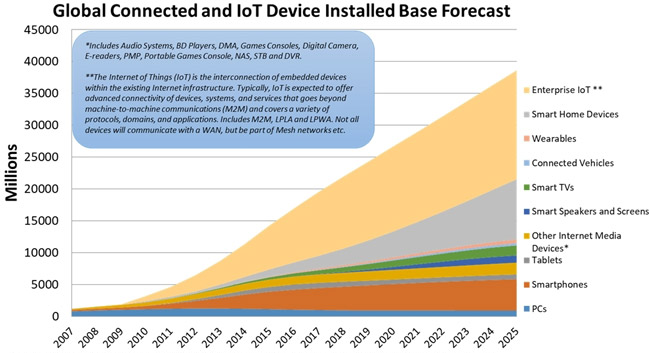
\includegraphics[width=0.75\textwidth]{forecast_iot_devices2}
  \caption{Strategy Analytics' forecast for the growth of IoT devices [Strategy Analytics]}
  \label{fig:forecast_iot_devices}
\end{figure}

Additionally, another key aspect in this new paradigm is the evolution of fibre optics technology which has resulted in the Internet backbone, allowing for the inter-connection of all these devices, fuelling our ever increasing demand for more data, re-shaping or creating entire markets such as online shopping or video on demand, and serving as the underlying infrastructure for mobile communication networks.

This momentum, however, comes with a new set of challenges. On one hand, having scores of electronic devices permanently active or even battery powered, requires us to come up with new ways to increase energy efficiency and develop disruptive battery technologies, if this reality is to become sustainable. On the other, the availability of more data, the sheer number of \emph{ad-hoc} connected nodes (the so called Internet of Things, IoT) and the mobile communications market in particular, have all called for vigorous new advances in the field of wireless protocols and architectures, sparking the interest both in academia and the industry. It is at the core of this ongoing revolution that software-defined radio (SDR) is making its mark.

%%%%%%%%%%%%%%%%%%%%%%%%%%%%%%%%%%%%%%%%%%%%%%%%%%%%%%%%%%%%%%%%%%%%%%%%%%%%%%%
\section{State of the Art}

The actual term \emph{software-defined radio} was coined by Joseph Mitola in a 1992 article entitled `Software radios - survey, critical evaluation and future directions' \cite{ntc92}, but some experiments have been conducted since the 70's, chiefly by military institutions in the United States (US) and Europe. Two early examples, the US Defence Advanced Research Projects Agency (DARPA) SpeakEasy project in 1991 and Joint Tactical Radio System (JTRS) in 1997 (shown in \autoref{fig:root_early_sdr_systems}), were both efforts to produce a unified radio system within the armed forces \cite{sdr_short_history}.

\begin{figure} [ht]
  \begin{subfigure}{.5\textwidth}
    \centering
    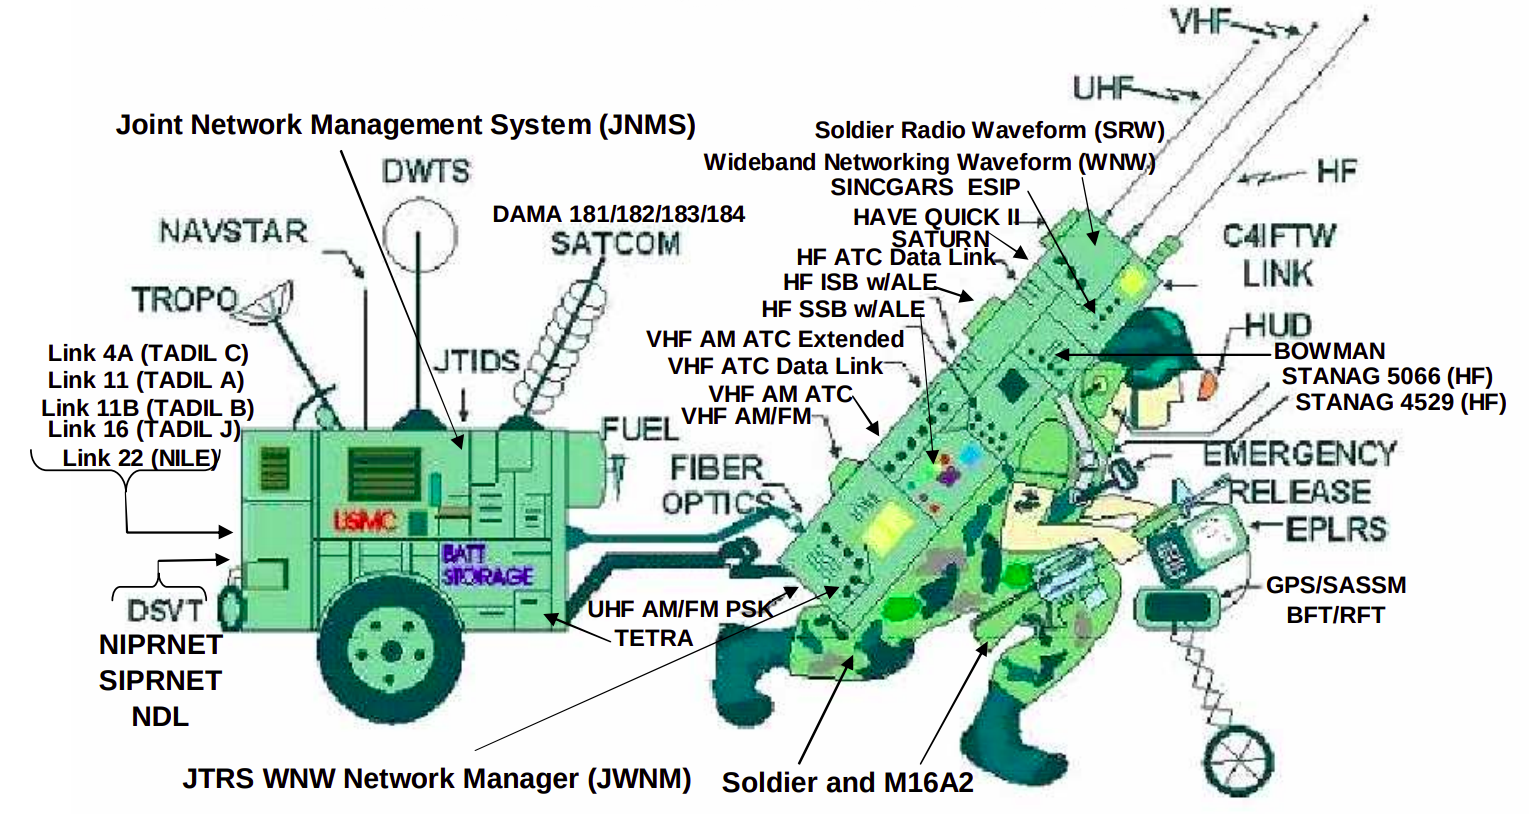
\includegraphics[width=.8\linewidth]{root_sdr_systems}
    \label{fig:root_sdr_systems}
  \end{subfigure}%
  \begin{subfigure}{.5\textwidth}
    \centering
    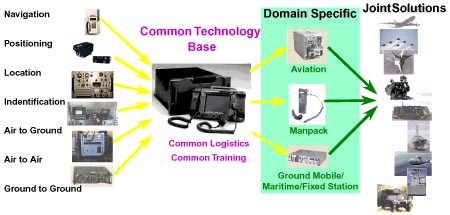
\includegraphics[width=.8\linewidth]{early_sdr_systems}
    \label{fig:early_sdr_systems}
  \end{subfigure}
  \caption[The JTRS multi-billion dollar program created by the US]{The JTRS was an ambitious multi-billion dollar program created by the US Department of Defence in 1997 to increase interoperability and waveform portability. It experienced difficulties, delays and  cost overruns leading to its cancellation in 2011. Despite that, it stimulated advances in SDR, both from manufacturers and other government agencies [\citeauthor{image:root_sdr_systems}].}
  \label{fig:root_early_sdr_systems}
\end{figure}

The increasing number of wireless protocols that have been developed nowadays however, such as Long Term Evolution (LTE) and beyond, for mobile communications; Zigbee, Bluetooth low energy (BLE) and Long Range (LoRa) for IoT; or new WiFi protocols for personal and machine-to-machine (M2M) communication, have brought the challenge to new levels. The need for a versatile transceiver design with the ability to handle several existing and future protocols, has never been bigger. In order to accomplish this task, one requires a flexible, re-configurable, and programmable framework. This is exactly the definition of SDR. A technology that is based on a software-defined approach, as opposed to hardware-based solutions. This means that features and functionalities, such as updating and upgrading through reprogramming, can be performed without having to replace the hardware on which they are implemented, opening the doors to the possibility of realizing multi-band and multi-functional wireless devices, effectively replacing hardware analogue blocks with software, and hardware description language (HDL) algorithms. Some examples of fields where SDR is being employed are:
\begin{itemize}
  \item Low-power IoT sensor nodes \cite{sdr_sensors}.
  \item Virtualized base stations controllers (BSCs) for mobile communication networks \cite{aict17}.
  \item Low-cost low earth orbit (LEO) satellite transceivers \cite{icssc16}.
  \item Academic research and educational tools, for example, in the fields of radio communications and digital signal processing (DSP) \cite{sdr_teaching}.
\end{itemize}

As far as SDR hardware is concerned, there are several options available today, ranging from low-end USB dongles with fairly limited RF and baseband performance, to high-end platforms which often include sophisticated signal correction hardware and algorithms, baseband computing power in the form of field-programmable gate arrays (FPGAs), and other advanced features, often bringing the price tag into the several thousands of US dollars.

There are quite a few key specifications to consider when characterizing the performance and capabilities of these platforms. A more incisive discussion into some of the possible SDR architectures, and their advantages and disadvantages, is presented in \autoref{chap:conceptual_overview}. As such, this section is limited to an overview of a few selected devices, representative of the spectrum of available options, focusing on some basic parameters, such as frequency range, bandwidth, sampling rate and resolution. These devices are the high-end professional level Universal Software Radio Peripheral (USRP) range from Ettus Research \cite{usrp_product_selector}, the open hardware and open source HackRF project from Great Scott Gadgets \cite{hackrf_one_product}, targeted at the academic/hobbyist audience, and the RTL-SDR \cite{rtlsdr_product}, an affordable Digital Video Broadcasting - Terrestrial (DVB-T) receiver with a RealTek chipset, that's been reverse-engineered by the community into a low-end SDR. A summary of the specifications for these devices, is laid out in \autoref{table:sdr_comparison}.

For the development of this thesis a HackRF One working as a transmitter, and an RTL-SDR as receiver, are used, and a more detailed description of these devices will be provided in \autoref{chap:demo_apps}.

\begin{table}[ht]
  \caption{Comparison of specifications from a few selected SDR platforms loosely spanning the spectrum of the currently available options}
  \label{table:sdr_comparison}
  \centering
  \begin{adjustbox}{width=1\textwidth}
  \begin{tabular}{>{\bfseries}l|c|c|c|c}
    \toprule
    \thead{Characteristics / Device} & \thead{USRP N210} & \thead{USRP B210} & \thead{HackRF One}  & \thead{RTL-SDR (RTL2832U)} \\
    \hline
    Full duplex                   & Yes                       & Yes                      & Half                    & No (only supports reception) \\
    Interface (throughput (Mbps)) & Gbit Ethernet (1000)      & USB 3.0 (5000)           & USB 3.0 (5000)          & USB 2.0 (480) \\
    MIMO                          & 2 TX - 2 RX               & 1 TX - 1 RX              & 1 TX - 1 RX             & 1 RX \\
    ADC/DAC resolution (bits)     & 14/16                     & 12/12                    & 8/8                     & 8 \\
    ADC/DAC sampling rate (Msps)  & 100/400                   & 61.4/61.4                & 20/20                   & 3.2 \\
    Frequency Range (GHz)         & 0-6                       & 0.07-6                   & 0.03-6                  & 0.024-1.776 \\
    Baseband hardware             & Spartan 3A-DSP 3400       & Spartan 6                & XC6SLX75                & CPLD \& 8051 + demod \\
    Cost [USD]                    & \multicolumn{1}{c|}{1750} & \multicolumn{1}{c|}{690} & \multicolumn{1}{c|}{300} & \multicolumn{1}{c}{10}
  \end{tabular}
  \end{adjustbox}
\end{table}

As far as SDR software is concerned, there are also quite a few alternatives available. Hardware developers tend to provide driver libraries that allow low-level interaction such as configuration, diagnostics, firmware upgrade and basic tx/rx (\emph{libhackrf} for the HackRF or \emph{librtlsdr} for the RTL-SDR, for example), and on top of that, SDR development frameworks have emerged. Two well-known frameworks are the PothosSDR project \cite{pothossdr_project} (which also includes the SoapySDR library \cite{soapysdr_project}) and the GNU Radio (GR) project \cite{gnuradio_project}. Since most of the projects are open source, the connections between them tend to assume more of a mesh layout than being completely separate. Further above these frameworks, sit SDR client programs that allow for a more high-level experience, such as GQRX (an SDR receiver powered by GNU Radio and the Qt graphical toolkit) and CubicSDR (an SDR receiver based on the SoapySDR platform). \autoref{fig:sdr_frameworks} is a block diagram loosely depicting some of the mentioned SDR libraries and client programs.

\begin{figure}[ht]
  \centering
  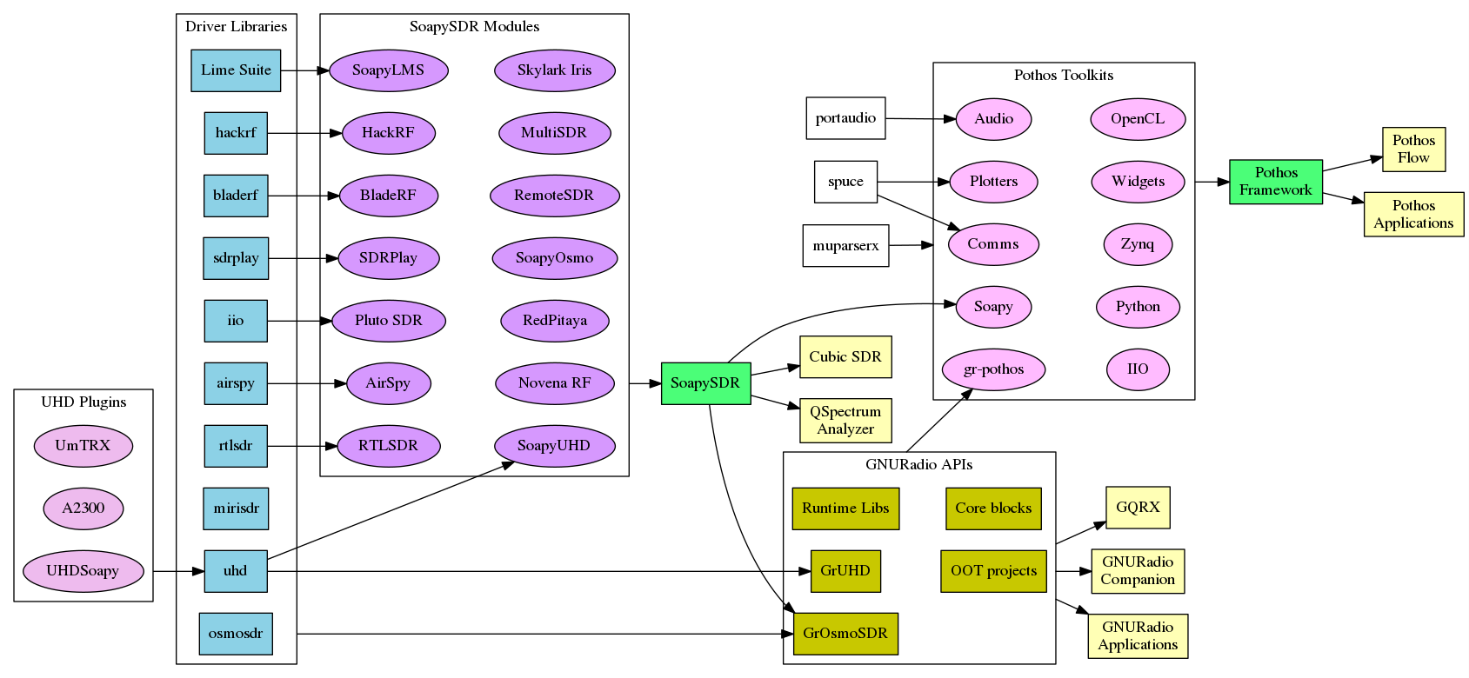
\includegraphics[width=\textwidth]{sdr_frameworks}
  \caption{Some of the most widely used SDR platforms and their inter-connections [\citeauthor{pothossdr_project}]}
  \label{fig:sdr_frameworks}
\end{figure}

A noteworthy exception is SDR\# (SDR Sharp), a modular client which depends only on low-level hardware libraries and not on any SDR framework, and can be seen in \autoref{fig:sdr_sharp}.

\begin{figure}[ht]
  \centering
  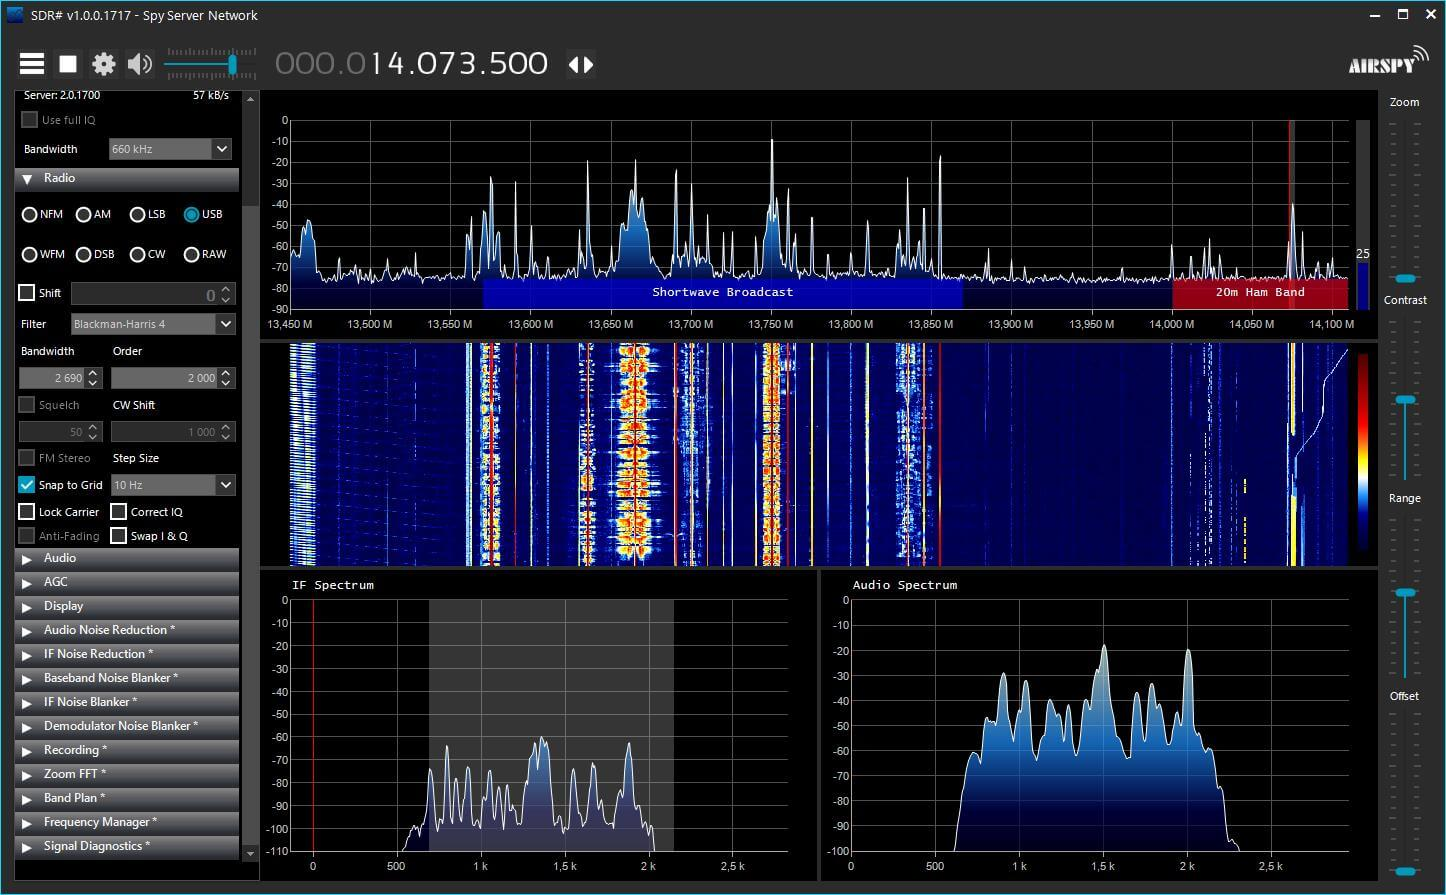
\includegraphics[width=0.85\textwidth]{sdr_sharp}
  \caption[SDR\# a popular SDR client]{SDR\# a popular SDR client developed in C\# by Airspy, who are also hardware SDR device manufacturers [\citeauthor{image:sdr_sharp_image}]}
  \label{fig:sdr_sharp}
\end{figure}

There is also some support within proprietary packages, such as MATLAB that provides wrappers for the USRP and RTL-SDR devices.

Finally, it is also common to encounter pure Python libraries for SDR research and experimentation. These can be simple packages that wrap low-level hardware libraries (such as \emph{pyrtlsdr} which is a Python wrapper of \emph{librtlsdr}), and which are often used in conjunction with other signal processing libraries such as \emph{NumPy} and \emph{SciPy}. Other types of libraries also exist that focus, not so much on the hardware interaction, but on SDR/DSP algorithms implementation (the \emph{komm} library \cite{komm_project} and the \emph{scikit-dsp-comm} library \cite{scikit-dsp-comm_project}, are good examples).

Of the mentioned frameworks, GNU Radio is very mature, flexible and exhaustive. An impressive amount of different technologies have been implemented, or at least prototyped, in it, such as Global System for Mobile Communications (GSM) \cite{gr-gsm} and Long-Term Evolution (LTE) \cite{gr-lte} receivers; several satellite technologies such as LEO and geosynchronous orbit (GEO) weather satellite demodulators \cite{meteor_m2_decoding}, and Cubesat receivers \cite{icssc16}; phase alternating line (PAL) and National Television System Committee (NTSC) decoders \cite{pal_decoder} \cite{ntsc_decoder}; 802.11a/g/p WiFi and 802.15.4 Zigbee transceivers \cite{wime_project}, frequency modulation (FM) transceivers \cite{gnuradio_wbfm_receiver}, among many others. For this reason, it has been chosen to implement the demonstration applications in this thesis. A more detailed description of the GNU Radio SDR framework is presented in \autoref{chap:demo_apps}.

%%%%%%%%%%%%%%%%%%%%%%%%%%%%%%%%%%%%%%%%%%%%%%%%%%%%%%%%%%%%%%%%%%%%%%%%%%%%%%%
\section{Objectives}
\label{sect:objectives}
The main objective of this thesis is to create a software framework of DSP algorithms that can demonstrate the potential applications of SDR as an educational tool for digital communication systems, in the academic context.

This will be achieved, first by creating a library that includes implementations of several key algorithms relevant to signal processing in the context of telecommunications, such as digital modulators, FIR interpolators/decimators, channel models and impairments (for example, an additive white gaussian noise (AWGN) channel model, phase/frequency offset, IQ imbalance and DC offset), frequency and phase correction techniques, clock synchronization, forward error correction (FEC) algorithms, among others. The library will be developed in Python, which provides a good balance between speed of development and performance. It also makes it easy to re-use in other environments, such as GNU Radio (GR), which natively support Python. This framework will constitute the backbone of the project and can, in the future, be extended with other algorithm implementations, as learning exercises for fellow students/users in DSP subjects. Several key best practices will be used (such as unit testing framework and code documentation) so as to introduce users to the importance of these requirements in a software project lifecycle, in order to keep a fairly high standard of code quality and documentation.

The library will also be accompanied by a set of \emph{Jupyter notebooks}, that will be created to demonstrate the workings and usage of the developed modules. This is aimed at, not only showing the concepts, but also highlighting the benefits of the Jupyter framework for rapid prototyping and proof of concept demonstrations.

On top of this library, and as means of direct application demonstration, two GNU Radio applications will be developed. The first is a \emph{wideband frequency modulation} (WBFM) demodulator, optimized for embedded systems (GR already includes a WBFM implementation \cite{gnuradio_wbfm_receiver} and a brief comparison with the proposed algorithm will be presented). The main idea is to demonstrate how SDR applications have the potential to replace legacy analogue systems with relative ease. The second application will be a \emph{phase-shift keying} (PSK) transceiver. This will also be developed in GR, but instead of implementing the algorithms directly in GR blocks, it will make full use of the Python library and simply create thin wrappers in GR. Requisites for this PSK transceiver include BPSK and QPSK modulations, channel impairments corrections, and both propagated and radiated real-time environment functionality with actual hardware deployment (as opposed to only performing offline file processing in simulation environment).

%%%%%%%%%%%%%%%%%%%%%%%%%%%%%%%%%%%%%%%%%%%%%%%%%%%%%%%%%%%%%%%%%%%%%%%%%%%%%%%
\section{Thesis Structure}

This thesis is organized in five chapters.

\autoref{chap:introduction} provides a brief overview of the evolution of wireless communication systems, with a focus on the reasons leading to the large increase of connected devices in recent years. It then introduces the concept of SDR systems with a brief historical background, and discusses in more detail the state of the art, with respect to both hardware and software solutions.

\autoref{chap:conceptual_overview} presents a theoretical description of a few of the most commmon SDR architectures. An initial introduction defines the main blocks in an SDR system (radio frequency (RF) section, intermediate frequency (IF) section and signal processing section), and then a more detailed discussion of each section is presented. In each of them, the general aspects of each architecture along with their advantages and disadvantages, and main applications are discussed. In order to better understand the implications of each architecture, it's important to be aware of key RF concepts and parameters which are widely used to evaluate the dynamic performance of SDR systems (and RF communication systems in general). Towards this end, an initial section on these topics is presented, prior to discussing the SDR architectures.

\autoref{chap:sksdr_lib} describes the algorithms developed for the DSP/SDR library (the library is named SKSDR after \emph{science kit SDR}). This library constitutes the backbone of the project and is later used for SDR demonstration applications. Each algorithm is discussed in detail in a separate section. In addition to the detailed theoretical explanation, a summary of the API is also provided, as well as usage examples, both using IPython (Python REPL interpreter) and Jupyter notebooks.

\autoref{chap:demo_apps} is dedicated to the SDR demonstration applications. An initial section describes, in more detail, the hardware used and the GNU Radio platform, giving some examples of simple GR flowgraphs. \autoref{sect:WBFM_Receiver_with_alternate_algorithm} starts by describing the specifications of a typical FM broadcast system. It then describes the standard WBFM demodulation implementation in GR and proceeds to explain in depth, the alternative proposed algorithm. There are many techniques for FM demodulation but they generally fall within a set of 4 classes of algorithms. These are identified and briefly described, and both the GR standard implementation and the alternative implementation are framed within them. After this, the PSK transceiver is also presented in detail in \autoref{sect:psk_transceiver} with both the GR flowgraphs design and execution being demonstrated, together with some result analysis.

Finally \autoref{chap:conclusions} concludes the thesis, including a discussion on achieved results, key takeaways and future work.


\chapter{Conceptual Overview}
\label{chap:conceptual_overview}
This chapter presents a conceptual overview of SDR systems. \autoref{fig:sdr_block_diagram} shows a block diagram of a typical SDR system both from transmitter and receiver sides.
\begin{figure}[ht]
  \centering
  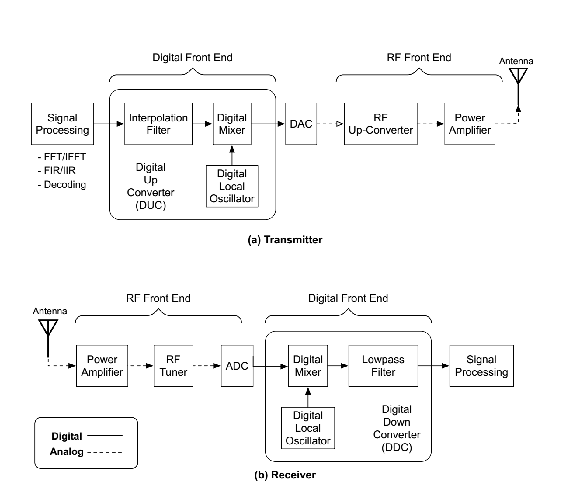
\includegraphics[width=0.75\textwidth]{sdr_block_diagram}
  \caption{Generic SDR architecture [\citeauthor{DBLP:journals/corr/abs-1804-06564}]}
  \label{fig:sdr_block_diagram}
\end{figure}

An SDR transceiver typically consists of the following components: signal processing unit, digital front end, analogue RF front end, and an antenna.
\begin{enumerate}
  \item Antenna: Several types of antennas can be used to cover a wide range of frequency bands \cite{communications_receivers}, depending on the tuning and protocol capabilities of the SDR equipment. A frequent option in LEO satellite reception is the use of rotating antennas to follow the satellite's path. Other technologies that can be very useful in SDR systems are the so called `intelligent' or `smart' antennas that can use mobile tracking (i.e beam-forming capability), and/or interference cancellation (sometimes known as self-healing) \cite{rf_dig_sig_processing} \cite{review_tech_sdr}.

  \item RF front end: This is the RF circuitry responsible for transmitting and receiving the signal at various carrier frequencies. As a minimal structure, it's composed of a local oscillator (LO), a mixing section, and a power section (a power amplifier (PA) in the transmission path and a low-noise amplifier (LNA) in the receiver path). Real-world devices typically include other blocks such as power detectors and filters.
  \begin{enumerate}
    \item In the transmission path the analogue signal is mixed with a local oscillator (LO) signal to produce the RF signal at the preset frequency. It is then amplified using a power amplifier (PA) and transmitted. Advanced techniques such as digital pre-distortion (DPD) or envelope tracking, can be used to maximize output power while maintaining linearity in the PA. Other components that are typically part of this section are impedance matching networks, diplexers and RF filters such as surface acoustic wave (SAW) filters to reduce interference and comply with regulations like, for example, transmission masks.
    \item In the receiver the signal is connected to the RF front end using impedance matching circuitry to avoid signal reflections and ensure maximal power transfer. It is then fed to a low noise amplifier (LNA), which is usually placed close to the antenna, in order to amplify the incoming signal and maximize the SNR. This amplified signal is mixed with the LO signal and converted directly to baseband, or to an intermediate frequency (IF) in the case of heterodyne architectures\cite{tech_radio_handbook}. Other components that can also exist are power detectors for gain control, and RF filters to suppress interference in the form of image frequencies.
  \end{enumerate}

  \item Analogue-to-digital (ADC) and digital-to-analogue (DAC) conversion: The DAC is responsible for producing the analogue signal to be transmitted, from the digital samples. On the receiver side, the ADC performs the inverse operation by converting the continuous-time signal to a discrete-time, binary-coded signals. The devices can operate at baseband or IF, depending on the SDR architecture. ADC performance can be described by various parameters \cite{adc_survey} \cite{digital_frontend_sdr} including: signal-to-noise-and-distortion ratio (SINAD), effective number of bits resolution (ENOB), spurious-free dynamic range (SFDR), among others. These parameters are discussed in more detail, in \autoref{sect:radio_performance_and_impairment}.

  \item Digital front end: The digital front end executes some tasks traditionally implemented in the analogue domain. Two of its main functions are\cite{digital_frontend_sdr}:
  \begin{enumerate}
    \item  Sample rate conversion. Frequently, baseband blocks operate at a much lower frequency than the ADC/DAC devices. This requires an upsampling and interpolation operation (increasing the sample rate), or a decimation and downsampling operation (reducing the sample rate). The decimation filter in the receiver is typically matched to the transmitter's interpolation filter, in order to reduce additive noise. This is known as \emph{matched filtering} and is a common technique to design optimum receiving filters \cite{communication_systems_carlson}.
    \item Channelization. This includes up/down conversion in the transmitter and receiver side. For example in digital IF applications, the digital up converter (DUC) translates the baseband signal to IF, using digital mixer and a numerically-controlled oscillator (NCO). The DAC that is connected to the DUC then converts the digital IF samples into an analogue IF signal. In the receiving side the ADC converts the IF signal into digital samples and these are fed into the digital down converter (DDC) which is composed of a digital mixer and a NCO to obtain baseband digital signal from the IF signal.
  \end{enumerate}

  \item Signal processing: This block is responsible for the signal processing operations, such as forward error correction (FEC) encoding/decoding, interleaving/deinterleaving, modulation/demodulation, and scrambling/descrambling. Another crucial block is the fast Fourier transform (FFT) and inverse FFT (IFFT), which can be used in modulation (for example in orthogonal frequency-division multiplexing (OFDM) systems \cite{ofdm_baseband_receiver}) and other algorithms that operate in the frequency domain (for example, frequency offset compensation algorithms). The signal processing block implementation needs to run on top of hardware circuitry that is able to process these signals very efficiently. Depending on the system specifications these hardware platforms can include general purpose processors (GPPs), graphics processing units (GPUs), digital signal processors (DSPs), field programmable gate arrays (FPGAs) and application-specific integrated circuits (ASICs). Often the most computing-intensive operations can be deployed in dedicated hardware such as an FPGA core. In \autoref{sect:dsp_realizations} a more detailed discussion is presented on the aforementioned hardware platforms and the various design approaches.
\end{enumerate}

The next sections will be dedicated to describing each of the aforementioned SDR sections in more detail (with the exception of the antenna). Prior to that, in \autoref{sect:radio_performance_and_impairment}, a description is made of some general concepts related to radio performance and impairments, which are important to understand both the characteristics of each SDR architecture, and the results from the applications developed in \autoref{chap:demo_apps}. This section also discusses important parameters related to the ADC/DAC devices. \autoref{sect:sdr_system_architecture} then describes some of the possibilities for SDR topologies in terms of the RF front end and digital front end sections, listing their advantages and disadvantages. These topologies are broadly grouped into three groups:
\begin{enumerate}
  \item RF sampling: architectures which sample the RF signal directly, without first converting to an intermediate frequency or to baseband.
  \item IF sampling: architectures which first convert the signal to an intermediate frequency (usually in the tens of megahertz) and then perform sampling.
  \item Baseband sampling: Architectures which convert the signal to baseband (also known as 0 Hz or DC), and then perform sampling.
\end{enumerate}


Finally, \autoref{sect:dsp_realizations} discusses some of the most common options employed for realization of the signal processing stage (the core of the SDR), describing the advantages and disadvantages of each one.

%%%%%%%%%%%%%%%%%%%%%%%%%%%%%%%%%%%%%%%%%%%%%%%%%%%%%%%%%%%%%%%%%%%%%%%%%%%%%%%
\section{Radio Performance and Impairments}
\label{sect:radio_performance_and_impairment}

This sections describes some RF performance concepts and parameters, which are important when understanding the different SDR architectures, and when evaluating the performance of the developed algorithms and applications.

One of the most important parameters is the \emph{signal-to-noise ratio} (SNR) which defined as the ratio of the total signal power to the total noise power:
\begin{align}
  \text{SNR} = \frac{S}{N} = \left(\frac{S_{rms}}{N_{rms}}\right)^2
\end{align}
where
\begin{itemize}
  \item $S$ = Input signal power, in Watt
  \item $N$ = Noise power, in Watt
  \item $S_{rms}$ = Root-mean-square (RMS) amplitude of input signal
  \item $N_{rms}$ = RMS amplitude of noise
\end{itemize}

\noindent Power, noise and SNR are often expressed in logarithmic units, rather than linear units:
\begin{align}
  \text{SNR(dB)} = 10\log(SNR) =  10\log(S) - 10\log(N) = S\text{(dBm)} - N\text{(dBm)}
\end{align}

When analysing SDR systems, two of the most important components are ADC and the DAC. To analyse these, a common set of parameters is typically employed by manufacturers, which facilitates comparison between devices (although sometimes insufficient testing conditions information, such as signal frequency range, bandwidth and repetition, makes it difficult to obtain a trustworthy comparison). One of these parameters is the \emph{total harmonic distortion} (THD), which is defined as the ratio of the RMS value of the fundamental signal to the equivalent RMS of its harmonics (generally, only the first 5 harmonics are significant). THD of an ADC is usually measured in dBc and generally specified with the input signal close to full-scale, although it can be specified at any level.
\begin{align}
  \text{THD} = \frac{S_{rms}}{D_{rms}} = \frac{S_{rms}}{\sqrt{H_{1_{rms}}^2+H_{2_{rms}}^2+H_{3_{rms}}^2+H_{4_{rms}}^2+H_{5_{rms}}^2}}
\end{align}
where $D_{rms}$ represents distortion introduced by the harmonics.

\emph{Spurious free dynamic range} (SFDR) is another parameter, defined as the ratio of the RMS value of the input signal to the RMS value of the worst spurious signal regardless of where it falls in the frequency spectrum. The worst spur may or may not be a harmonic of the original signal. SFDR is an important specification in communications systems because it represents the smallest value of signal that can be distinguished from a large interferer. SFDR can be specified with respect to full-scale (dBFS) or with respect to the actual signal amplitude (dBc). \autoref{fig:sfdr_plot} illustrates how SFDR can be measured.

\begin{figure}[ht]
  \centering
  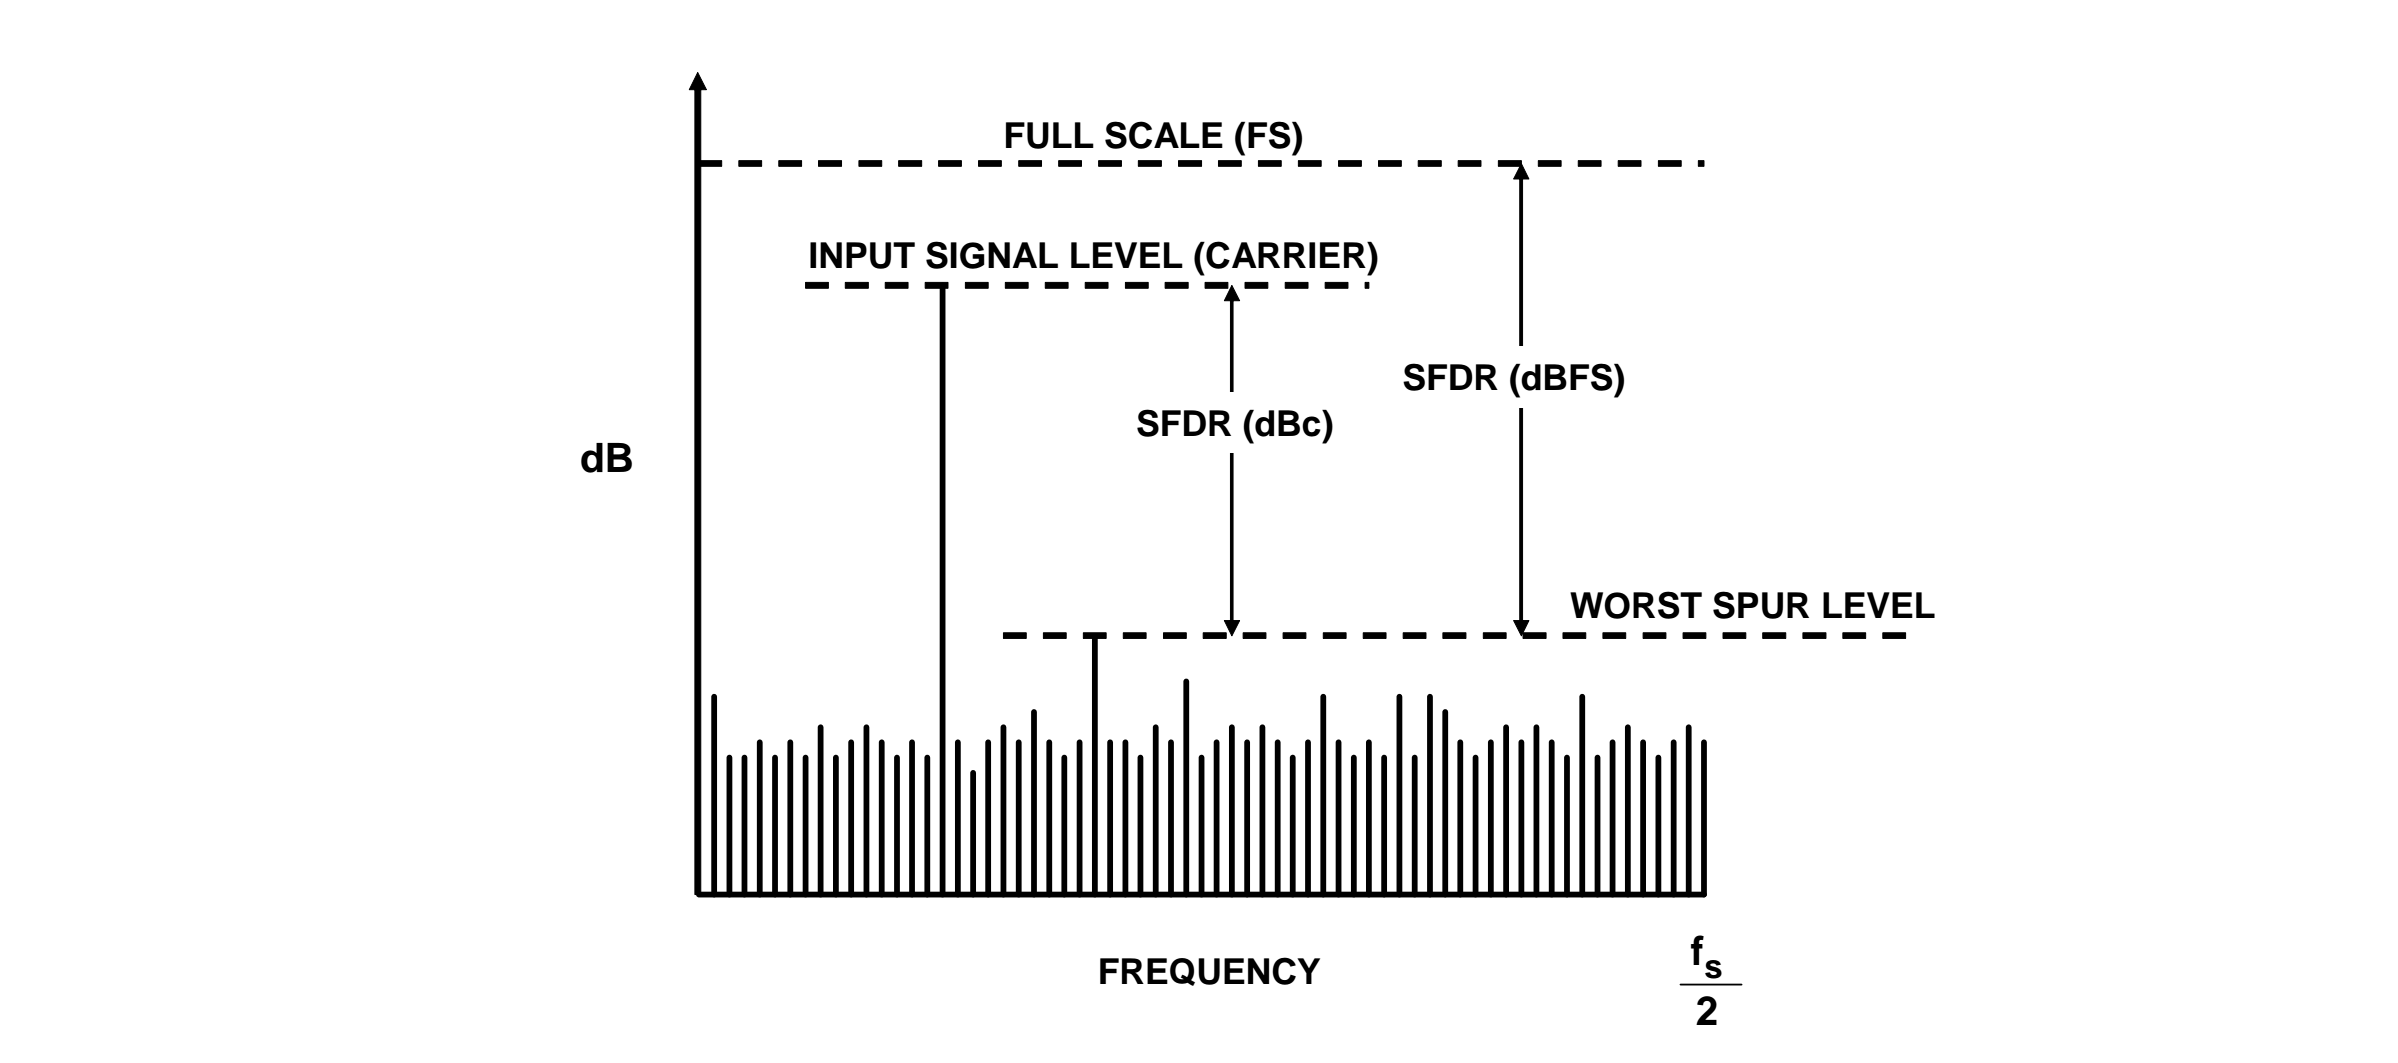
\includegraphics[width=\textwidth]{sfdr_plot}
  \caption{Spurious Free Dynamic Range [\citeauthor{understand_sinad}]}
  \label{fig:sfdr_plot}
\end{figure}

Finally the \emph{signal to noise and distortion ratio} (SINAD) is defined as the ratio of the RMS value of the input signal to the RMS value of all other spectral components including harmonics (but excluding DC):
\begin{align}
  \text{SINAD} = \frac{S_{rms}}{D_{rms}+N_{rms}}
\end{align}

SINAD is a good indicator of the dynamic performance of ADCs since it includes all components that make up noise and distortion. This parameter can also be related to the number of bits of the ADC using the theoretical ideal model of an ADC which assumes that only quantization noise exists and that it approximates AWGN \cite{improve_adc_res}:
\begin{align} \label{eq:SNR_ADC_dB}
  \text{SINAD(dB)} = (6.02 \cdot N_b) + 1.76
\end{align}
where $N_b$ is the number of bits of the ADC. It's important to note that \eqref{eq:SNR_ADC_dB} assumes a full-scale input signal as well. Finally, oversampling and averaging can be employed to reduce the in-band noise and hence increase the SINAD. In this case $N_b$ in \eqref{eq:SNR_ADC_dB} is replaced by the \emph{effective number of bits} (ENOB). Without going into the full detail, one can state a simple, but useful, rule of thumb:

\begin{displayquote}
  \emph{Each doubling of the sampling frequency will lower the in-band noise by 3 dB, and increase the resolution of the measurement by $1/2$ bit.}
\end{displayquote}

Note that whenever one is looking at a signal in the frequency domain, that's been obtained through an FFT, it's important to take into account the effects of the window used, namely the apparent attenuation caused by the signal not being contained within a single FFT bin (an effect known as \emph{scalloping loss}). Full analysis in beyond the scope of this thesis but can be consulted in \cite{harris_windows}.

SNR (or SINAD) can also be related to digital domain parameters. Closely related to the SNR is the $E_s$/$N_0$ parameter which is the ratio between the symbol energy and the noise spectral density. This parameter can be defined (in dB), and related to the SNR, as follows:
\begin{align}
  \frac{E_s}{N_0} (\text{dB}) & = 10\log_{10}\left(S\frac{T_{s}}{(N/B_n)}\right) \nonumber \\
                              & = 10\log_{10}\left(T_{s}F\left(\frac{S}{N}\right)\right) \nonumber \\
                              & = 10\log_{10}\left(\frac{T_{s}}{T}\right) + \text{SNR(dB)}
\end{align}
where
\begin{itemize}
  \item $T$ = Sampling period, in seconds
  \item $T_s$ = Symbol period, in seconds
  \item $S$ = Input signal power, in Watt
  \item $N$ = Noise power, in Watt
  \item $B_n$ = Noise bandwidth, in Hz $= F = 1/T$.
  \item $F$ = Sampling frequency, in Hz
\end{itemize}

$E_s/N_0$ can also be expressed in terms of the closely related ratio of the bit energy to the noise spectral density $E_b/N_0$ as
\begin{align}
  \label{eq:esn0}
  E_s/N_0 = E_b/N_0 + 10\log_{10}(k)
\end{align}
where $k$ is the number of information bits per symbol. Note that $k$ depends on the size of the modulation and the code rate of an error-control code. As an example, using a $4/7$-rate code and 16-QAM modulation, $k$ is $\log_2(16) (4/7) = 16/7$, the product of the number of bits per symbol and the code rate.

Finally, and perhaps most important, is the notion of channel capacity famously introduced by Shannon \cite{shannon_capacity}. The information capacity of a channel of bandwidth $B$ (in Hz) with AWGN noise of power spectral density $N_0/2$ is given by
\begin{align}
  C = B\log_{2}\left(1+\frac{P}{N_0 B}\right)
\end{align}
where $P$ is the average transmitted power.

Note that the dependency on bandwidth $B$ is \emph{linear} but the dependency on SNR, $\frac{P}{N_0 B}$, is \emph{logarithmic}. This leads to an insightful conclusion:

\begin{displayquote}
  \emph{To increase the capacity of a communications systems it's easier to expand the bandwidth of the channel than to increase the transmitted power, for a given noise variance}.
\end{displayquote}

From this results it's possible to derive the familiar plots that relate SNR (or $E_b/N_0$) to bit-error rate (BER) which provide a very useful visual representation of the performance of digital modulations. \autoref{fig:PSK_BER_curves} shows a typical $E_b/N_0$ to BER curve for PSK modulations.

\begin{figure}[ht]
  \centering
  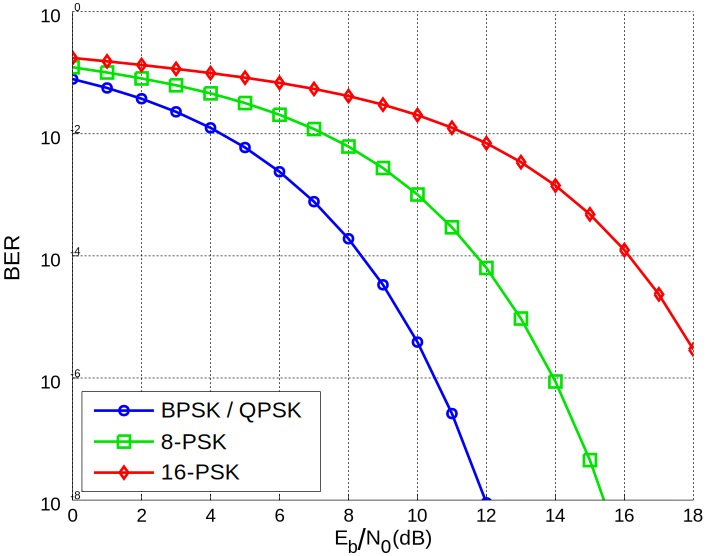
\includegraphics[width=0.75\textwidth]{PSK_BER_curves}
  \caption{Bit-error rate curves for BPSK, QPSK, 8-PSK and 16-PSK, AWGN channel [\citeauthor{image:ber_curve}]}
  \label{fig:PSK_BER_curves}
\end{figure}

Other parameters which are important in RF performance analysis, and are widely used for example in characterising PAs, are the 1-dB compression point (P1dB) and the third-order intercept point (IP3).

An amplifier usually provides a constant gain over a specific frequency range, giving a linear relation between input power and output power. For example, if the gain of an amplifier is 10 dB, then a 1 dBm input signal will result in an 11 dBm output signal. As the input power level increases, there comes a point where the output power of the amplifier no longer increases by the gain value (i.e., the amplifier output power starts to saturate). The P1dB is the output power level at which the gain decreases 1 dB from its constant value \cite{p1db}. Once an amplifier reaches its P1dB it goes into compression and becomes a non-linear device, producing distortion. P1dB is one of the most important specifications for power amplifiers. \autoref{fig:p1db} shows an illustration of the P1dB.

\begin{figure}[ht]
  \centering
  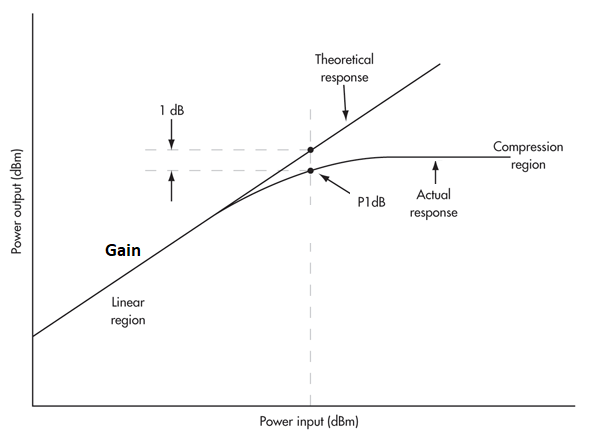
\includegraphics[width=0.6\textwidth]{p1db}
  \caption{1-dB compression point [\citeauthor{p1db}]}
  \label{fig:p1db}
\end{figure}

IP3 is a figure of merit based on the idea that the device nonlinearity can be modelled using a low-order polynomial, derived by means of Taylor series expansion around a small deviation\cite{iip3}. The third-order intercept point relates nonlinear products caused by the third-order nonlinear term to the linearly amplified signal. Its definition can be based on a single tone input or two-tone input.
\begin{itemize}
  \item Based on harmonics: The device is tested using a single input tone. The nonlinear products caused by $n$-th-order nonlinearity appear both at the input tone frequency and at $n$ times it's frequency.
  \item Based on intermodulation products: The device is fed with two sine tones one at $f_1$ and one at $f_2$.  When you cube the sum of these sine waves you will get sine waves at various frequencies including $(2f_2-f_1)$ and $(2f_1-f_2)$.  If $f_1$ and $f_2$ are large but very close together then $(2f_2-f_1)$ and $(2f_1-f_2)$ will be very close to $f_1$ and $f_2$. This two-tone approach has the advantage that it is not restricted to broadband devices and is commonly used for radio receivers.
\end{itemize}
For example, for an input $s_i=S_1 \cos(\omega_1 t)$ and a transfer function given by $s_o=a_1 s_i + a_2 (s_i)^2 + a_3 (s_i)^3$, the cubic term generates
\begin{equation}
  (S_1)^3 (\cos(\omega_1 t))^3 = (S_1)^3 (\frac{3}{4})\cos(\omega_1 t)+\frac{1}{4})\cos(3\omega_1 t))
\end{equation}
The intercept point can then be obtained graphically (\autoref{fig:iip3}) by plotting the output power versus the input power both on logarithmic scales (e.g., decibels). Notice that on a logarithmic scale, the function $x^n$ translates into a straight line with slope of $n$. Therefore, the linearly amplified signal will exhibit a slope of $1$. A third-order nonlinear product will increase by 3 dB in power when the input power is raised by 1 dB. The point where the curves intersect is the intercept point which can be read from the input or output power axis (IIP3 or OIP3).

\begin{figure}[H]
  \centering
  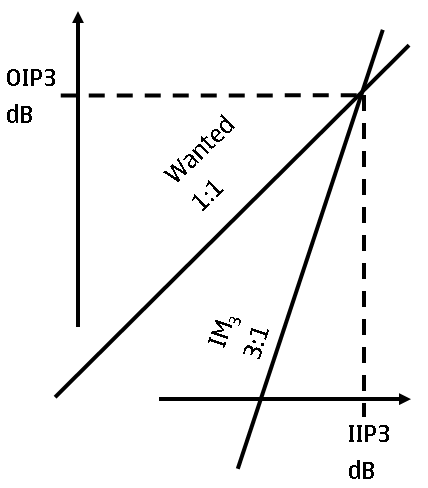
\includegraphics[width=0.4\textwidth]{iip3}
  \caption{Third-order intercept point [\citeauthor{iip3}]}
  \label{fig:iip3}
\end{figure}

Other important parameters, specific to quadrature systems, are \emph{IQ amplitude imbalance} and \emph{IQ phase imbalance}, which have to do with different gain and matching in the I and Q paths of a quadrature system. These will be discussed in more detail in \autoref{sect:sdr_system_architecture}.

%%%%%%%%%%%%%%%%%%%%%%%%%%%%%%%%%%%%%%%%%%%%%%%%%%%%%%%%%%%%%%%%%%%%%%%%%%%%%%%
\section{SDR System Architectures}
\label{sect:sdr_system_architecture}

This section covers some possible architectures in SDR systems, highlighting the main advantages and disadvantages of each one.

\subsection{Ideal SDR System}

The ideal SDR system (shown in \autoref{fig:ideal_sdr}) is one where the entire processing logic is encompassed within the DSP subsystem and the RF section simply needs to amplify and transmit/receive the signal. In this architecture the signal coming from/to the DAC/ADC is already at RF frequency so needs no further up/down conversion. Also, note the ADC and DAC include the anti-alias and reconstruction filters.

\begin{figure}[H]
  \centering
  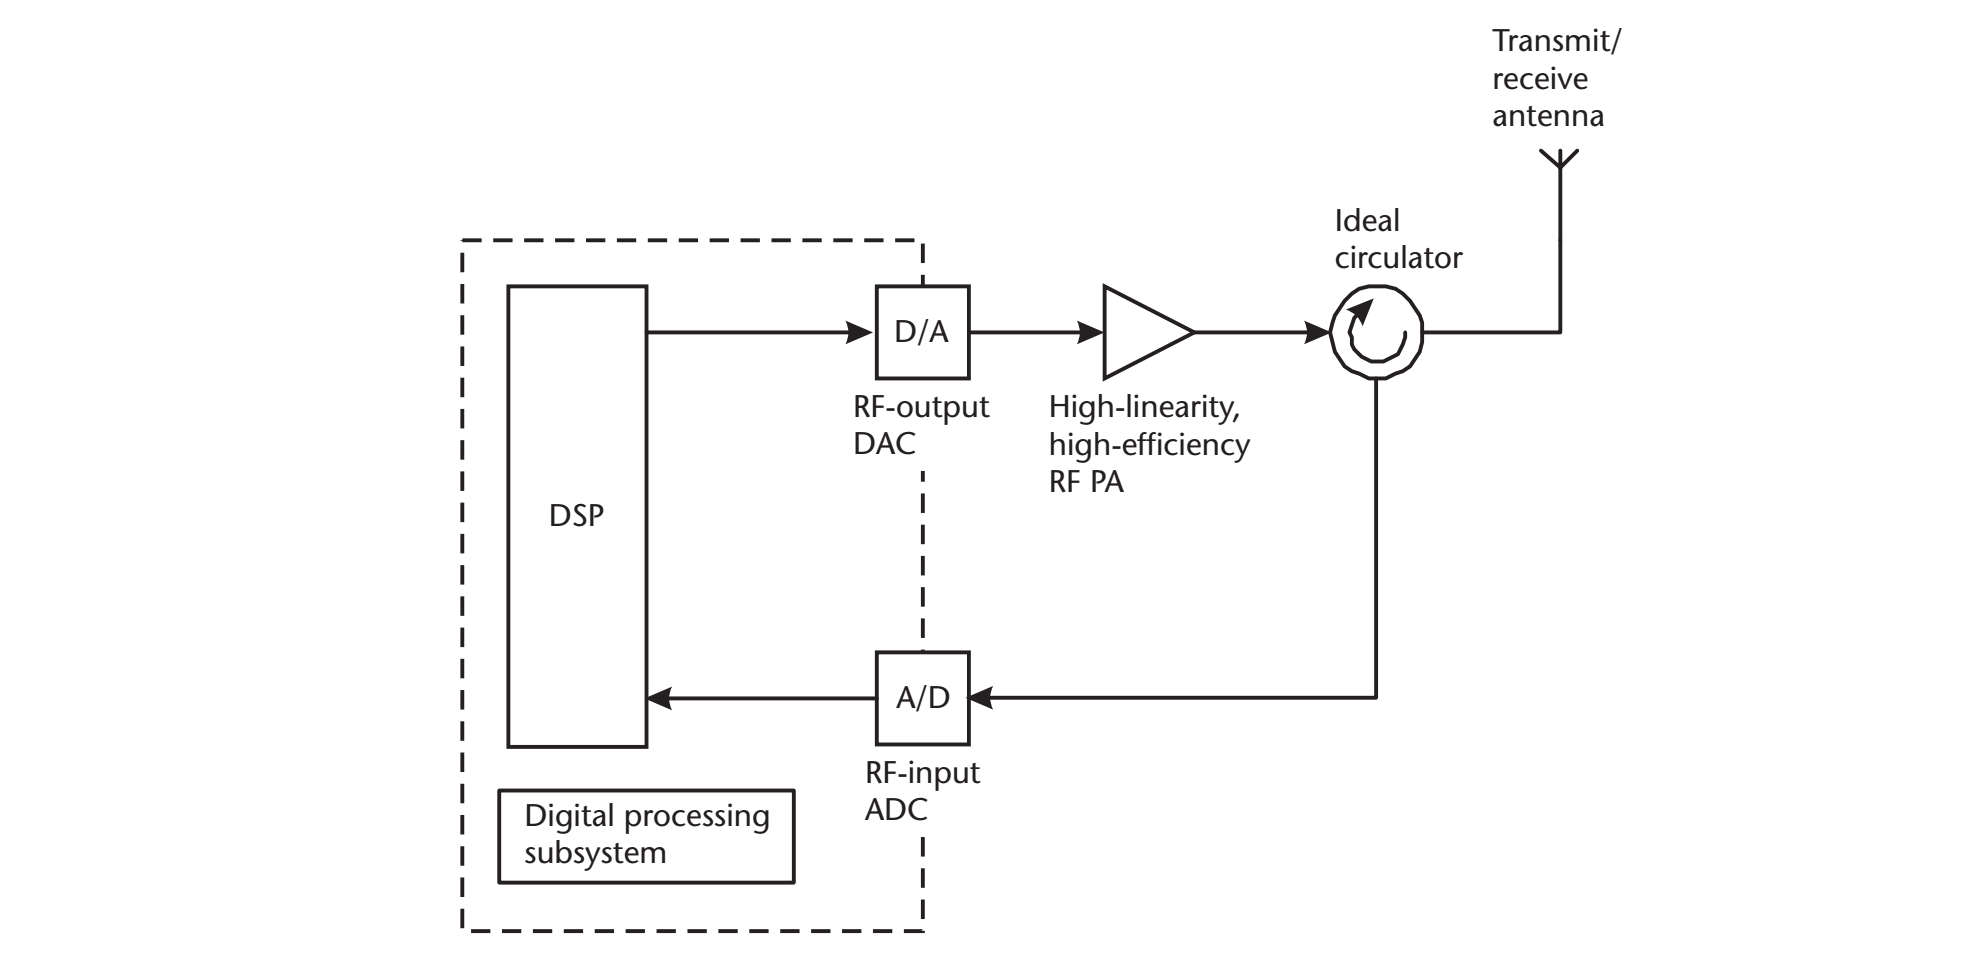
\includegraphics[width=\textwidth]{ideal_sdr}
  \caption[An ideal SDR system]{An ideal SDR system where the entire signal processing (including up/down conversion to the desired RF frequency) is achieved in the DSP subsystem [\citeauthor{rf_bb_techniques_sdr}]}
  \label{fig:ideal_sdr}
\end{figure}

Some of the clear advantages are:
\begin{itemize}
  \item Extremely simplified RF chain.
  \item Elimination of most of the analogue RF related problems such as DC offset, gain/phase imbalance in IQ systems, phase noise from oscillators, among others.
  \item Very high level of flexibility for implementing new protocols and/or when the processing power needs to be upgraded.
\end{itemize}

Unfortunately, technology has not evolved enough to make these systems cost effective. Their chief disadvantage is the fact that they rely on state-of-the-art high-speed ADC/DAC which are very expensive and power demanding (see \autoref{fig:adc12dj2700_power}), compared to a traditional up/down conversion RF chain (even considering the layout engineering effort involved in traditional RF chain design). Note that even if bandpass sampling is employed (which relaxes the sampling frequency requirements of the converters) the large analogue bandwidth necessary at the ADC input (often in the GHz range) is unavoidable if broadband is a requisite. Additionally, the realization of the anti-aliasing filter, which needs to provide sufficient attenuation in the stopband, while being tuned across the entire frequency range, is extremely challenging. As such, this architecture is necessarily reserved for systems where there are no budget restrictions. An RF sampling ADC characteristics page from a well-known vendor is shown in \autoref{fig:adc12dj2700_buy}. In this figure one can observe the very high sampling rate and input bandwidth, among other parameters. Note the full-scale input voltage of the ADC ($V_{FS}$) is just 0.8 V\textsubscript{pp}.

\begin{figure}[H]
  \centering
  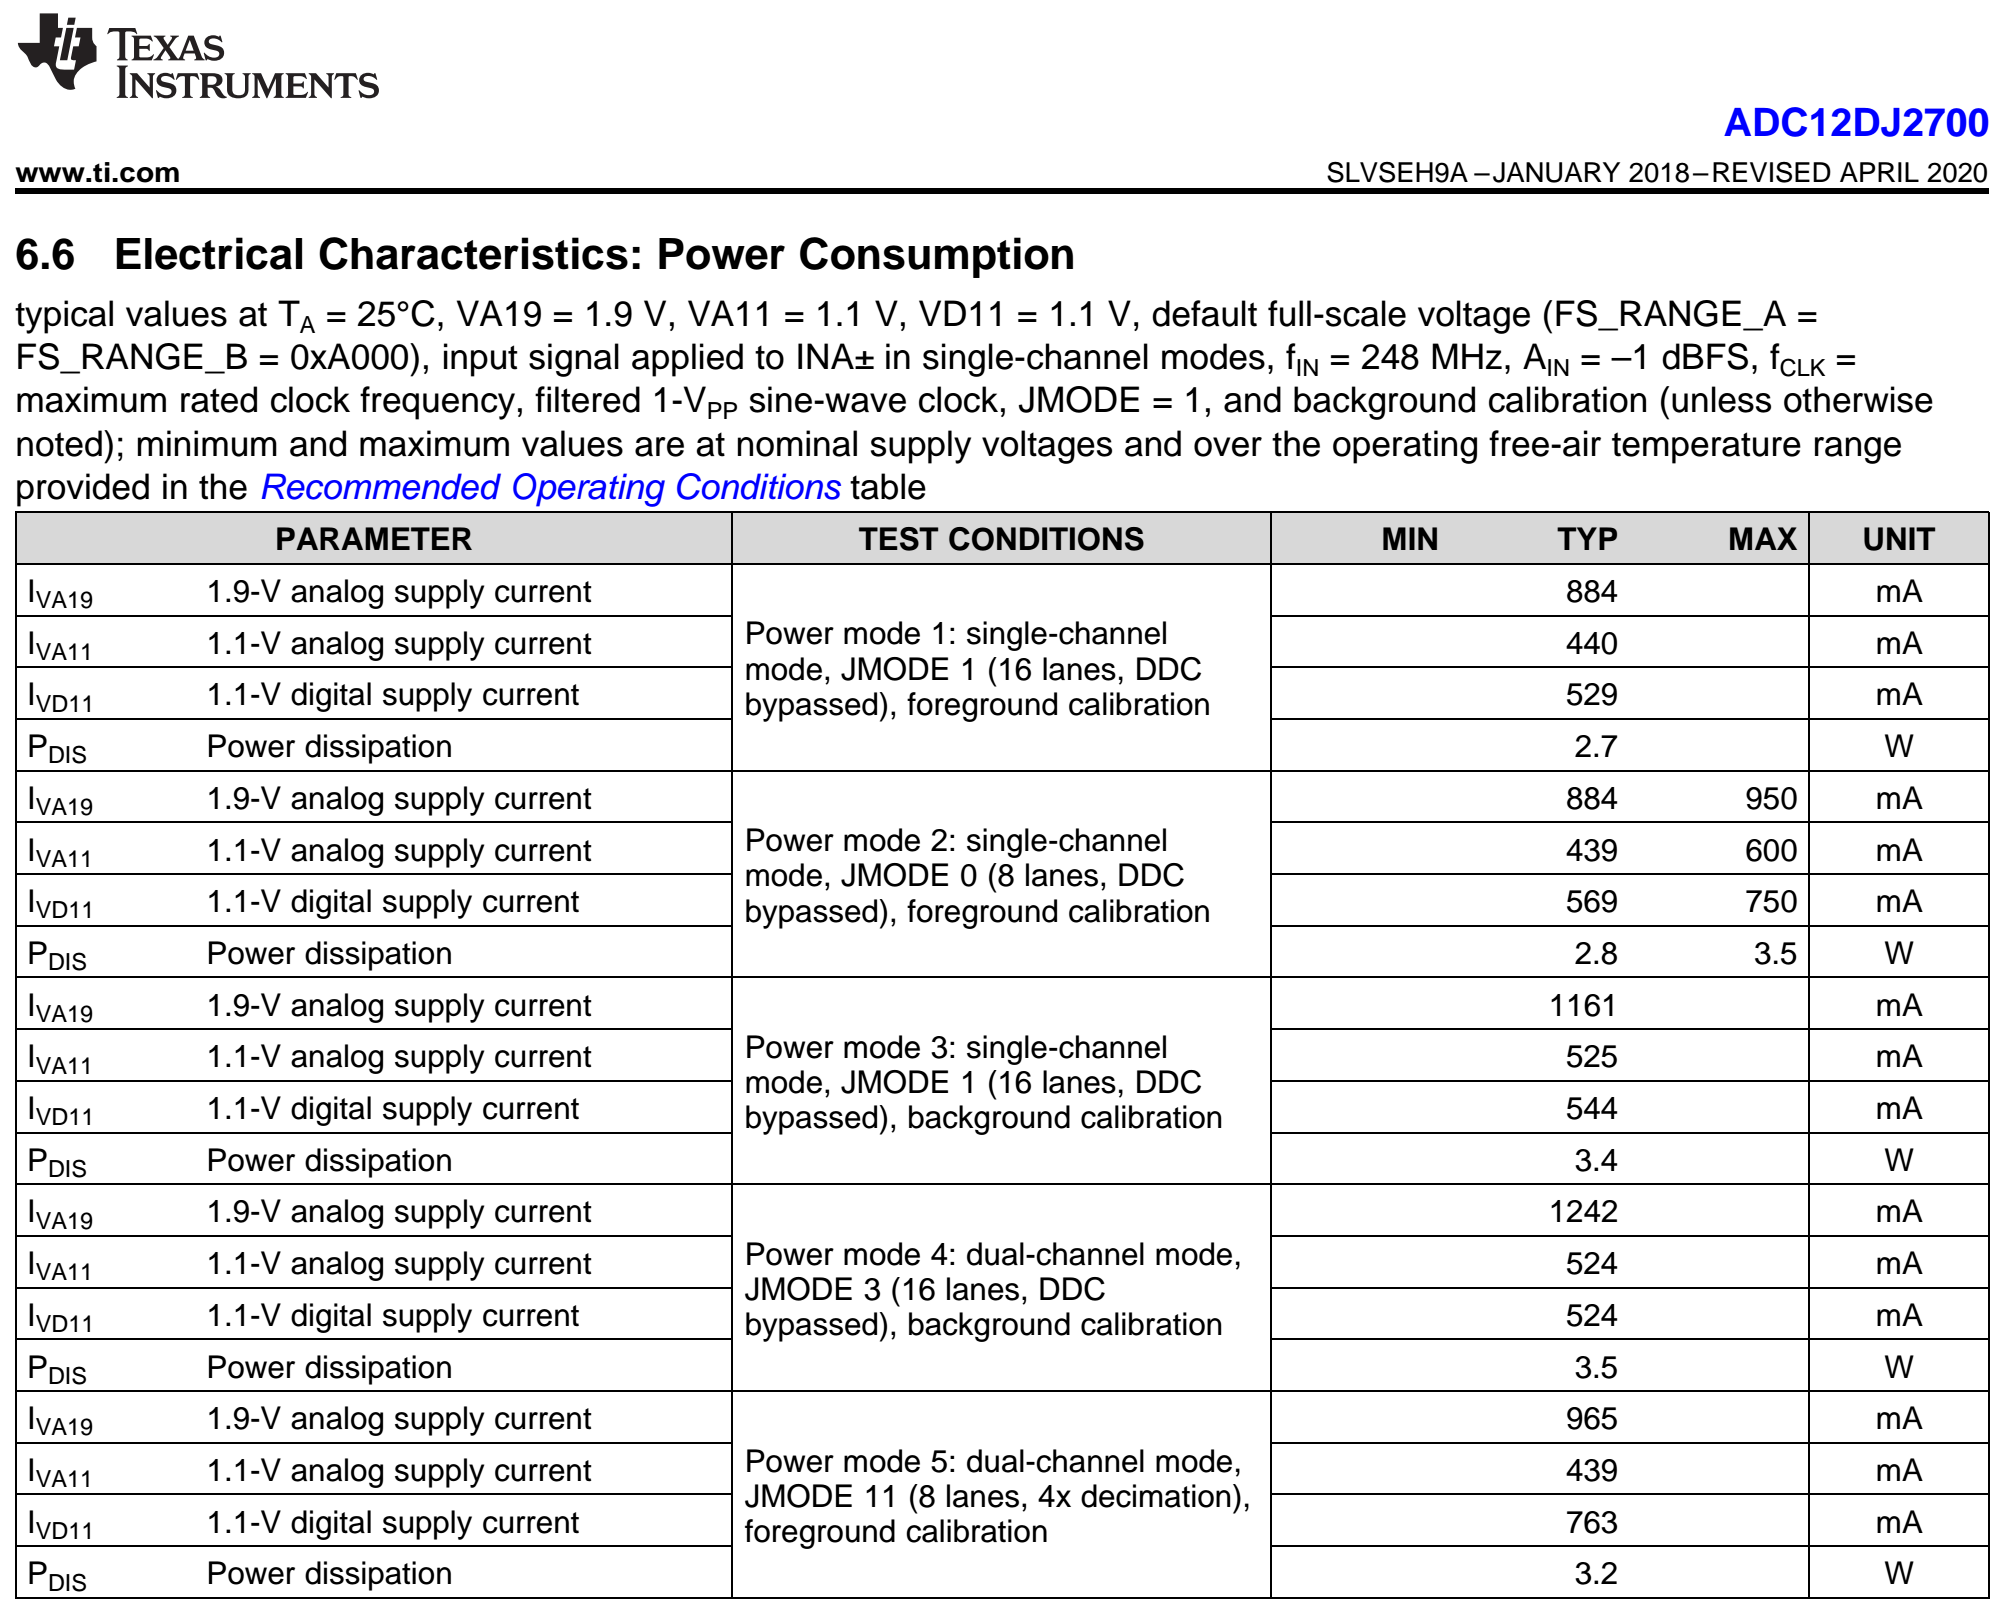
\includegraphics[width=\textwidth]{adc12dj2700_power}
  \caption[TI ADC12DJ2700 power consumption]{An extract from the TI ADC12DJ2700 datasheet, showing the power consumption of the device (from 2.7 W to 3.5 W depending on power mode)}
  \label{fig:adc12dj2700_power}
\end{figure}

\begin{figure}[H]
  \centering
  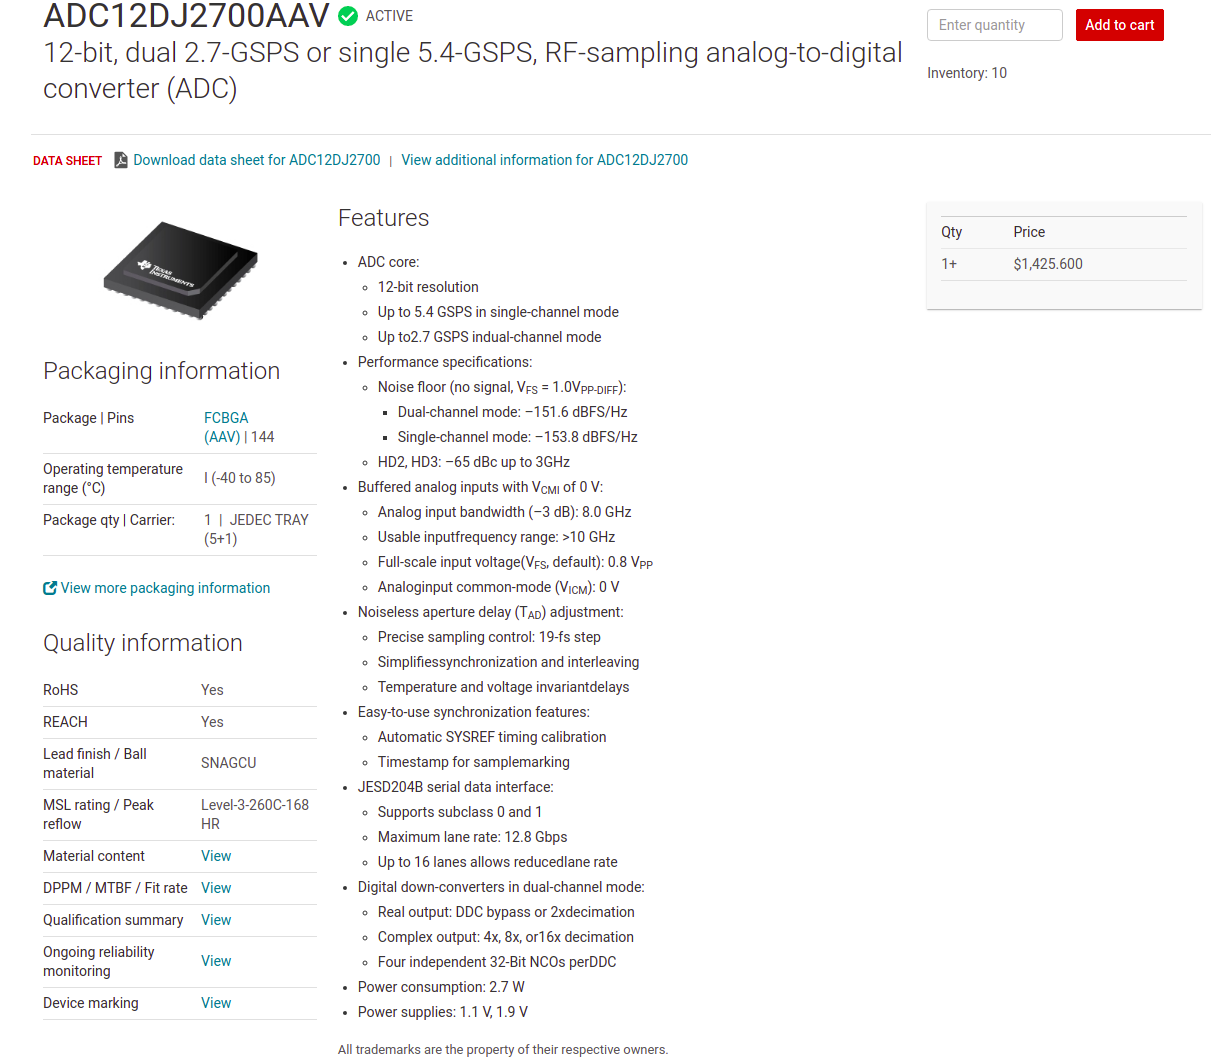
\includegraphics[width=\textwidth]{adc12dj2700_buy}
  \caption[TI ADC12DJ2700 specifications]{The TI ADC12DJ2700, a dual 2.7 GSPS, 12-bit RF sampling ADC which costs \$1425.60 per unit}
  \label{fig:adc12dj2700_buy}
\end{figure}

\subsection{Analogue Quadrature Receiver Architecture}
\label{sect:analogue_quadrature_receiver_architecture}

An alternative approach is seen in \autoref{fig:analog_quadrature_receiver} (only the receive path is shown for simplicity).

\begin{figure}[ht]
  \centering
  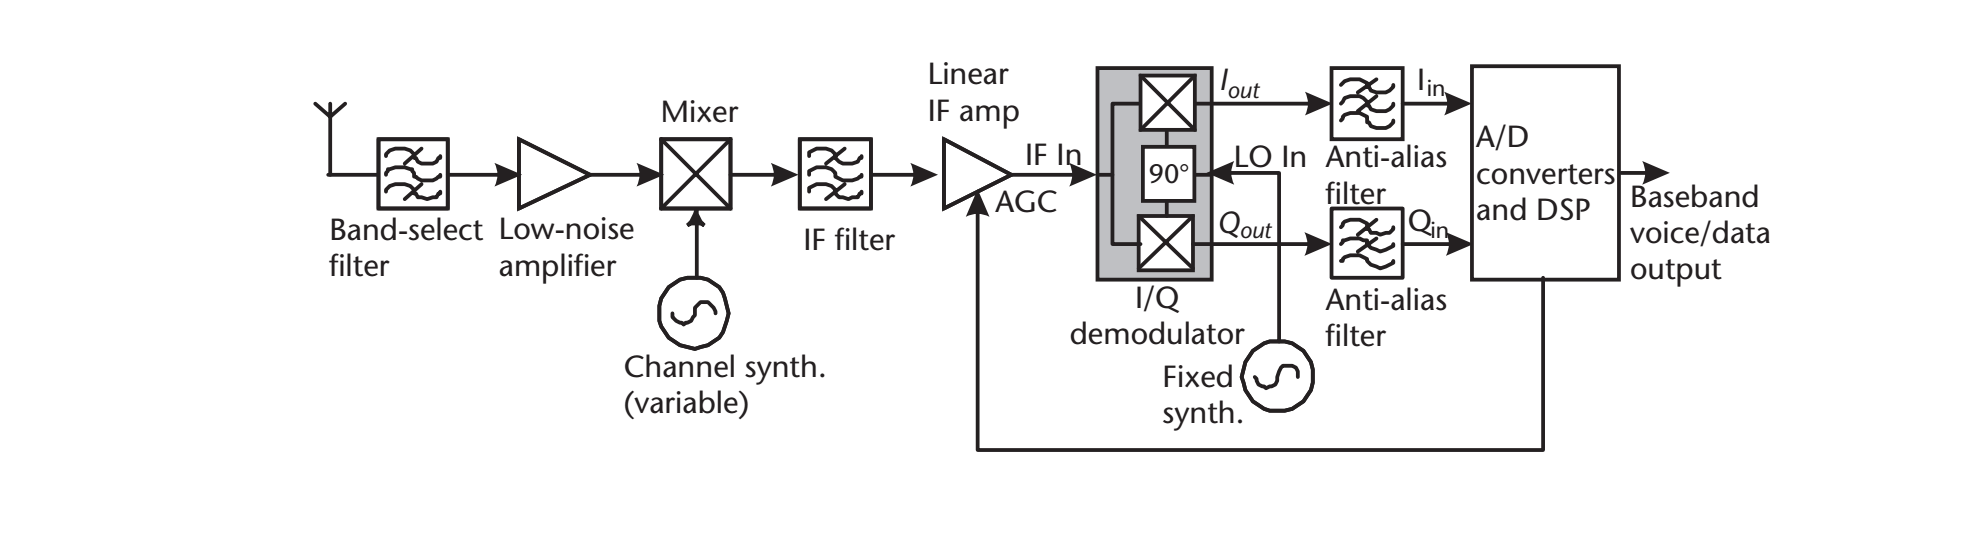
\includegraphics[width=\textwidth]{analog_quadrature_receiver}
  \caption[Analogue quadrature receiver design]{Analogue quadrature receiver design. A common implementation of SDR where the signal modulation and coding is performed in the DSP but the up/down conversion is achieved in the analogue domain [\citeauthor{rf_bb_techniques_sdr}].}
  \label{fig:analog_quadrature_receiver}
\end{figure}

In this case the RF chain needs to amplify and down-convert to IF. After that, the IF filter obtains the desired channel and then the signal is further down-converted to baseband, where the signal is low-pass filtered before being sampled by the ADC. The DSP finally performs the signal demodulation and decoding tasks such as constellation mapping and error correction decoding. The advantages in this architecture are:
\begin{itemize}
  \item Common and well understood architecture. For example, the IF section mitigates the DC offset problem caused by finite isolation between the input and the oscillator mixer ports (common problem in zero IF (ZIF) architecture, see \autoref{sect:zif_arch}).
  \item Transmit/receive path and ADC/DAC with more relaxed requirements can be implemented with relatively low-cost devices. ADC/DAC needs only to accommodate the baseband bandwidth and sampling frequency. Notice that it's becoming more common for the ADC/DAC blocks to include the anti-alias and reconstruction filters in one monolithic package, still maintaining low cost.
  \item Potential for implementing techniques such as oversampling to increase the ENOB and improve SNR.
\end{itemize}

The price to pay is:
\begin{itemize}
  \item Complex analogue path could lead to a slew of problems, especially if care is not taken in the layout phase. Potential for IQ gain and phase imbalance which need to be corrected.
  \item  Multi-stage amplification and filtering leads to the need to a complex mixed signal automatic gain controller (AGC) implementation where the DSP needs to control the analogue section gains in a feedback configuration to avoid saturation (note the figure shows the AGC controlling only the IF amplifier, but more often than not, it needs to control the whole chain, specially the LNA). Multiple oscillators can lead to strict clock requirements and complex architectures for coherent detection.
  \item Changes is system requirements such as different protocols and/or frequency ranges could potentially implicate a full hardware system re-design.
\end{itemize}

\subsection{Digital IF Receiver Architecture}

Perhaps a compromise between the two previous approaches is the \emph{Digital IF } architecture shown in \autoref{fig:digital_if_receiver}. In this realization, the analogue chain ends at the IF stage. The ADC samples directly at IF frequency and the conversion to baseband is performed in software by the DSP, together with the remaining demodulation, error correction and any other signal processing tasks. The IF frequency needs to be sufficiently high to allow channel selection (for example 10 MHz being the minimum requirement, for 3GPP WCDMA, for example), but sufficiently low that it results in achievable A/D and DSP processing bandwidth. This compromise is currently around the 10-50 MHz region, but continues to increase as A/D converter technology evolves.

\begin{figure}[H]
  \centering
  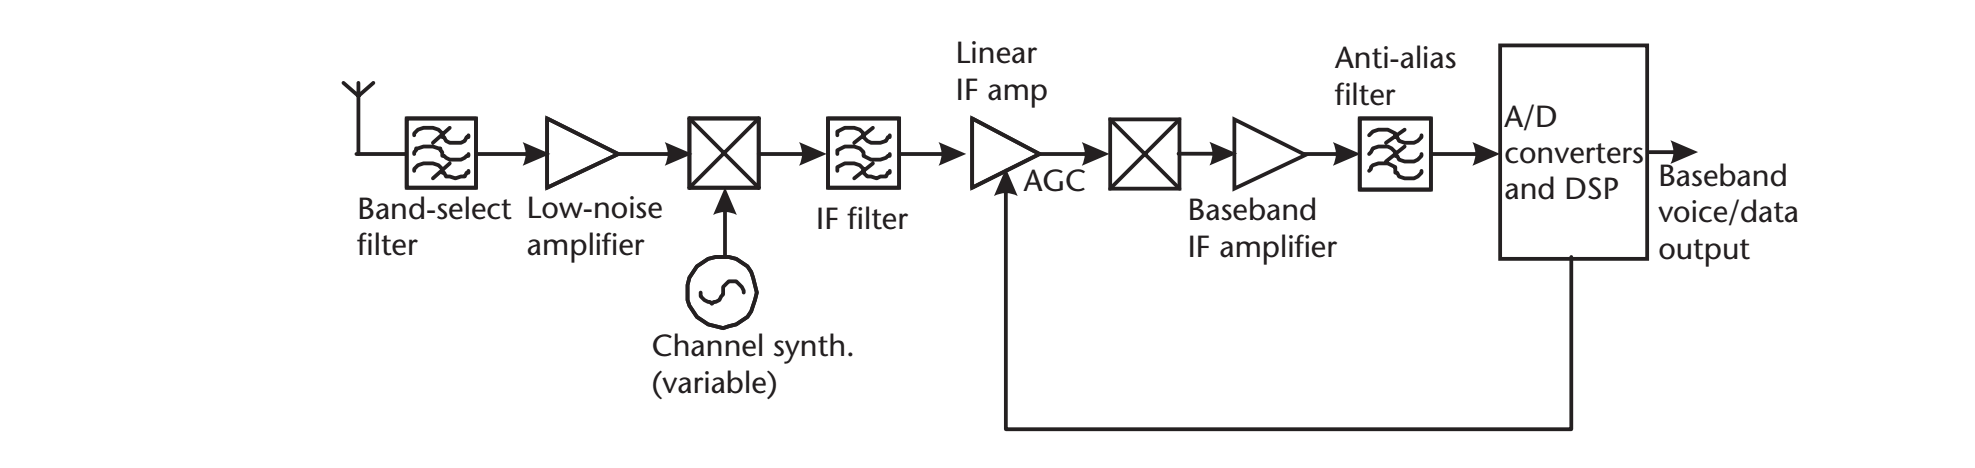
\includegraphics[width=\textwidth]{digital_if_receiver}
  \caption[Digital IF architecture]{Digital IF architecture. The analogue chain ends at the IF section. The ADC sample directly at the IF frequency and the downconvertion is then implemented in the DSP [\citeauthor{rf_bb_techniques_sdr}].}
  \label{fig:digital_if_receiver}
\end{figure}

There are some interesting advantages to this architecture:
\begin{itemize}
  \item Analogue section is confined to a single downconversion stage. The quadrature downconversion can be implemented in the DSP simply by mixing with quadrature numerically-controlled oscillator (NCO) running at $f_s/4$. This can be achieved by multiplying the digital IF samples by the periodic sequences [1, 0, -1, 0] for the in-phase channel and [0, -1, 0, -1] for the quadrature channel, therefore eliminating the problems mentioned in the analogue quadrature receiver architecture. This technique is shown in \autoref{fig:digital_quadrature_demod}.
  \item Simpler considerations for clocks and less analogue blocks to calibrate and control, lead to less requirements and complexity in the firmware.
  \item Potential for power consumption benefits  by having fewer analogue blocks and a simplified power saving logic.
\end{itemize}

The main disadvantages are:
\begin{itemize}
  \item Increased bandwidth necessary at the ADC to sample at IF, therefore possibly limiting other techniques such as oversampling.
  \item High-Q RF filtering section (typically a SAW filter) that needs to reject the image frequency at $f_c \pm f_i$.
\end{itemize}

\begin{figure}[ht]
  \centering
  
\includegraphics[width=\textwidth]{digital_quadrature_demod}
  \caption{Conceptual process of a digital quadrature demodulator [\citeauthor{rf_bb_techniques_sdr}]}
  \label{fig:digital_quadrature_demod}
\end{figure}

\subsection{Zero IF (ZIF) Receiver Architecture}
\label{sect:zif_arch}

In this architecture (also known as a \emph{homodyne receiver}), proposed by Colebrook in 1924 \cite{homodyne}, there is no IF stage, so the signal is directly converted to/from baseband. An example of this technique is shown in \autoref{fig:zif_receiver}.

\begin{figure}[H]
  \centering
  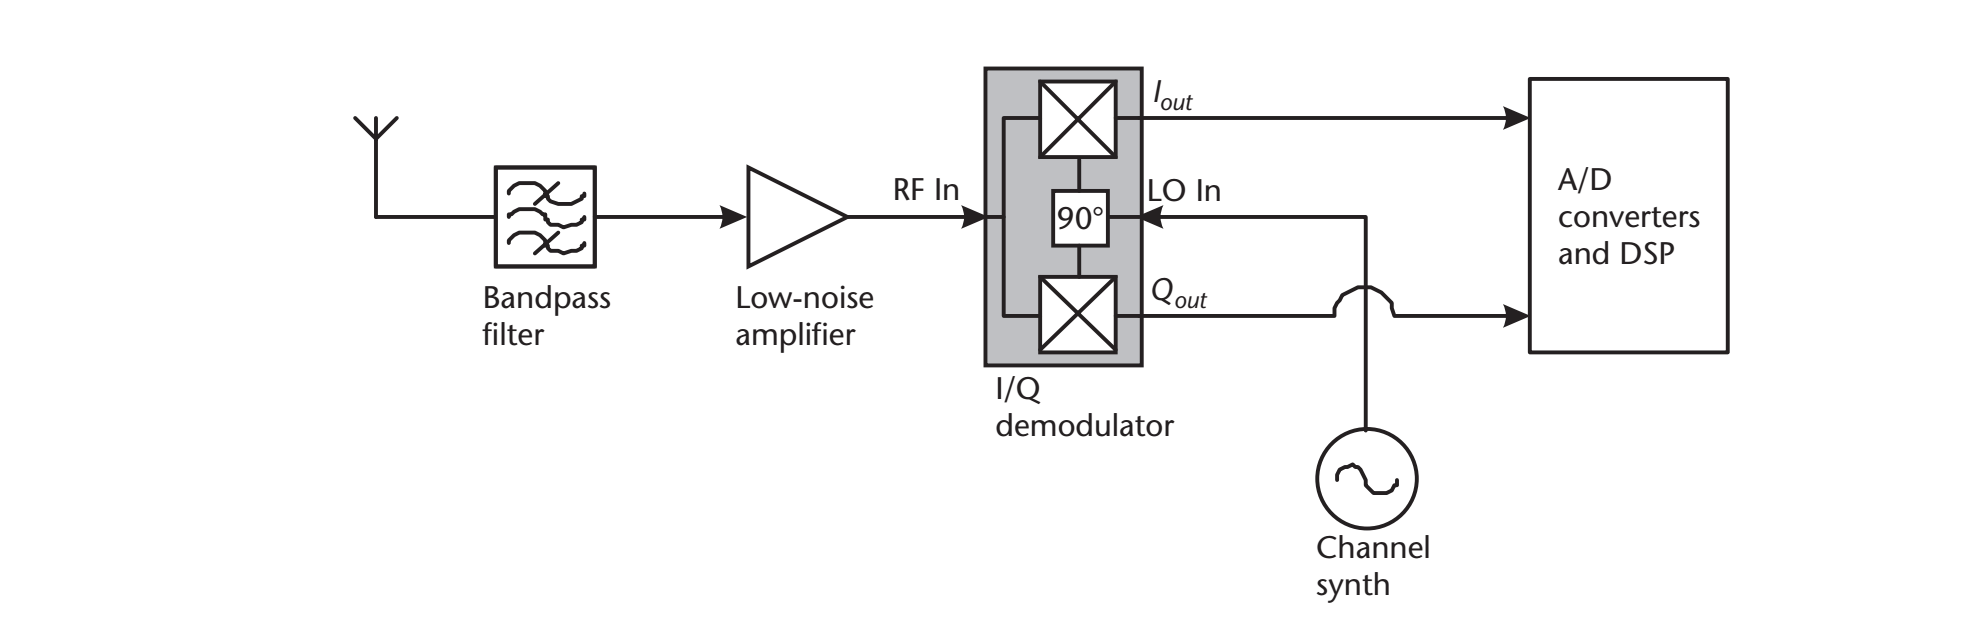
\includegraphics[width=\textwidth]{zif_receiver}
  \caption{Direct Conversion also known as Zero IF Architecture [\citeauthor{rf_bb_techniques_sdr}]}
  \label{fig:zif_receiver}
\end{figure}

This is potentially a very attractive option for the following reasons:
\begin{itemize}
  \item The use of digital filters allows for the implementation of better channel selection filters than could be implemented with analogue IF. In particular, linear-phase filtering is possible, an important property for digital modulation schemes.
  \item The image frequency is in-band and hence the required image-rejection is considerably reduced.
  \item Only a single local oscillator is required, which is advantageous compared to heterodyne systems.
  \item No IF filter is required, hence saving cost and PCB footprint.
\end{itemize}

It does, however, have a number of fundamental problems:
\begin{itemize}
  \item A well designed broadband quadrature network is required, to avoid IQ gain and phase imbalance.
  \item A DC offset appears at the centre of the baseband channel in I and Q and is usually quite high in level with respect to the weaker signals which the receiver may be required to demodulate. This is a consequence of the LO signal leaking to the input port of the mixer and mixing with itself thus appearing at DC. It is caused by finite isolation between LO and input ports in the mixer.
  \item The use of a baseband IF results in problems with low-frequency noise appearing at the centre of the channel ($1/f$ noise).
\end{itemize}

%%%%%%%%%%%%%%%%%%%%%%%%%%%%%%%%%%%%%%%%%%%%%%%%%%%%%%%%%%%%%%%%%%%%%%%%%%%%%%%
\section{Signal Processing Realizations}
\label{sect:dsp_realizations}

SDR signal processing sections are implemented through employing various types of hardware platforms, such as GPPs, GPUs, DSPs, and FPGAs. Each of these has their unique list of challenges. Some of these challenges are:
\begin{itemize}
  \item Making sure there are development tools that allow for an efficient design and implementation process
  \item Efficiently using the the available computational power
  \item Maintaining a low power consumption
  \item Keeping the overall equipment and tools cost low
\end{itemize}

\subsection{GPP}
GPPs are clock-driven and register-based and, for this reason, are capable of different processing functions \cite{microprocessors_and_microcontrollers}. This flexibility makes them tailored to a large number of applications, removing the need for developing application specific circuits. GPPs also allow access to high-level programming languages and well-known frameworks and software packages, making them popular within the scientific community. From the performance point of view, GPPs are being enhanced, due to technological advances in semiconductor technology \cite{lin2014a}, and also to parallelism techniques  in multi-core GPP \cite{ulversoy2010a}. Despite these advances, GPPs cannot match dedicated application-specific platforms for high-throughput computing with real-time requirements, precisely because of their sequential processing model \cite{kamal2003a}. The fact that the GPP often has to switch between different tasks when coupled with an operating system (OS), compromises its performance and can quickly reach saturation with frames becoming corrupted and being discarded. In addition, some protocols require predictable performance in order to guarantee meeting timing constraints. However, conditional branch instructions in GPPs instruction sets lead to out-of-order execution, which makes this difficult to achieve.

In recent years scientists have began to experiment with coupling GPPs wityh GPUs. The latter are specifically designed to handle graphics-related tasks and as such they efficiently process large blocks of streaming data in parallel. This naturraly leads to a model where the act as co-processors for demanding operations, with the GPP typically acting as the control processor. SDR platforms comprised of both GPPs and GPUs have higher processing power but also lower power efficiency than dedicated architectures such as FPGAs (due mostly to the GPP. E.g., GPP's power efficiency is about 9 GFLOPS/W for single precision, compared to 20 GFLOPS/W for GPU \cite{v2014a}). GPUs employ techniques such as \emph{single program multiple data} (SPMD) that allows multiple instruction streams to execute the same program, and \emph{single instruction multiple data} (SIMD) that allows an operation to be performed on multiple data points simultaneously. This makes them good candidates for applications such as video processing.

\begin{table}[ht]
  \caption{Performance of signal detection algorithm on GPP and GPU \cite{fi2017a}}
  \label{table:gpp_gpu_comparison}
  \centering
  \begin{adjustbox}{width=1\textwidth}
  \begin{tabular}{r|r|r|r}
    \toprule
    \multirow{2}{*}{\textbf{ADC Data Length (ms)}} & \multicolumn{3}{c}{Processing Platform of Signal Detection Algorithm} \\
    \multirow{2}{*}{} & \textbf{GPP Serial Processing (ms)} & \textbf{GPP Parallel Processing (ms)} & \textbf{GPU Parallel Processing (ms)} \\
    \midrule
    1    & 13.487    & 1.254    & 0.278 \\
    10   & 135.852   & 12.842   & 2.846 \\
    100  & 1384.237  & 131.026  & 29.358 \\
    1000 & 13946.218 & 1324.346 & 29.358 \\
    \bottomrule
  \end{tabular}
  \end{adjustbox}
\end{table}

In \autoref{table:gpp_gpu_comparison}, the authors of \cite{fi2017a} confirmed that the signal detection algorithm operating in real-time is faster when using a GPU, coupled with the \emph{cuFFT} \cite{cuda_toolkit} library developed by NVIDIA specifically to target efficient FFT computations. This is, in large, due to the fact that the GPU has several thousand \emph{compute unified device architecture} (CUDA) cores that can perform a single operation at the same time (as opposed to a few cores in the case of multi-core GPPs. One caveat is that data operations between GPU and GPP can have limited bandwidth and hence be a source of performance degradation \cite{li2014a}. Recent techniques have been proposed, to ensure no stalls in the pipeline, and thus enhancing processing parallelism \cite{accelerating_massive_mimo_uplink} \cite{millage2010a}.

\subsection{DSP}

A DSP is a particular type of microprocessor that is optimized to process digital signals \cite{rabiner1978a}. Both GPPs and DSPs are capable of implementing complex arithmetic tasks frequently used in communication systems \cite{smith1997a}, such as modulation/demodulation, filtering, and encoding/decoding. DSPs, however, are faster and more efficient due to their architecture which is specifically optimized to handle arithmetic operations, especially additions and multiplications. Examples of DSPs especially designed for SDR platforms are the TI TMS320C6657 and TMS320C6655. Note also that, these DSPs are both equipped with hardware accelerators for specific functionalities which are computationally intensive (such as convolutional and turbo decoders) \cite{unknown-i}, which is a further advantage when compared to GPPs.

\subsection{FPGA}

An FPGA is an array of programmable logic blocks, such as general logic, memory, and multiplier blocks, together with a routing fabric, which is also programmable \cite{kuon2008a}. This type of architecture has the capability of being pre-programmed to implement any design or function and thus acting as an application-specific block. An example of FPGA based SDR platform is the Xilinx Zynq-based implementation of IEEE 802.11ah described in \cite{80211ah_for_iot}, that uses this FPGA board to implement a complete transceiver. Even if FPGAs consume more power and occupy more area than ASICs, the programmability and much lower cost are the main reasons behind their increasing adoption in a wide range of applications. FPGAs are an option that offer the best of both worlds \cite{kuon2008a}, having the performance of ASICs and the programmability of GPPs and DSPs. Despite their lower clock rate (up to about 500 MHz), the fact that FPGAs are designed for specific algorithms and have potential for high level of parallel execution,  increases their performance when compared to GPPs\cite{sano2017a}. A study by \cite{kestur2010a}, confirms that FPGAs out-perform other platform types, such as GPPs and GPUs, in floating point matrix multiplication, both in terms of performance and power efficiency\cite{choi2003a}. For example, the NVIDIA GeForce GTX 980 Ti \cite{unknown-g} is limited to 23 GFLOPS/Watt, compared to the Intel Stratix 10 FPGA which can achieve up to 100 GFLOPS/Watt\cite{altera2010a}.

Traditionally FPGAs are harder to program than GPPs and DSPs due to the employed HDLs such as VHDL and Verilog. These, not only are low-level languages but also require a detailed knowledge of the target hardware architecture. Over the last few years, this has changed as vendors have deployed compilers that can generate FPGA register-transfer level (RTL) code, such as Verilog and VHDL, from high-level programming languages such as C. Some examples include Xilinx HLS \cite{unknown-m} and MATLAB HDL Coder \cite{matlab-a} \cite{unknown-l}.

\subsection{Hybrid}

The hybrid approach, where both hardware and software-based techniques are combined into one platform (also referred to as co-design) has gained a lot of attention in the past few years, since it has become clear that in order to achieve higher performance and realize applications with real-time processing specifications, engineers have to come up with designs that utilize hardware solutions, namely, FPGAs and ASICs \cite{wolf2003a} \cite{micheli2001a} for specific tasks which are computationally intensive, as well as software solutions deployed in GPPs or DSPs. As applications become larger and more complex, more often designers are turning to systems that integrate both software and hardware implementations \cite{teich2012a}. This has been made possible thanks to advances in HLS which can produce efficient RTL from software code, and also define the interface between hardware and software. An example is the Xilinx Zynq platform \cite{unknown-k} which includes two ARM Cortex-A9 processors and also FPGA logic.\cite{unknown-p}.

A high-level comparison between three major design approaches as a guideline is presented in \autoref{table:sdr_approach_comparison}, focusing on the features that are important to SDR design. It shows that, GPPs are easy to program and extremely flexible, they lack processing power to meet real-time specifications and are very power inefficient. Adding multiple cores to the same GPP increases performance by executing more instructions per clock cycle and enabling parallelism. This may not necessarily provide the desired results so an alternative is the addition of GPUs. Sequential algorithms can still execute in multi-core GPP, while computationally intensive portions run on GPU with hundreds or thousands of parallel cores. DSPs out-perform GPPs, and simultaneously maintain ease-of-programmability, making them very interesting options. On the other hand, they are more expensive, which is their chief disadvantage. Finally, FPGAs combine the flexibility of processors with the efficiency of application-specific hardware. FPGAs can achieve high levels of parallelism through reconfiguration, while having superior power efficiency \cite{v2014a}. They are traditionally more suitable for fixed-point arithmetic, like signal processing tasks, but in the recent years their floating-point performance has increased substantially \cite{kestur2010a} \cite{underwood2004a}. The main trade-off is that designers are expected to know a lot more about the hardware.

\begin{table}[ht]
  \caption{Comparison of SDR design approaches [\citeauthor{DBLP:journals/corr/abs-1804-06564}]}
  \label{table:sdr_approach_comparison}
  \centering
  \begin{adjustbox}{width=1\textwidth}
  \begin{tabular}{>{\bfseries}l|c|c|c}
    \toprule
    & \textbf{GPP} & \textbf{DSP} & \textbf{FPGA} \\
    \midrule
    Computation        & Fixed Arithmetic Engines & Fixed Arithmetic Engines & User Configurable Logic\\
    Throughput         & Low                      & Medium                   & High\\
    Execution          & Sequential               & Partially Parallel       & Highly Parallel\\
    Programmability    & Easy                     & Easy                     & Moderate\\
    Complex Algorithms & Easy                     & Easy                     & Moderate\\
    Data Rate          & Low                      & Medium                   & High\\
    Data Width         & Limited by Bus Width     & Limited by Bus Width     & High\\
    I/O                & Dedicated Ports          & Dedicated Ports          & User Configurable Ports\\
    Form Factor        & Large                    & Medium                   & Small\\
    Cost               & Moderate                 & Low                      & Moderate\\
    Power Efficiency   & Low                      & Moderate                 & High\\
    \bottomrule
  \end{tabular}
  \end{adjustbox}
\end{table}


\chapter{Science Kit SDR (SKSDR) Library}
\label{chap:sksdr_lib}
As mentioned in the \autoref{sect:objectives}, the fundamental concepts and algorithms are implemented and organized in a Python base library. Its dependencies are:
\begin{enumerate}
  \item It is a Python 3 library (not compatible with Python 2)
  \item External libraries: \emph{NumPy}, \emph{SciPy} and \emph{Matplotlib}
  \item \emph{PyTest} framework for developing unit tests
  \item \emph{Sphinx} framework for automatic documentation generation
  \item \emph{Jupyter} notebooks (or Jupyter Lab), with \emph{ipywidgets} and \emph{matplotlib} extensions, for running demos
\end{enumerate}

In the following sections, a description of each of the blocks developed for the framework will be presented, together with some simple usage examples.

%%%%%%%%%%%%%%%%%%%%%%%%%%%%%%%%%%%%%%%%%%%%%%%%%%%%%%%%%%%%%%%%%%%%%%%%%%%%%%%
\section{PSK Modulator/Demodulator}
The \code{PSKModulator} module outputs complex PSK symbols from a stream of input bits (modulation) and recovers the corresponding bits from a stream of input symbols (demodulation).

\noindent Module properties:
\begin{itemize}
  \item \code{mod}: The desired modulation (BPSK or QPSK)
  \item \code{labels}: A list with the bits to symbols mapping. Typically Gray encoding is used.
  \item \code{amplitude}: The $L^2$-norm of the constellation symbols
  \item \code{phase\_offset} (rad): The initial phase offset
\end{itemize}

The module supports BPSK and QPSK modulation schemes. The \code{labels} property is a list that specifies the mapping between bits and symbols (the module uses $m$ LSB bits from each of the list elements, where $m$ is the modulation order). The \code{amplitude} property specifies the absolute value of the symbols (i.e., its $L^2$-norm). The \code{phase\_offset} is the offset of the first symbol in the complex plane. Only `hard' demodulation is supported at the moment (i.e., the module chooses the constellation point closest to the symbol).

\autoref{fig:demo_modulation} and \autoref{fig:demo_modulation2} show a Jupyter notebook with two demonstration applications. One is a simple demo to exercise the module's properties and functionality, the other is a simulation of modulation in an AWGN channel.

\begin{figure}[H]
  \centering
  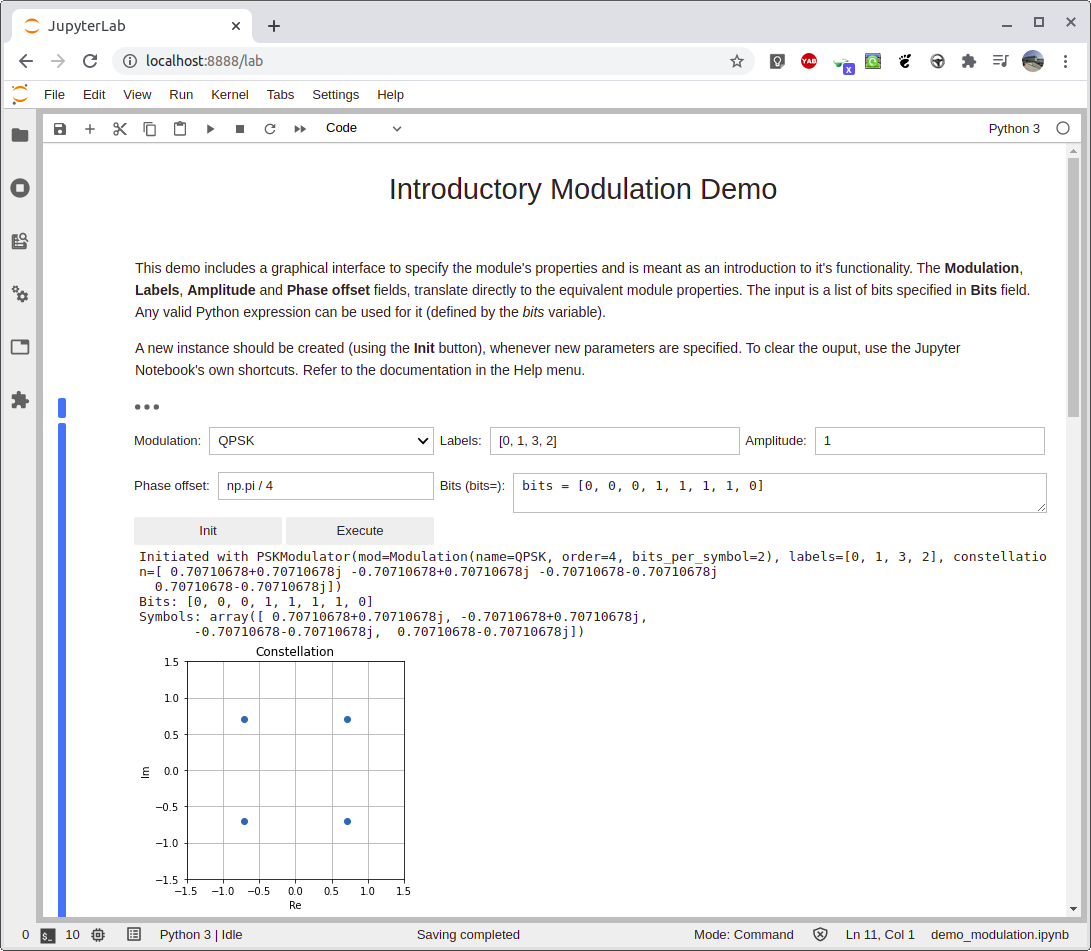
\includegraphics[width=0.75\textwidth]{demo_modulation}
  \caption{\code{PSKModulator} Jupyter notebook simple demonstration}
  \label{fig:demo_modulation}
\end{figure}

\begin{figure}[H]
  \centering
  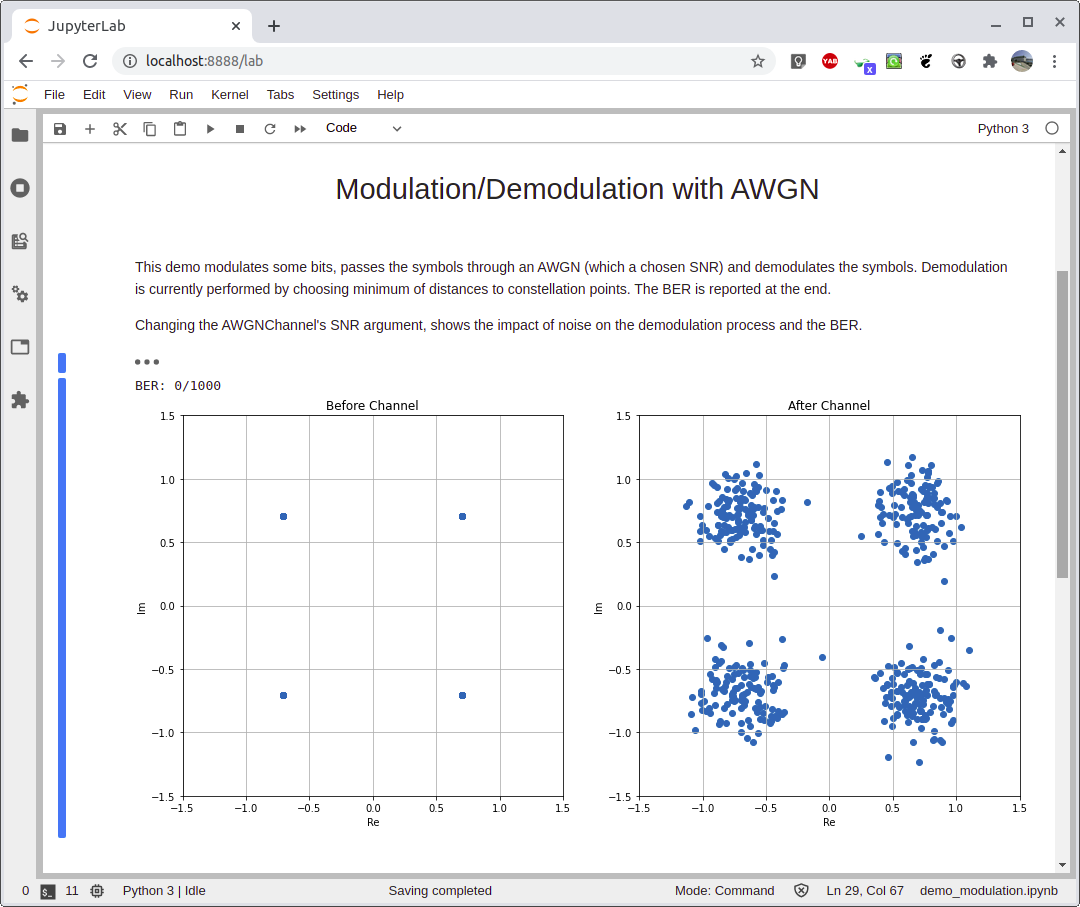
\includegraphics[width=0.75\textwidth]{demo_modulation2}
  \caption{\code{PSKModulator} Jupyter notebook demonstration with AWGN channel}
  \label{fig:demo_modulation2}
\end{figure}

%%%%%%%%%%%%%%%%%%%%%%%%%%%%%%%%%%%%%%%%%%%%%%%%%%%%%%%%%%%%%%%%%%%%%%%%%%%%%%%
\section{FIR Decimator/Interpolator}

To understand the decimation and interpolation processes, it's fundamental to grasp the concept of impulse-train sampling which simply means that samples of a discrete-time sequence $x(n)$ can be obtained by multiplying $x(n)$ by the sum of discrete-time impulse train positioned at the sampling instants $kN$, given by
\begin{align}
  p(n)=\sum_{k=-\infty}^{\infty}\delta(n-kN)
\end{align}
with DTFT
\begin{align}
  P(e^{j\Omega})=\frac{2\pi}{N}\sum_{k=-\infty}^{\infty}\delta\left(\Omega-k\frac{2\pi}{N}\right)
\end{align}

The desired sampled sequence is then:
\begin{align} \label{eq:x_pn}
  x_p(n) = x(n)p(n)
\end{align}
which is related to $x(n)$ by
\begin{align} \label{eq:x_p}
  x_p(n) =
  \begin{cases}
    x(n), & n=\text{integer} \times N\\
    0,    & \text{otherwise}\\
  \end{cases}
\end{align}

The DTFT of $x_p(n)$ can be obtained using frequency domain convolution and the sifting property for impulses:
\begin{align}
  X_p\left(e^{j\Omega}\right) &= \frac{1}{2\pi}\int_{-\pi}^{\pi}P\left(e^{j\theta}\right)X\left(e^{j\left(\Omega-\theta\right)}\right)d\theta \nonumber\\
                              &= \frac{1}{N}\sum_{k=0}^{N-1}X\left(e^{j\left(\Omega-k\frac{2\pi}{N}\right)}\right) \label{eq:X_p}
\end{align}

This result shows that sampling x$(n)$ by taking every $N$-th sample produces N copies of $X\left(e^{j\Omega}\right)$ evenly spaced in the interval $-\pi\leq\Omega\leq\pi$, with the amplitude of each copy scaled by $1/N$.

%%%%%%%%%%%%%%%%%%%%%%%%%%%%%%%%%%%%%%%
\subsection{Decimation}

The \code{FirDecimator} module filters and downsamples the input signal.

\noindent Module properties:
\begin{itemize}
  \item \code{factor}: Decimation factor
  \item \code{coeffs}: Filter coefficients
\end{itemize}

Downsampling the sequence $x(n)$ by $N$ is the process of decreasing the sampling rate by $N$ (where $N$ is specified using the \code{factor} property) by retaining the $N$-th sample of $x(n)$ to produce a new sequence $x_D(m)$. The $h_d(k)$ filter is needed to avoid aliasing, and its coefficients are provided in property \code{coeffs}. The process is illustrated in \autoref{fig:decimator}.

\begin{figure}[ht]
  \centering
  \includegraphics[width=0.75\textwidth]{decimator}
  \caption{Decimation by a factor $N$}
  \label{fig:decimator}
\end{figure}

The two sequences are related by
\begin{equation}
  x_D(m)=x(mN)
\end{equation}

Because only the $N$-th sample of $x(n)$ is of interest, $x_p(n)$, as given by \eqref{eq:x_pn}, could also be downsampled (at the proper starting point) to obtain the same sequence $x_D(m)$. The DTFT of $x_D(m)$ is then obtained as follows:
\begin{equation}
  X_D(e^{j\Omega}) = \sum_{m=-\infty}^{\infty} x_d(m)e^{-j\Omega m} = \sum_{m=-\infty}^{\infty} x_p(mN)e^{-j\Omega m}
\end{equation}

Substituting $m=n/N$, the summation can be re-expressed as
\begin{align}
  X_D(e^{j\Omega}) &= \sum_{n=\text{integer}\times N} x_p(n)e^{-j\Omega n/N} = \sum_{n=-\infty}^{\infty} x_p(n)e^{-j\Omega n/N} \nonumber\\
                   &= X_p(e^{j\Omega / N}) = \frac{1}{N} \sum_{k=0}^{N-1}X\left(e^j\left(\frac{\Omega-k2\pi}{N}\right)\right) \label{eq:X_D}
\end{align}

The relationship \eqref{eq:X_D} defines the following procedure to produce $X_D(e^{j\Omega})$ from $X(e^{j\Omega})$:
\begin{enumerate}
  \item Draw $N$ copies of $X(e^{j\Omega})$, each shifted by $2\pi k/N$ for $k=0,1,\ldots,N-1$
  \item Add the shifted copies together and scale the amplitude by $1/N$
  \item Stretch the frequency axis by $N$ by multiplying each of the `tick marks' on the frequency axis by $N$
\end{enumerate}

%%%%%%%%%%%%%%%%%%%%%%%%%%%%%%%%%%%%%%%
\subsection{Interpolation}

The \code{FirInterpolator} module upsamples and filters the input signal.

\noindent Module properties:
\begin{itemize}
  \item \code{factor}: Interpolation factor
  \item \code{coeffs}: Filter coefficients
\end{itemize}

Upsampling a sequence $x(n)$ by $N$ (where $N$ is specified using the \code{factor} property) is the process of increasing the sample rate by $N$ by inserting $N-1$ zeros between each sample of $x(n)$ to produce a new sequence $x_U(m)$. The filter $h_u(k)$ is needed for signal re-construction from the new samples, and its coefficients are provided in property \code{coeffs}. This process is illustrated in \autoref{fig:interpolator}.

\begin{figure}[ht]
  \centering
  \includegraphics[width=0.75\textwidth]{interpolator}
  \caption{Interpolation by a factor $N$}
  \label{fig:interpolator}
\end{figure}

The mathematical relationship between $x(n)$ and $x_U(m)$ is given by
\begin{equation}
x_U(m)=
  \begin{cases}
    x\left(\frac{m}{N}\right), & \text{$m=$ integer $\times$ $N$}\\
    0, & \text{otherwise}\\
  \end{cases}
\end{equation}

$X_U(m)$ looks like $x_p(m)$ from \eqref{eq:x_p}. In other words, if $x(n)$ is thought as the downsampled version of a fictitious high-rate $xx(m)$, then $x_U(m)$ can be viewed as the product $xx_p(m)=xx(m)p(m)$. Applying the relationship \eqref{eq:X_p} to $xx_p(m)$, it can be shown that the DTFT of the upsampled signal $x_U(m)$ is
\begin{equation}
X_U(e^{j\Omega})=XX_p(e^{j\Omega})=\frac{1}{N}\sum_{k-0}^{N-1} XX\left(e^{j\left(\Omega-k\frac{2\pi}{N}\right)}\right)
\end{equation}

Applying the downsampling results from \eqref{eq:X_D} , establishes the relationship between the DTFTs of and $xx(m)$ and $x(n)$:
\begin{equation}
X(e^{j\Omega})=\frac{1}{N}\sum_{k-0}^{N-1} XX\left(e^{j\left(\frac{\Omega-k2\pi}{N}\right)}\right)\implies X(e^{j\Omega N})=\frac{1}{N}\sum_{k-0}^{N-1} XX\left(e^{j\left(\Omega-k\frac{2\pi}{N}\right)}\right)
\end{equation}

Putting these results together gives the desired relationship:
\begin{equation}
X_U(e^{j\Omega})=X(e^{j\Omega N})
\end{equation}

This relationship defines the following procedure to produce $X_U(e^{j\Omega})$ from $X(e^{j\Omega})$:
\begin{enumerate}
  \item Starting with $X(e^{j\Omega})$, compress the frequency axis by $N$ by dividing all the `tick marks' on the frequency axis by $N$
  \item Draw $N-1$ shifted copies of the compressed spectrum. Each copy is shifted by $2\pi k/N$, for $k=0,1,\ldots,N-1$
\end{enumerate}

In other words, the result shows that $N$ copies of the compressed spectrum of $x(n)$ alias into the first Nyquist zone.

\autoref{fig:demo_interpolator} and \autoref{fig:demo_interpolator2} show a Jupyter notebook interface and execution for a demonstration of the \code{FirInterpolator} module. Note that the output signal (the orange trace) has a delay corresponding to 20 samples, which is $(L-1)/2$ where $L$ is the length of the interpolation filter (41 in the example shown). The filter is a \emph{square-root raised cosine} (RRC) filter with a span of 10 symbols, 4 samples per symbol, and roll off factor of 0.5.

\begin{figure}[H]
  \centering
  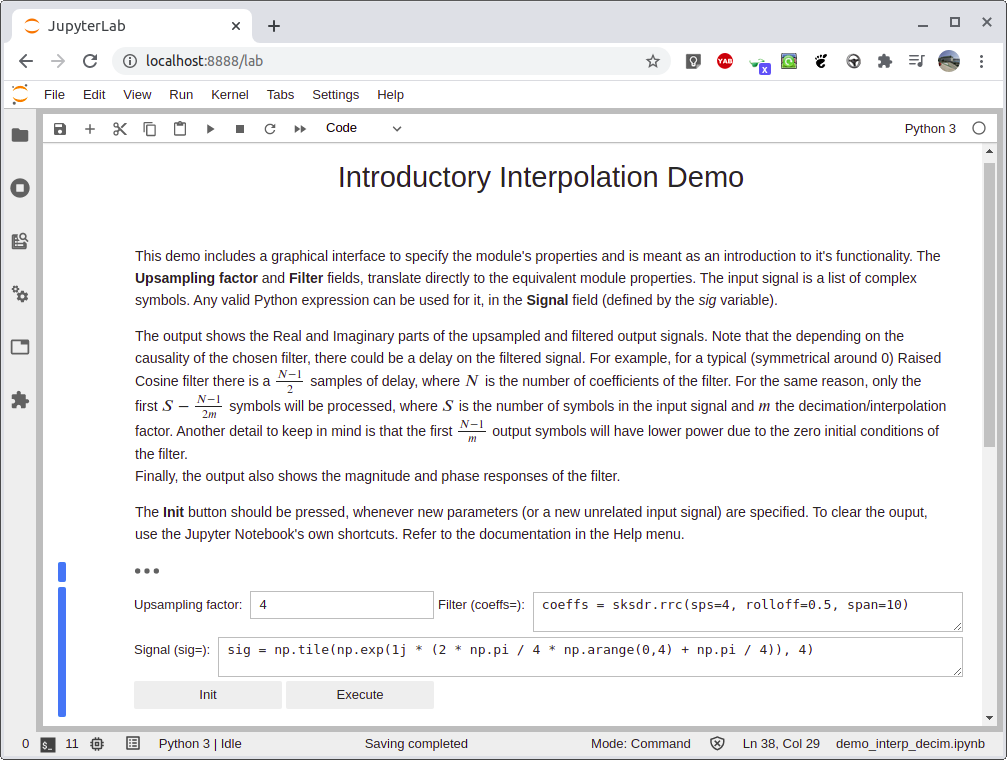
\includegraphics[width=0.75\textwidth]{demo_interpolator}
  \caption{\code{FirInterpolator} Jupyter notebook demonstration interface}
  \label{fig:demo_interpolator}
\end{figure}

\begin{figure}[H]
  \centering
  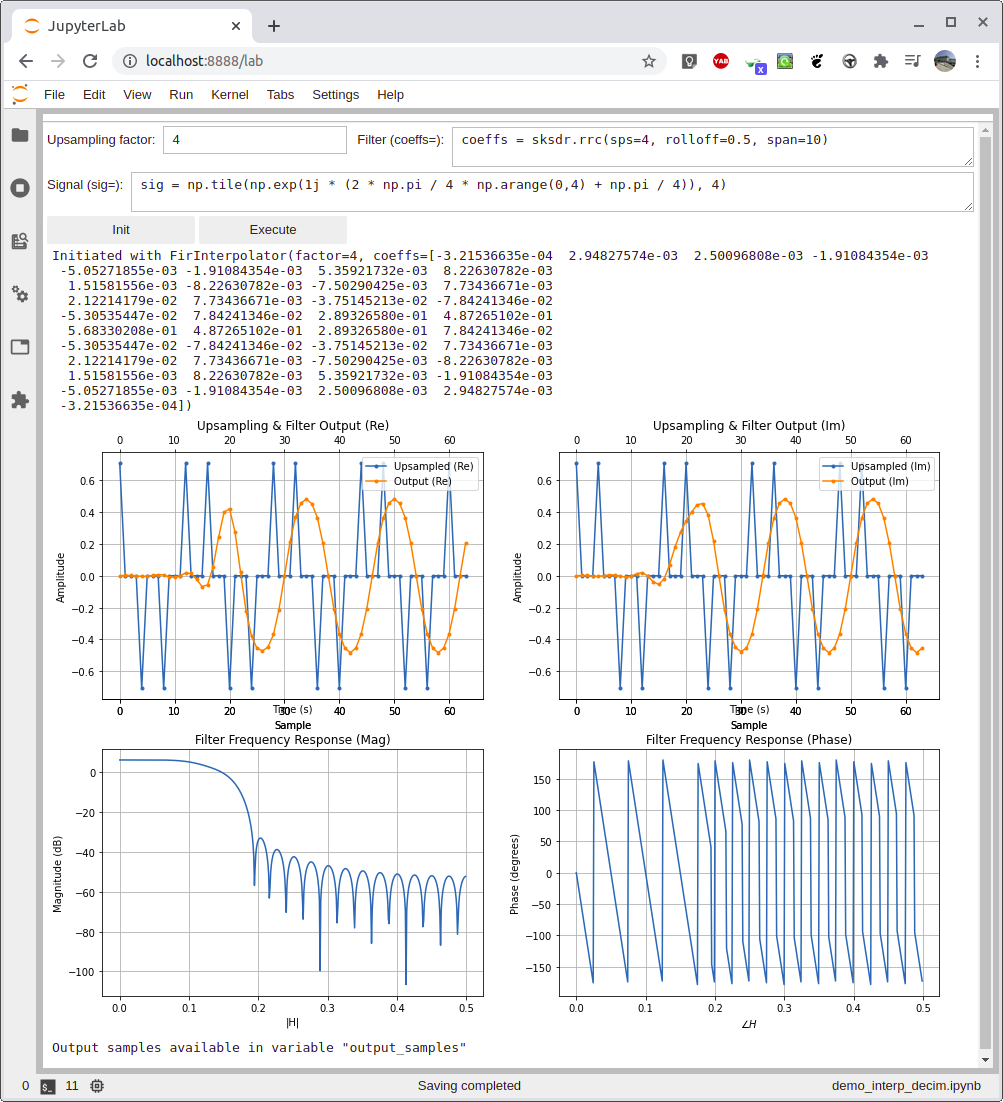
\includegraphics[width=0.75\textwidth]{demo_interpolator2}
  \caption{\code{FirInterpolator} Jupyter notebook demonstration results}
  \label{fig:demo_interpolator2}
\end{figure}

%%%%%%%%%%%%%%%%%%%%%%%%%%%%%%%%%%%%%%%%%%%%%%%%%%%%%%%%%%%%%%%%%%%%%%%%%%%%%%%
\section{Coarse Frequency Compensator}

The \code{CoarseFrequencyComp} module performs an open loop frequency correction to a PSK input signal.

\noindent Module properties:
\begin{itemize}
  \item \code{mod\_order}: Modulation order (e.g., 2 for BPSK, 4 for QPSK)
  \item \code{sample\_rate} (Hz): Input signal sampling rate
  \item \code{freq\_res} (Hz): Desired frequency resolution
\end{itemize}

The algorithm estimates the frequency error $\Delta\hat{f}$ by using a periodogram of the $m^{th}$ power of the received signal (the $m^{th}$ power is used since it removes the $m^{th}$ order PSK modulation, leaving only the carrier at a frequency $m$ times its original frequency):
\begin{equation}
\Delta\hat{f}=\frac{f_s}{m\cdot N}\underset{f}{\operatorname{argmax}}\left|\sum_{n=0}^{N-1} r(n)^m e^{-j\frac{2\pi k}{N}n}\right|
\end{equation}
where $f_s$ is the sampling frequency (specified by \code{sample\_rate}), $m$ is the modulation order (specified by \code{mod\_order}), $r(n)$ is the received sequence, and $N$ is the number of samples of the periodogram. To avoid aliasing $\Delta\hat{f}$ must be restricted to $\left[\frac{-R_{sym}}{2}, \frac{R_{sym}}{2}\right]$, where $R_{sym}=\frac{R_b}{log_2(m)}$, with $R_b$ representing the bit rate.

The algorithm effectively searches for a frequency that maximizes the time average of the $m^{th}$ power of the received signal multiplied by frequencies in the range of $\left[\frac{-R_{sym}}{2}, \frac{R_{sym}}{2}\right]$. As the form of the algorithm is the definition of the DFT of $r^{m}(n)$, searching for a frequency that maximizes the time average is equivalent to searching for a peak line in the spectrum of $r^{m}(n)$. The number of points required by the FFT is
\begin{equation}
  N=2^{log_2\left(\frac{f_s}{f_r}\right)}
\end{equation}
where $f_r$ is the desired frequency resolution, specified by \code{freq\_res}. Note that $log_2\left(\frac{f_s}{f_r}\right)$ should be rounded up, since it might not be integer.

\autoref{fig:demo_cfc} shows a Jupyter notebook with a demonstration of the \code{CoarseFrequencyComp} module. One can observe that the output signal's spectrum has been shifted, in order to correct the introduced frequency offset.

\begin{figure}[H]
  \centering
  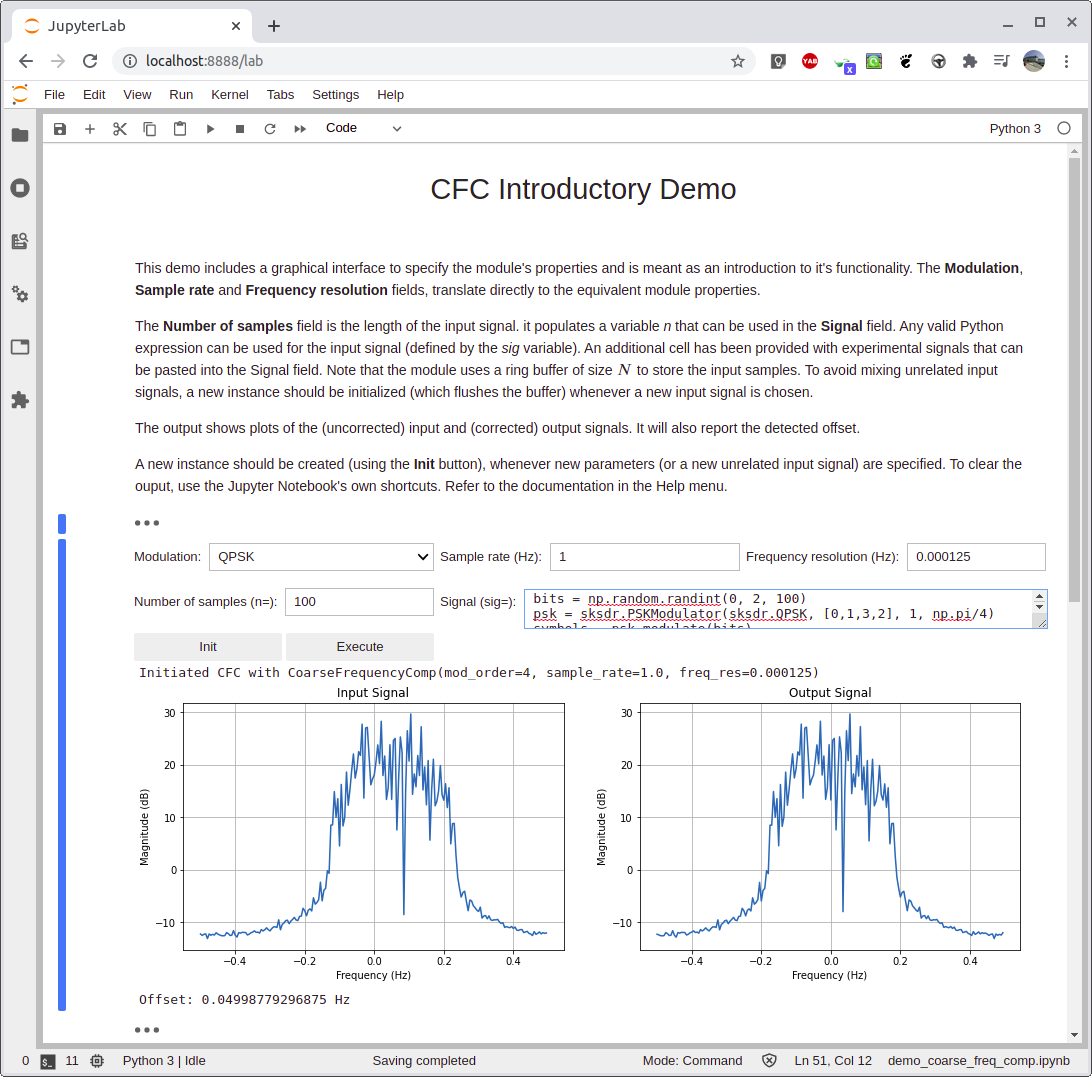
\includegraphics[width=0.75\textwidth]{demo_cfc}
  \caption{\code{CoarseFrequencyComp} Jupyter notebook demonstration}
  \label{fig:demo_cfc}
\end{figure}

%%%%%%%%%%%%%%%%%%%%%%%%%%%%%%%%%%%%%%%%%%%%%%%%%%%%%%%%%%%%%%%%%%%%%%%%%%%%%%%
\section{Carrier Frequency Synchronizer (with an introduction to PLLs)}
\label{sect:library_freq_sync}

The \code{FrequencySync} module compensates for carrier frequency and phase offsets in signals that use single-carrier modulation schemes. Currently it supports BPSK and QPSK.

\noindent Module properties:
\begin{itemize}
  \item \code{sps}: Samples per symbol of the input signal
  \item \code{mod}: Modulation of the input signal
  \item \code{damp\_factor}: PLL's damping factor
  \item \code{norm\_loop\_bw}: PLL's normalized loop bandwidth
\end{itemize}

\subsection{Phase-locked Loop Introduction}
\label{sect:pll_intro}
The module is a closed loop synchronizer that uses the discrete phase-locked loop (PLL) based algorithm described in \cite{digcomm_discrete_approach}. PLLs are often used in digital communications to synchronize local oscillators in the receiver to oscillators used in the transmitter (carrier phase synchronization) or to synchronize the data clock in the receiver to the transmitter data clock (symbol timing synchronization). In either case, the PLL can be though as a device that tracks the phase and frequency of a sinusoid. A basic structure of a PLL is shown in \autoref{fig:analog_pll}.

\begin{figure}[ht]
  \centering
  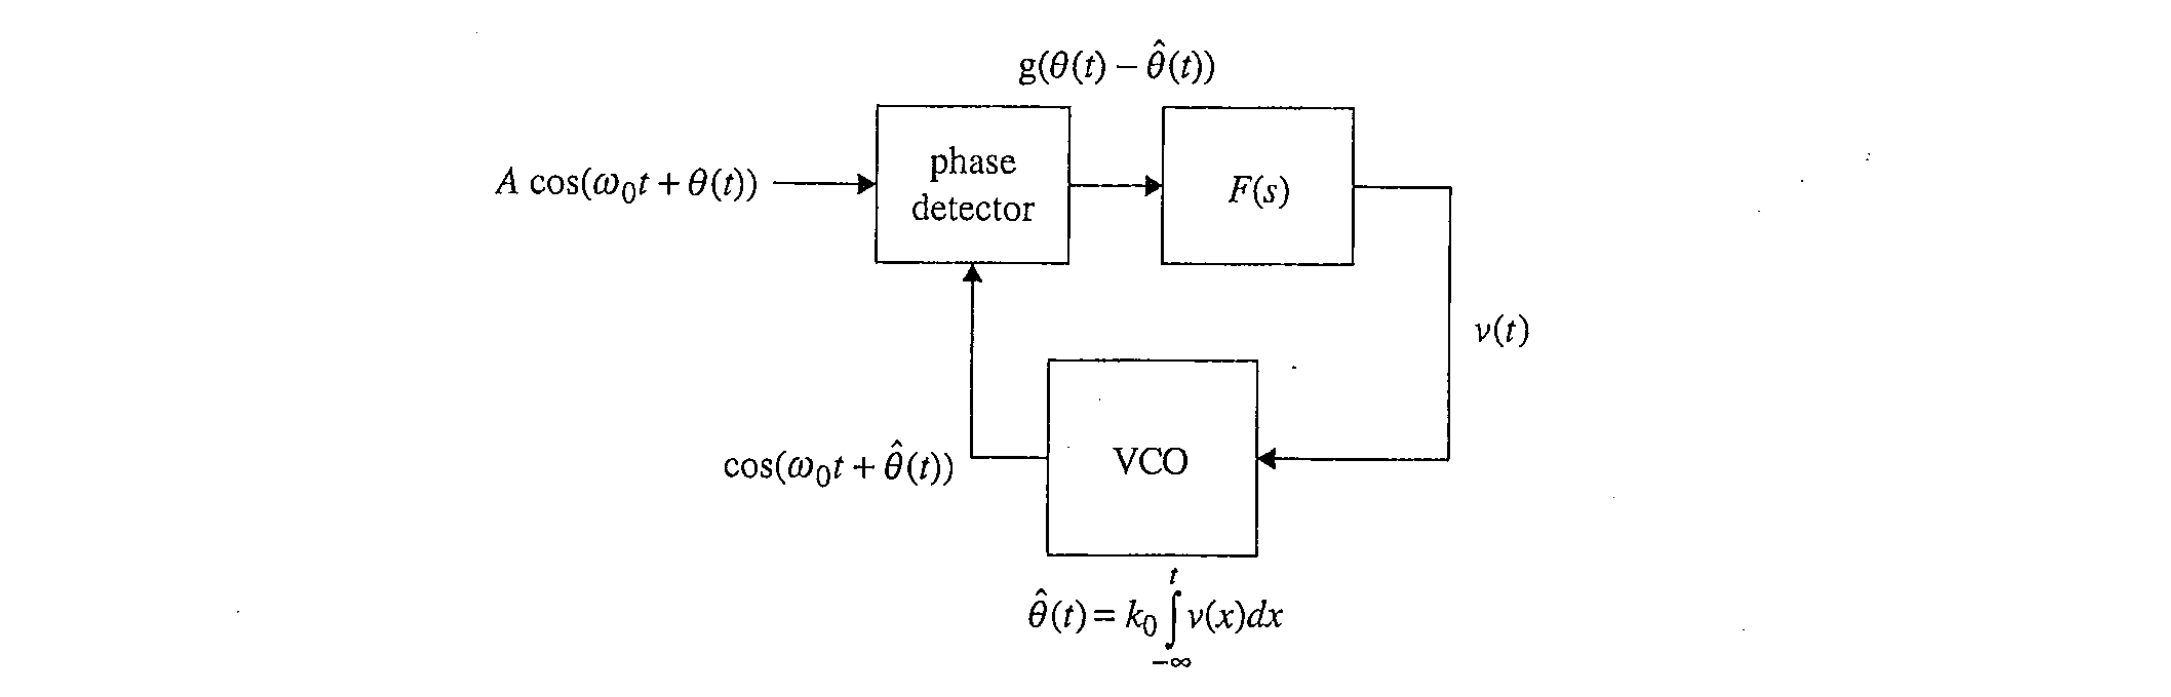
\includegraphics[width=\textwidth]{analog_pll}
  \caption{Basic structure of phase locked loop [\citeauthor{digcomm_discrete_approach}]}
  \label{fig:analog_pll}
\end{figure}

It's also common to produce a \emph{phase equivalent} representation writing down the phases of all sinusoids and tracking the operations on those phases through the PLL. This structure is illustrated in \autoref{fig:analog_pll_phases}.

\begin{figure}[ht]
  \centering
  
\includegraphics[width=\textwidth]{analog_pll_phases}
  \caption{Phase equivalent PLL corresponding to the PLL in \autoref{fig:analog_pll} [\citeauthor{digcomm_discrete_approach}]}
  \label{fig:analog_pll_phases}
\end{figure}

The system is composed of three blocks: the phase detector, the loop filter and the voltage-controlled oscillator (VCO). The loop input $\theta(t)$ and the VCO output $\hat\theta(t)$ are the inputs to the phase detector, and the difference in phase between these inputs is known as the \emph{phase error} $\theta_e(t)=\theta(t) -\hat\theta(t)$. The output of the phase detector is a function of this phase error $g(\theta_e)$. This, in turn, is filtered by the loop filter to produce an input to the VCO which controls its output phase. When functioning correctly, the loop adjusts the control voltage $v(t)$ to produce a phase estimate $\hat\theta(t)$ that drives the phase error to zero. \autoref{fig:s-curve} shows the plot of the phase detector output $g(\theta_e(t)$. When the phase error is positive, $\theta(t) > \hat \theta(t)$, which means the phase of the VCO output lags the loop input and must be increased. The phase error produces a control input voltage $v(t)$ on the VCO, which in turn increases its output phase, producing the desired results. When the phase error is negative, $\theta(t) < \hat \theta(t)$, a negative control voltage is produced and the VCO decreases its output phase.

\begin{figure}[ht]
  \centering
  
\includegraphics[width=\textwidth]{s-curve}
  \caption{Typical phase detector input-output curve known as an `S curve' [\citeauthor{digcomm_discrete_approach}]}
  \label{fig:s-curve}
\end{figure}

To derive the system parameters we can start with an analogue PLL structure and then obtain the equivalent parameters in the digital domain.

Given that the phase detector can be a non-linear function, a common method of analysing these systems is to linearize them around a desired operation point (in this case $\theta_e=0$). The linear approximation is obtained by considering that $g(\theta_e)\approx k_p \theta_e$, for small $\theta_e$. Having a linear system, the phase equivalent diagram can now be analysed using frequency domain techniques (Laplace or Z transforms) to extract the parameters that characterize the properties and performance of the system. \autoref{fig:analog_pll_linear} shows the linearized system in the time and frequency domains.

\begin{figure}[ht]
  \centering
  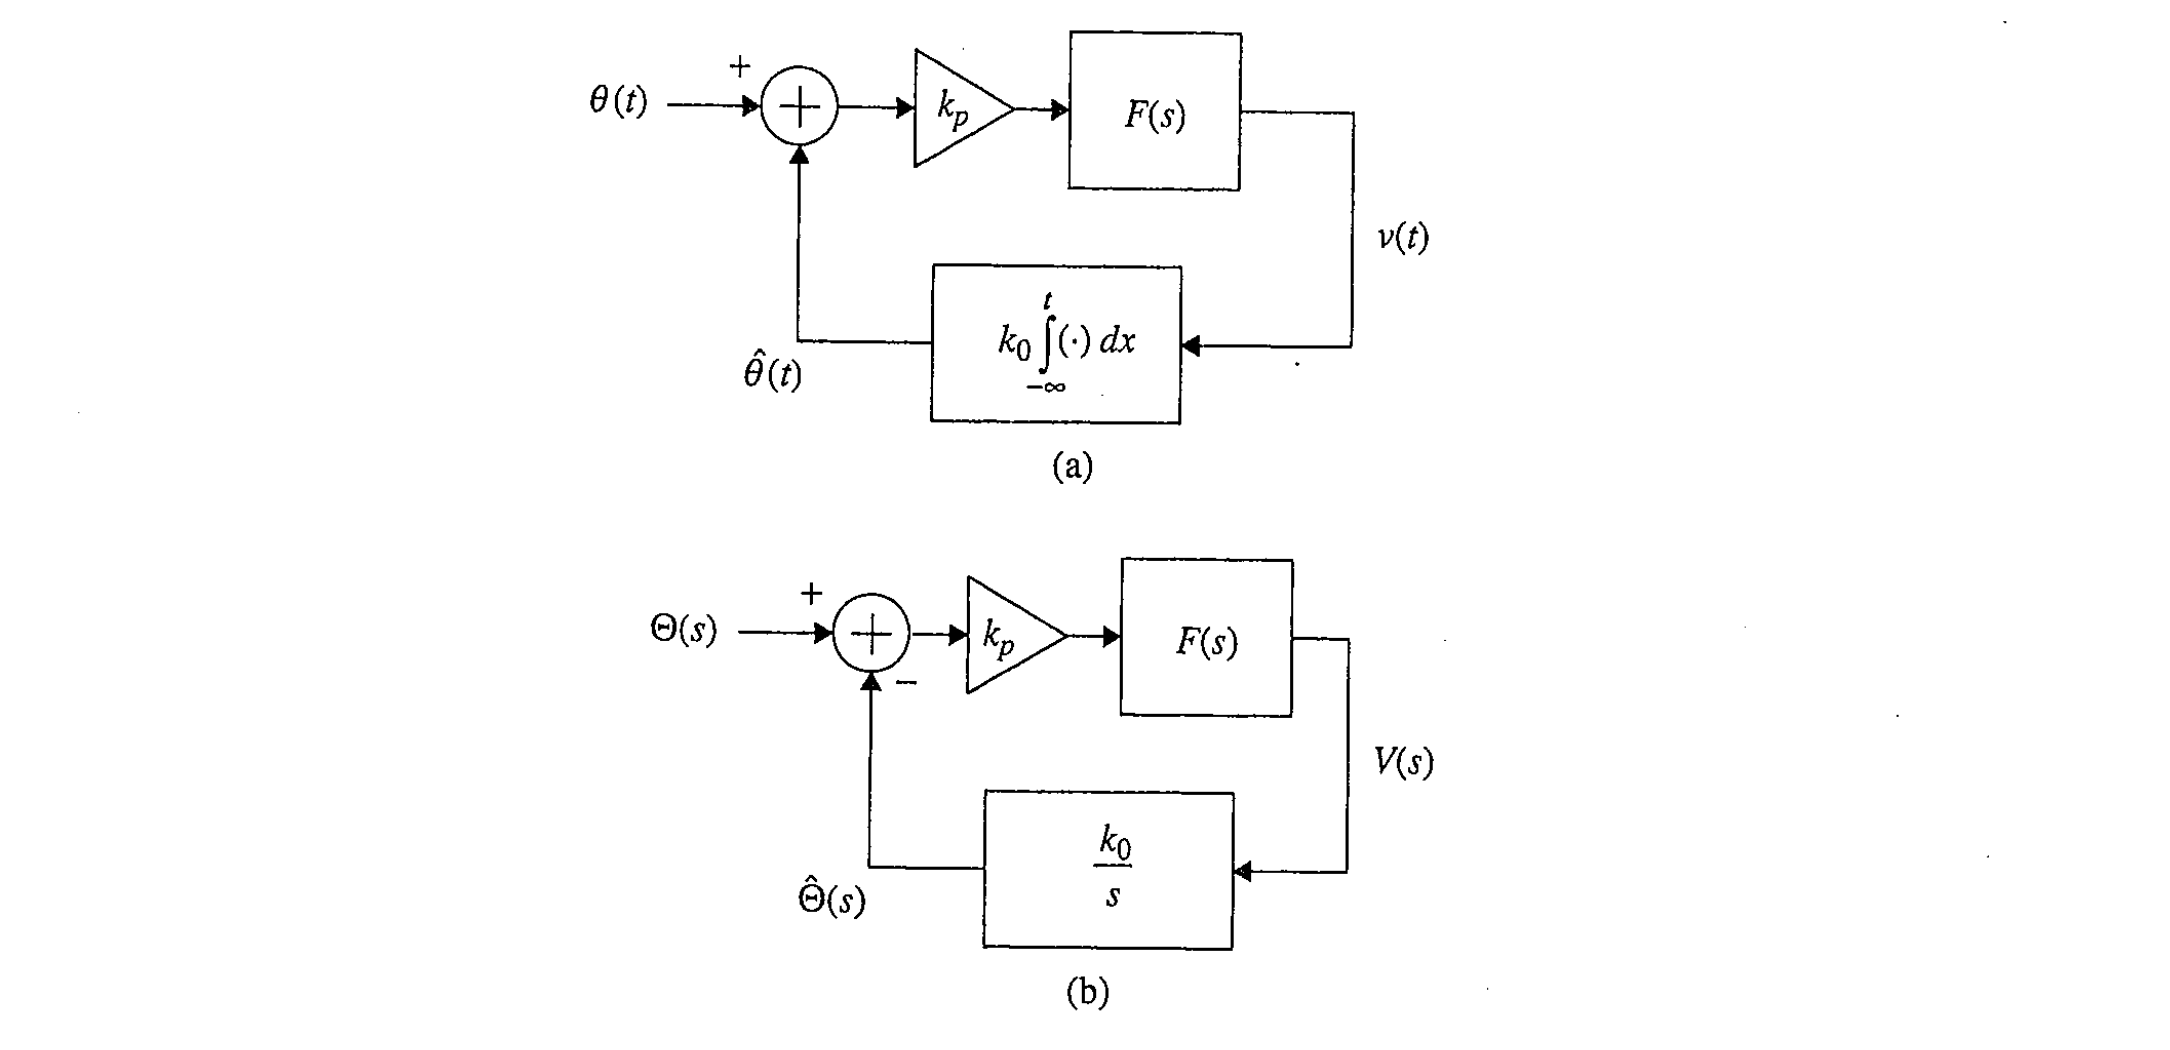
\includegraphics[width=\textwidth]{analog_pll_linear}
  \caption{Linearized equivalent, both in time and frequency domains, of the PLL show in \autoref{fig:analog_pll} [\citeauthor{digcomm_discrete_approach}]}
  \label{fig:analog_pll_linear}
\end{figure}

Two particular input signals (the phase step input (corresponding to a constant phase offset: $\theta(t) = \Delta\theta\cdot u(t)$) and the phase ramp input (corresponding to a constant frequency offset: $\theta(t) = (\Delta \omega)t\cdot u(t)$)) are used to analyse the \emph{phase error response}. The transfer function for the phase error detector is
\begin{equation}
  G(s)=\frac{\Theta_e(s)}{\Theta(s)}=\frac{s}{s+k_0 k_p F(s)}
\end{equation}

replacing the Laplace transforms of the step and ramp inputs (respectively $\Theta_{step}(s)=\frac{\Delta \theta}{s}$ and $\Theta_{ramp}(s)=\frac{\Delta \omega}{s^2}$) into that expression, allows obtaining the phase error responses:
\begin{align}
\Theta_{e,step}(s) & =\frac{\Delta\theta}{s+k_0 k_p F(s)}\\
\Theta_{e,ramp}(s) & =\frac{\Delta\omega}{s^2+s k_0 k_p F(s)}
\end{align}

applying the final value theorem one extracts the conditions on the loop filter:
\begin{align}
\theta_{e,step}(\infty) & =\lim_{s\to 0}\left(s\cdot\Theta_{e,step}(s)\right)=0\text{, if }F(0)\neq0\\
\theta_{e,ramp}(\infty) & =\lim_{s\to 0}\left(s\cdot\Theta_{e,ramp}(s)\right)=0\text{, if }F(0)=\infty
\end{align}

It can be seen that to force the phase error $\theta_e$ to 0, the loop must have a non-zero DC gain (condition imposed by the step response), and an infinite DC gain (condition imposed by the ramp response). A \emph{proportional-plus-integrator} has these properties. Notice that while it's difficult to implement an infinite DC gain integrator in the analogue domain, it is straightforward in the digital domain and so this is the chosen structure for the loop filter:
\begin{equation}F(s)=k_1+\frac{k_2}{s}\end{equation}

To extract the loop performance in turn, the \emph{output response} is analysed:
\begin{equation}H_a(s)=\frac{\hat\Theta(s)}{\Theta(s)}=\frac{k_0 k_p F(s)}{s+k_0 k_p F(s)}\end{equation}

With $F(s)$ as a proportional-plus-integrator loop filter, this becomes
\begin{equation}H_a(s)=\frac{\hat\Theta(s)}{\Theta(s)}=\frac{k_0 k_p k_1 s + k_0 k_p k_2}{s^2+k_0 k_p k_1 s + k_0 k_p k_2}\end{equation}

This is a second order system (it has two poles, one originating from the loop filter and the other from the VCO) and so it can be expressed in the familiar form
\begin{equation} \label{eq:Ha_s}
  H_a(s)=\frac{2\zeta \omega_n s+\omega_n^2}{s^2+2\zeta \omega_n s+\omega_n^2}
\end{equation}
where
\begin{align}
\zeta & =\frac{k_1}{2}\sqrt{\frac{k_0 k_p}{k_2}}\\
\omega_n & = \sqrt{k_0 k_p k_2}
\end{align}
are the \emph{damping factor} and \emph{natural frequency} of the system.

Sometimes it's common to specify the 3-dB bandwidth of the PLL $\omega_{3dB}$, obtained by setting $|H_a(j\omega)|^2=\frac{1}{2}$ and solving for $\omega$. In this case
\begin{equation}\omega_{3dB}=\omega_n \sqrt{1+2\zeta^2+\sqrt{(1+2\zeta^2)^2+1}}\end{equation}

While this maybe a familiar concept, $\omega_{3dB}$ is not very useful as a measure of the bandwidth of a PLL, so an alternative parameter is $B_n$, the \emph{equivalent noise bandwidth}, defined as the bandwidth of a fictitious rectangular low-pass filter with the same area as $|H_a(j\omega)|^2$. With a proportional-plus-integrator filter, this turns out to be
\begin{equation}B_n=\frac{\omega_n}{2}\left(\zeta+\frac{1}{4\zeta}\right)\end{equation}

With equations for $\zeta$, $\omega_n$ and $B_n$, it's possible, in turn, to obtain expressions for the loop constants:
\begin{align}
k_p k_0 k_1 &= \frac{4\zeta B_n}{\zeta+\frac{1}{4\zeta}}\\
k_p k_0 k_2 &= \frac{4 B_n^2}{\left(\zeta+\frac{1}{4\zeta}\right)^2}
\end{align}

With this analysis, one is now in the position to derive the equivalent discrete-time PLL structure. Using the bilinear transform, it's possible obtain the corresponding discrete-time PLL parameters. \autoref{fig:discrete_pll_basic_and_phases} shows the basic structure of a discrete-time PLL and the corresponding phase equivalent PLL.

\begin{figure}[ht]
  \centering
  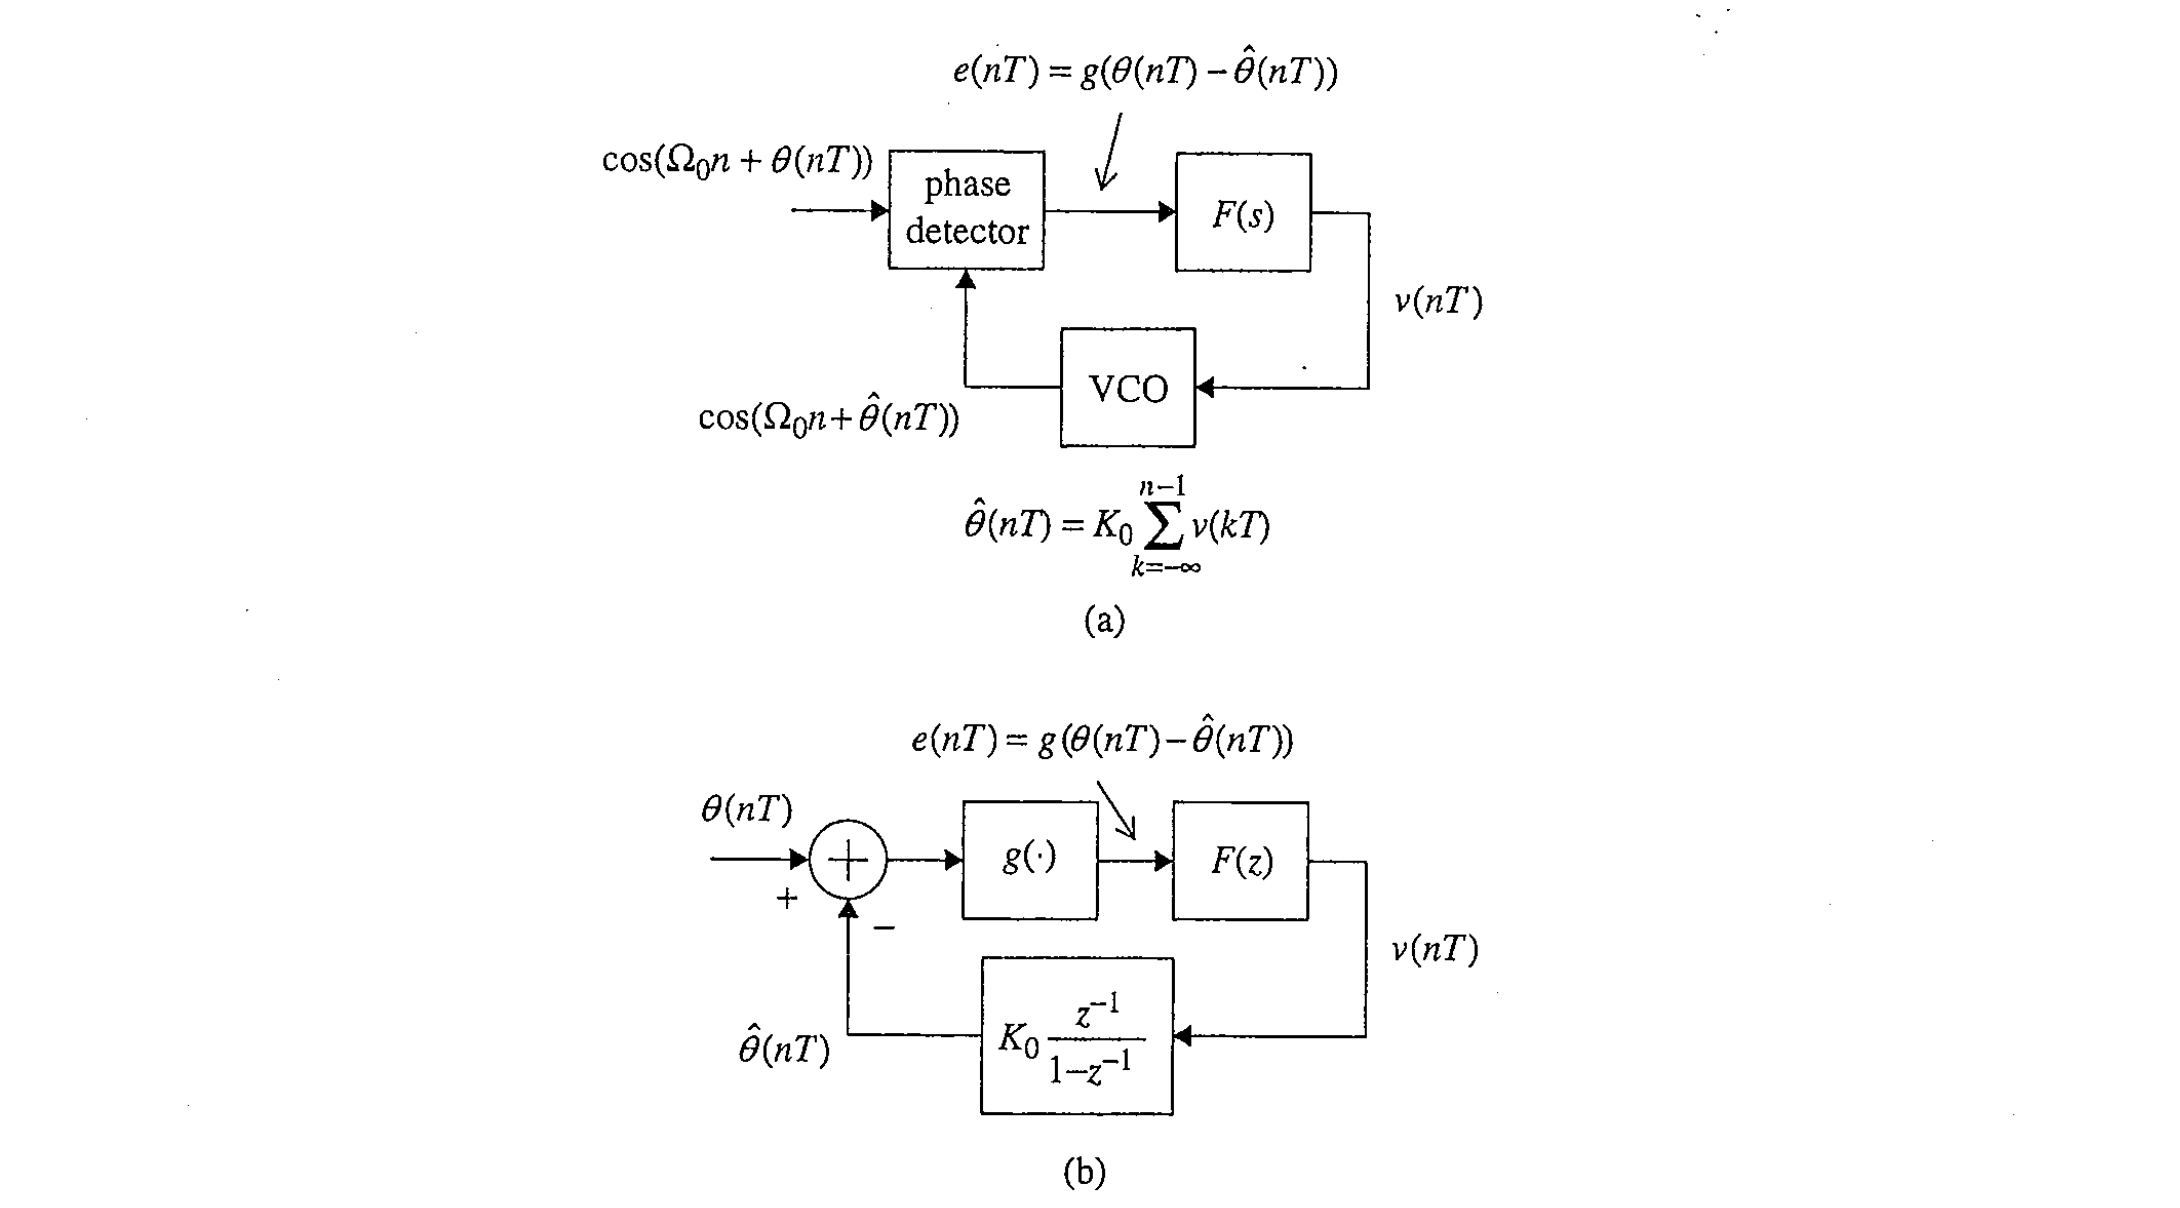
\includegraphics[width=\textwidth]{discrete_pll_basic_and_phases}
  \caption{Basic structure of a discrete-time PLL a) and the corresponding phase equivalent PLL b) [\citeauthor{digcomm_discrete_approach}]}
  \label{fig:discrete_pll_basic_and_phases}
\end{figure}

If one introduces in the general block diagram of a PLL, the assumptions made (a constant phase detector gain $k_p$ and the a proportional-plus-integrator filter), then the detailed linearized structure of both the PLL and its phase equivalent emerges, and is shown in \autoref{fig:analog_pll_pplus_int_and_linear_phase_equiv} for the continuous-time case, and in \autoref{fig:digital_pll_pplus_int_and_linear_phase_equiv} for the discrete-time case. The direct digital synthesizer (DDS) is the discrete-time equivalent of the VCO. These two figures serve as a useful reference for the following derivation of the discrete-time PLL parameters.

\begin{figure}[H]
  \centering
  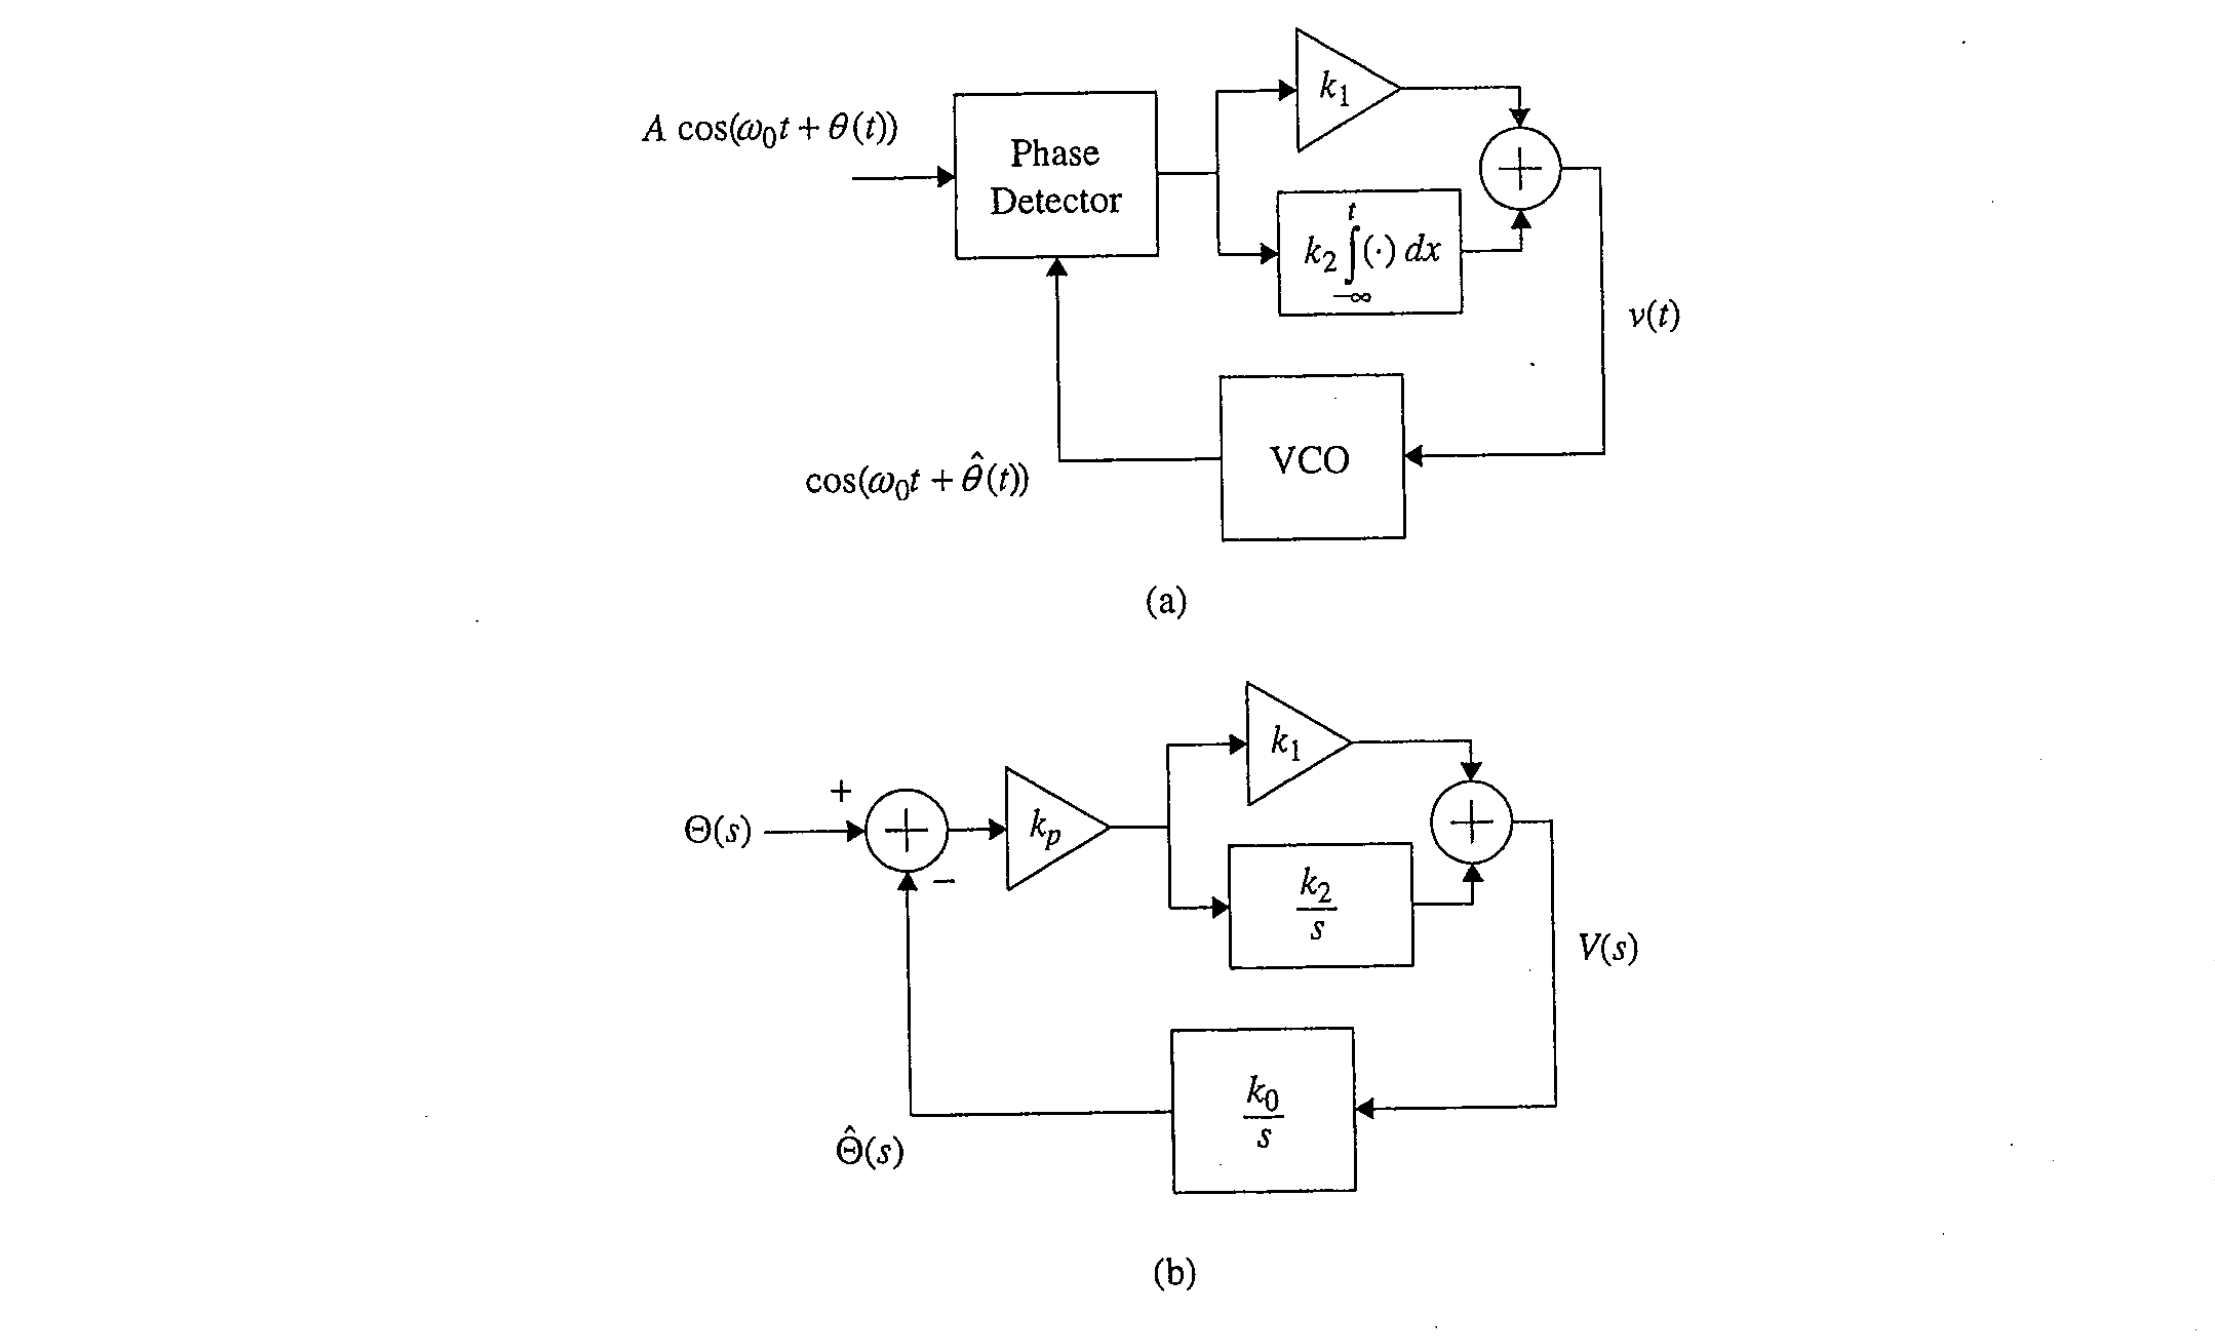
\includegraphics[width=\textwidth]{analog_pll_pplus_int_and_linear_phase_equiv}
  \caption{Second-order continuous-time phase locked loop with proportional-plus-integrator loop filter (a) and the linearized phase equivalent PLL (b) [\citeauthor{digcomm_discrete_approach}]}
  \label{fig:analog_pll_pplus_int_and_linear_phase_equiv}
\end{figure}

\begin{figure}[H]
  \centering
  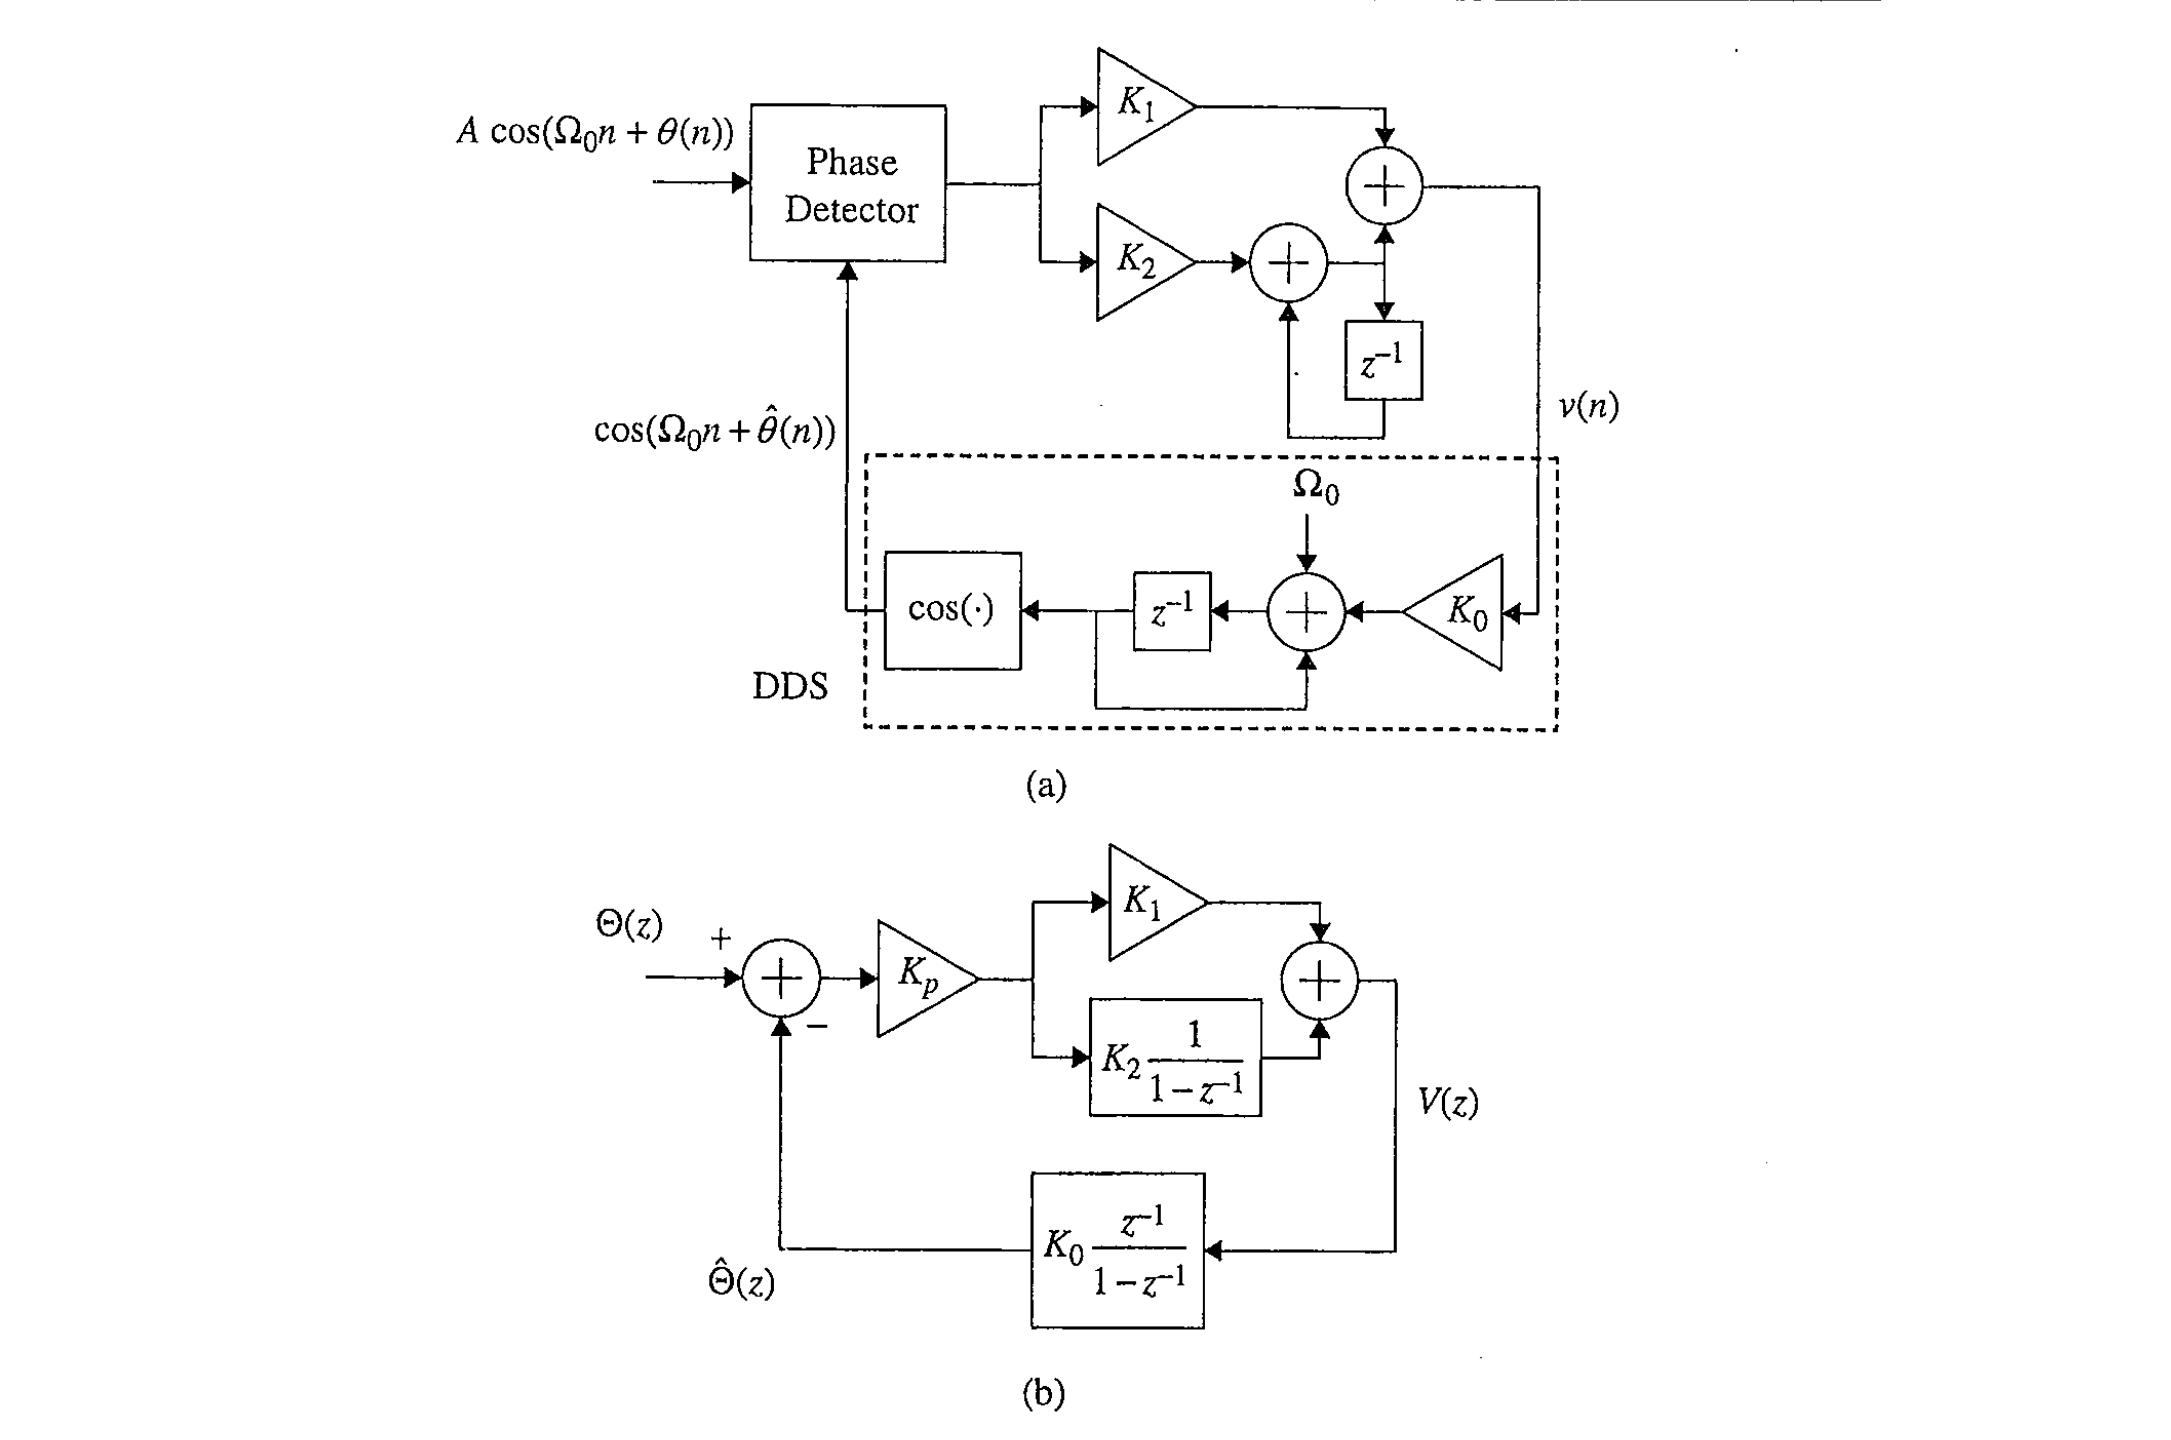
\includegraphics[width=\textwidth]{digital_pll_pplus_int_and_linear_phase_equiv}
  \caption{Second-order discrete-time phase locked loop with proportional-plus-integrator loop filter  that mimics the continuous-time PLL in \autoref{fig:analog_pll_pplus_int_and_linear_phase_equiv} (a) and the linearized phase equivalent discrete-time PLL (b) [\citeauthor{digcomm_discrete_approach}]}
  \label{fig:digital_pll_pplus_int_and_linear_phase_equiv}
\end{figure}

One already knows the continuous output response from \eqref{eq:Ha_s}. From \autoref{fig:digital_pll_pplus_int_and_linear_phase_equiv} it is possible to derive the discrete-time equivalent:
\begin{equation}H_d(z)=\frac{K_p K_0 (K_1+K_2)z^{-1}-K_p K_0 K_1 z^{-2}}{1-2\left(1-\frac{1}{2}K_p K_0 \left(K_1+K_2\right)
\right)z^{-1}+\left(1-K_p K_0 K_1 \right)z^{-2}}\end{equation}

Applying Tustin's equation (bilinear transform) to $H_a(s)$ produces $H_a\left(\frac{2}{T}\frac{1-z^{-1}}{1+z^{-1}}\right)$. Equating and rearranging the denominators of $H_a\left(\frac{2}{T}\frac{1-z^{-1}}{1+z^{-1}}\right)$ and $H_d(z)$, and solving for the loop constants finally produces
\begin{align}
K_p K_0 K_1 &= \frac{4\zeta\theta_n}{1+2\zeta\theta_n+\theta_n^2}\\
K_p K_0 K_2 &= \frac{4\theta_n^2}{1+2\zeta\theta_n+\theta_n^2}
\end{align}
where
\begin{equation}\theta_n=\frac{\omega_n T}{2}\end{equation}
which can be re-expressed in terms of $B_n$ and $\zeta$, given the relations obtained in the proportional-plus-integrator loop filter case:
\begin{equation}\theta_n=\frac{B_n T}{\zeta+\frac{1}{4\zeta}}=\frac{B_n T_s}{N\left(\zeta+\frac{1}{4\zeta}\right)}\end{equation}
where $T$ is the sampling period, $T_s$ the symbol period and $N$ the number of samples per symbol.

Replacing this in the loop constant equations gives
\begin{align}
K_p K_0 K_1 &= \frac{4\zeta\left(\frac{B_n T_s}{N\left(\zeta+\frac{1}{4\zeta}\right)}\right)}{1+2\zeta\left(\frac{B_n T_s}{N\left(\zeta+\frac{1}{4\zeta}\right)}\right)+\left(\frac{B_n T_s}{N\left(\zeta+\frac{1}{4\zeta}\right)}\right)^2}\\
K_p K_0 K_2 &= \frac{4\left(\frac{B_n T_s}{N\left(\zeta+\frac{1}{4\zeta}\right)}\right)^2}{1+2\zeta\left(\frac{B_n T_s}{N\left(\zeta+\frac{1}{4\zeta}\right)}\right)+\left(\frac{B_n T_s}{N\left(\zeta+\frac{1}{4\zeta}\right)}\right)^2}
\end{align}
which, when, as often is the case, $B_nT\ll1$, can be approximated as
\begin{align}
\label{eq:digital_loop_constants1} K_p K_0 K_1 &\approx \frac{4\zeta}{\zeta+\frac{1}{4\zeta}}\frac{B_n T_s}{N}\\
\label{eq:digital_loop_constants2} K_p K_0 K_2 &\approx \frac{4}{\left(\zeta+\frac{1}{4\zeta}\right)^2}\left(\frac{B_n T_s}{N}\right)^2
\end{align}

Note that, in this approximation, where the sample rate is large relative to the equivalent loop bandwidth, the discrete-time expressions are the same as those for the continuous-time loop case, except that the loop bandwidth is normalized by the sample rate (or the symbol rate).

\subsection{PLL design for PSK carrier frequency synchronization}
Up until this point, the structure of a general discrete-time PLL has been derived, with the exception of the phase error detector, which has been assumed only to be linear, more specifically $g(\theta_e)=K_p\theta_e$. Unfortunately this general case does not work for the specific case of PSK modulations because if this PLL was applied to the input signal it would try to track both the carrier phase error and the phase offsets introduced by the modulation itself. Thus the PLL must \emph{remove} the modulation phase shifts and track only the remaining phase. The \emph{maximum likelihood} (ML) phase error detector is chosen instead, which consists of minimizing the energy in $\theta_e$. It also has the advantage of avoiding arctangent operations required by other phase detectors based on a purely geometric approach. \autoref{fig:complete_digital_pll} shows the complete discrete-time PLL (for QPSK modulation case) with the proposed ML phase error detector.
\begin{figure}[ht]
  \centering
  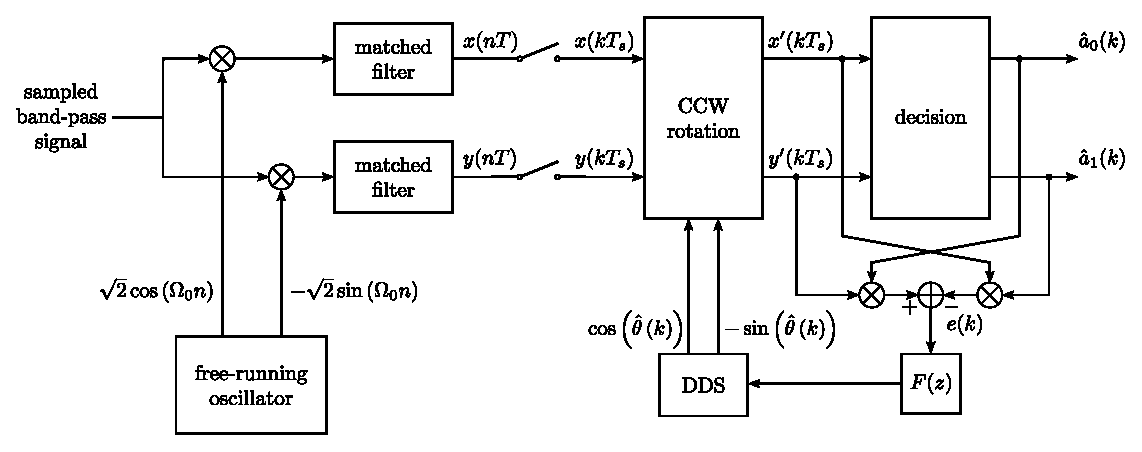
\includegraphics[width=\textwidth]{drawing}
  \caption{Block diagram for the QPSK carrier phase PLL using an error signal based on the ML phase error detector}
  \label{fig:complete_digital_pll}
\end{figure}
The ML phase detector first de-rotates the input signal by the estimated phase from the DDS output (CCW rotation block). This leaves only the phase of the received data symbol $\theta_r = \theta-\hat\theta$. It then subtracts the phase of the transmitted data symbol to obtain the phase error, $\theta_e=\theta_r-\theta_d$. This is usually used in a \emph{data-aided} system, in which there is a training sequence where the transmission symbols are well known. If the symbols are unknown then it is called a \emph{decision-directed} system and the transmitted symbols must be estimated. In that case, $\theta_e$ is more accurately denoted by $\theta_e=\theta_r-\hat\theta_d$. The latter is the situation in this case. It can be shown \cite{digcomm_discrete_approach} that the ML phase detector response is given by
\begin{align}
  e(k)=y'(kT_s)\hat a_0(k)-x(kT_s)'\hat a_1(k)
\end{align}

For QPSK the decisions are
\begin{align}
\hat a_0(k) &= A\times\operatorname{sgn}\left[x(kT_s)'\right] \\
\hat a_1(k) &= A\times\operatorname{sgn}\left[y(kT_s)'\right]
\end{align}

Expressing $x'(kT_s)$ and $y'(kT_s)$ in terms of $\theta_e$, $a_0(k)$ and $a_1(k)$, and averaging over all four possible symbols, produces the S-curve for the ML phase error detector for the data-aided case:
\begin{align}
\overline{g}_{\text{QPSK}}(\theta_e) &= 2KA^2\sin(\theta_e)\approx 2KA^2\theta_e\text{, for }\theta_e\approx0\\
\overline{g}_{\text{BPSK}}(\theta_e) &= KA^2\sin(\theta_e)\approx KA^2\theta_e\text{, for }\theta_e\approx0
\end{align}
where $K$ is the amplitude of the received signal and $A$ is the norm of symbols. This gives the desired $K_p$:
\begin{align}
K_{p_{\text{QPSK}}} &= 2KA^2\\
K_{p_{\text{BPSK}}} &= KA^2
\end{align}

The decision-directed case, is given by
\begin{align}
  \overline{g}_{\text{QPSK}}(\theta_e)=
    \begin{cases}
      -2KA^2 \sin(\theta_e), &-\pi\leq\theta_e<-\frac{3\pi}{4}\\
      2KA^2 \cos(\theta_e), &-\frac{3\pi}{4}<\theta_e<-\frac{\pi}{4}\\
      2KA^2 \sin(\theta_e), &-\frac{\pi}{4}<\theta_e<\frac{\pi}{4}\\
      -2KA^2 \cos(\theta_e), &\phantom{-}\frac{\pi}{4}<\theta_e<-\frac{3\pi}{4}\\
      -2KA^2 \sin(\theta_e), &\phantom{-}\frac{3\pi}{4}<\theta_e\leq\pi
    \end{cases}
\end{align}
and
\begin{align}
  \overline{g}_{\text{BPSK}}(\theta_e)=
    \begin{cases}
      -KA^2 \sin(\theta_e), &-\pi\leq\theta_e<-\frac{\pi}{2}\\
      KA^2 \sin(\theta_e), &-\frac{\pi}{2}<\theta_e<\frac{\pi}{2}\\
      -KA^2 \sin(\theta_e), &\phantom{-}\frac{\pi}{2}<\theta_e<\pi
    \end{cases}
\end{align}

\autoref{fig:s_curve_qpsk} and \autoref{fig:s_curve_bpsk} show the S-curves for the QPSK and BPSK data-aided and decision-directed ML phase detectors. Note, again, that for $\theta_e\approx0$, $\overline{g}_{\text{QPSK}}(\theta_e)\approx 2KA^2\theta_e$, from which $K_{p_{\text{QPSK}}} = 2KA^2$ (similarly, $K_{p_{\text{BPSK}}} = KA^2$).
\begin{figure}[ht]
  \centering
  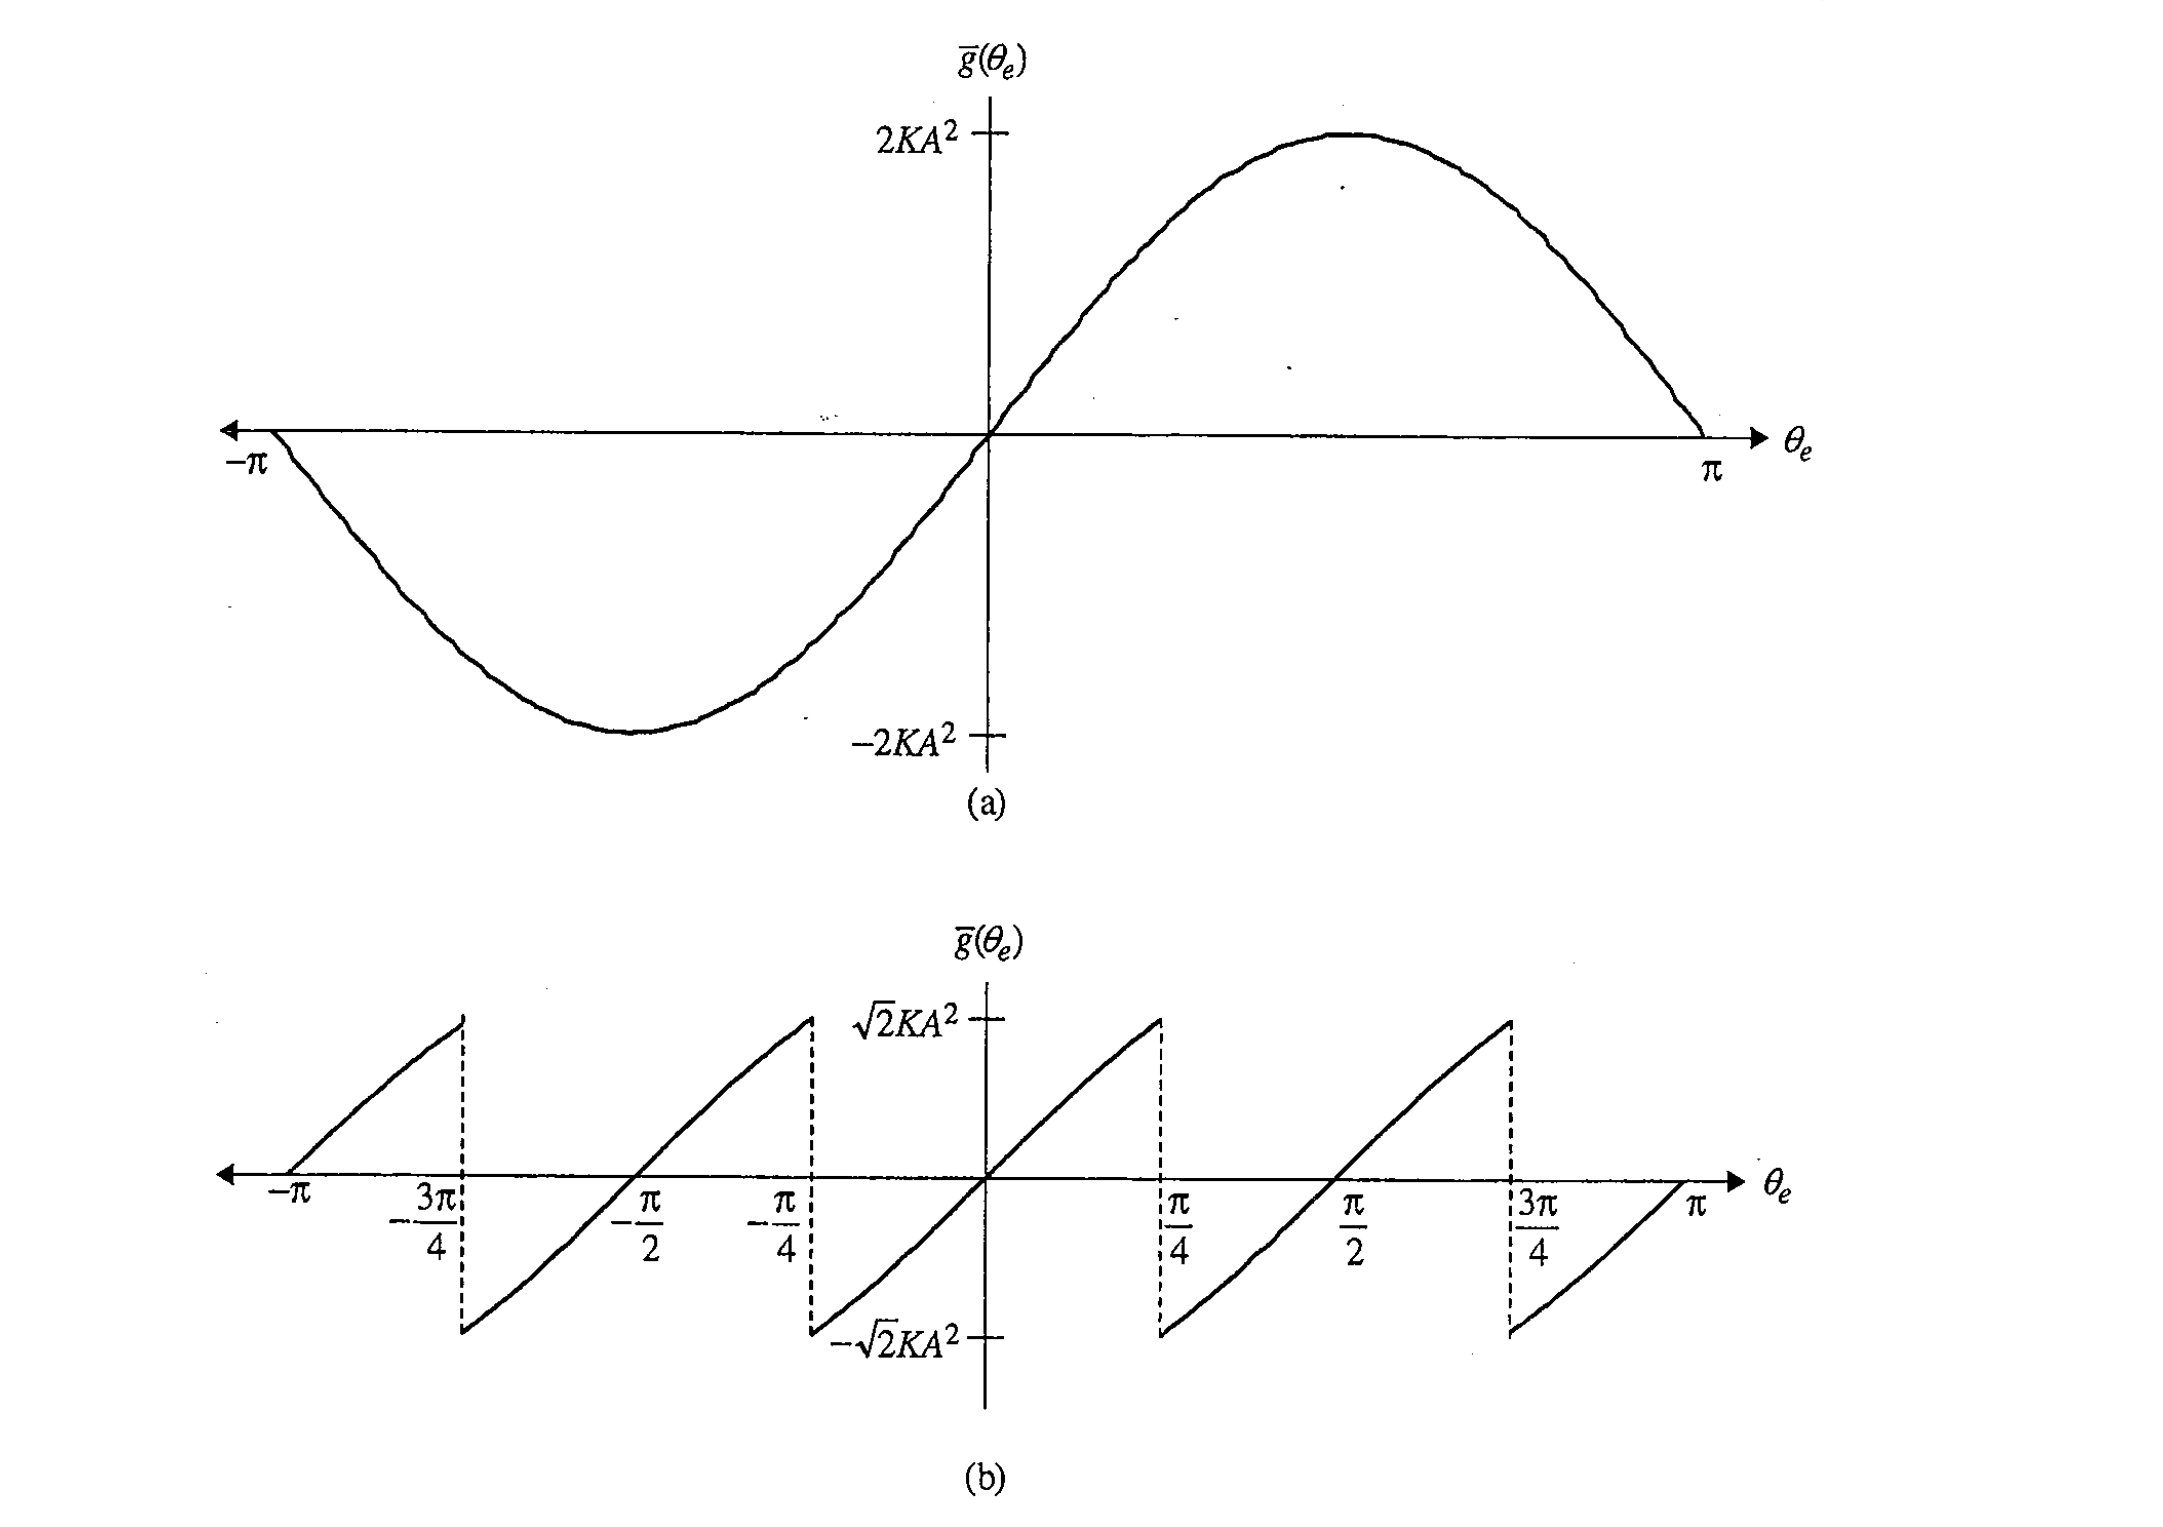
\includegraphics[width=\textwidth]{s_curve_qpsk}
  \caption{S-curves for the a) data-aided QPSK phase detector and b) the decision-directed QPSK phase detector [\citeauthor{digcomm_discrete_approach}]}
  \label{fig:s_curve_qpsk}
\end{figure}

\begin{figure}[ht]
  \centering
  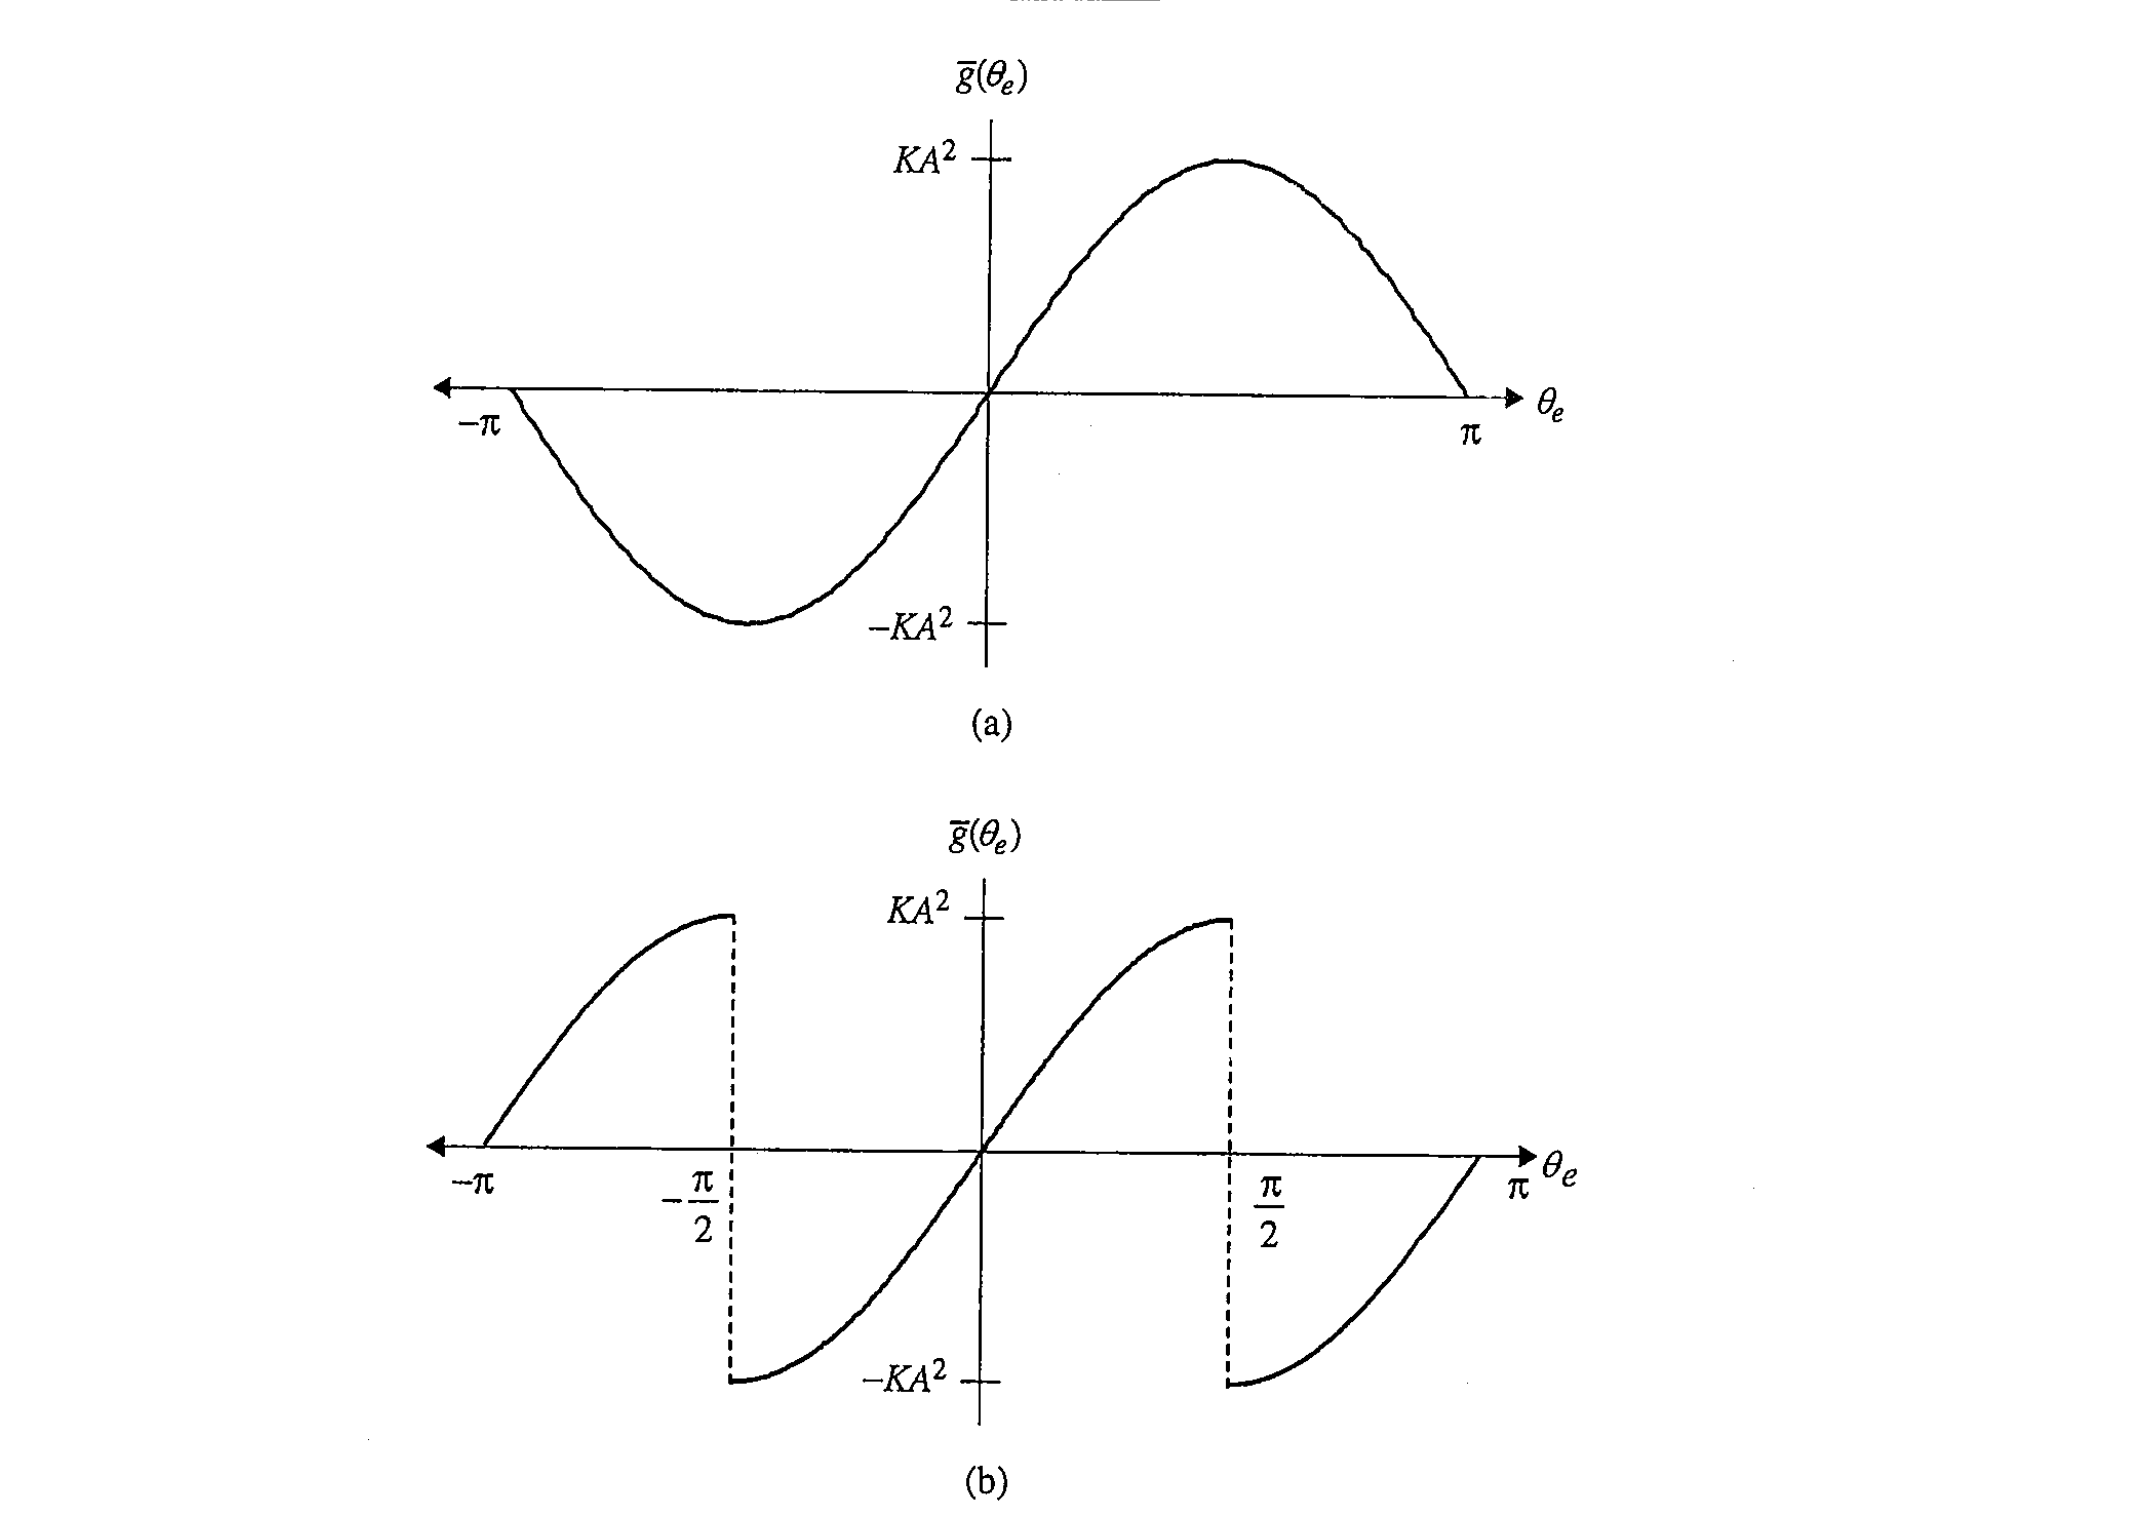
\includegraphics[width=\textwidth]{s_curve_bpsk}
  \caption{S-curves for the a) data-aided BPSK phase detector and b) the decision-directed BPSK phase detector [\citeauthor{digcomm_discrete_approach}]}
  \label{fig:s_curve_bpsk}
\end{figure}

Note the detector gain is dependent on the input sinal amplitude $K$ and so it's common to pass the input signal through a block such as an AGC, that adjusts the amplitude to the required value. Also note that the decision-directed QPSK case has 4 stable lock points (crosses zero with a positive slope), resulting in a $\frac{\pi}{2}$ phase ambiguity:
\begin{equation}
  \theta_e=-\frac{\pi}{2},0,\frac{\pi}{2},\pi
\end{equation}

Similarly, the BPSK case has 2 stable lock points ($\theta_e=0,\pi$), resulting in a $\pi$ phase ambiguity.

As for the remaining parameters, the damping factor $\zeta$ and the normalized loop bandwidth $B_nT$ are usually chosen by the designer to obtain the desired performance (a critically damped system is a popular choice). $K_0$, the DDS sensitivity, is usually taken to be 1. the remaining parameters $K_1$ and $K_2$ can be calculated given the two expressions previously given for the loop constants in \eqref{eq:digital_loop_constants1} and \eqref{eq:digital_loop_constants2}.

To conclude, an example of loop design with the ML detector is shown. Suppose the requirements specify QPSK modulation, an equivalent loop bandwidth of 2\% of the symbol rate ($B_n=0.02$) and a damping factor $\zeta=\frac{1}{\sqrt{2}}$. Assume for simplicity that $KA^2=1$ and also $K_0=1$. In this case, the proportional-plus-integrator loop filter constants are $K_1=2.6\times10^{-2}$ and $K_2=6.9\times10^{-4}$.

\autoref{fig:demo_fsync} show a Jupyter notebook example using the \code{FrequencySync} module to synchronize a QPSK signal embedded in AWGN noise and with an introduced phase and frequency offset.

\begin{figure}[ht]
  \centering
  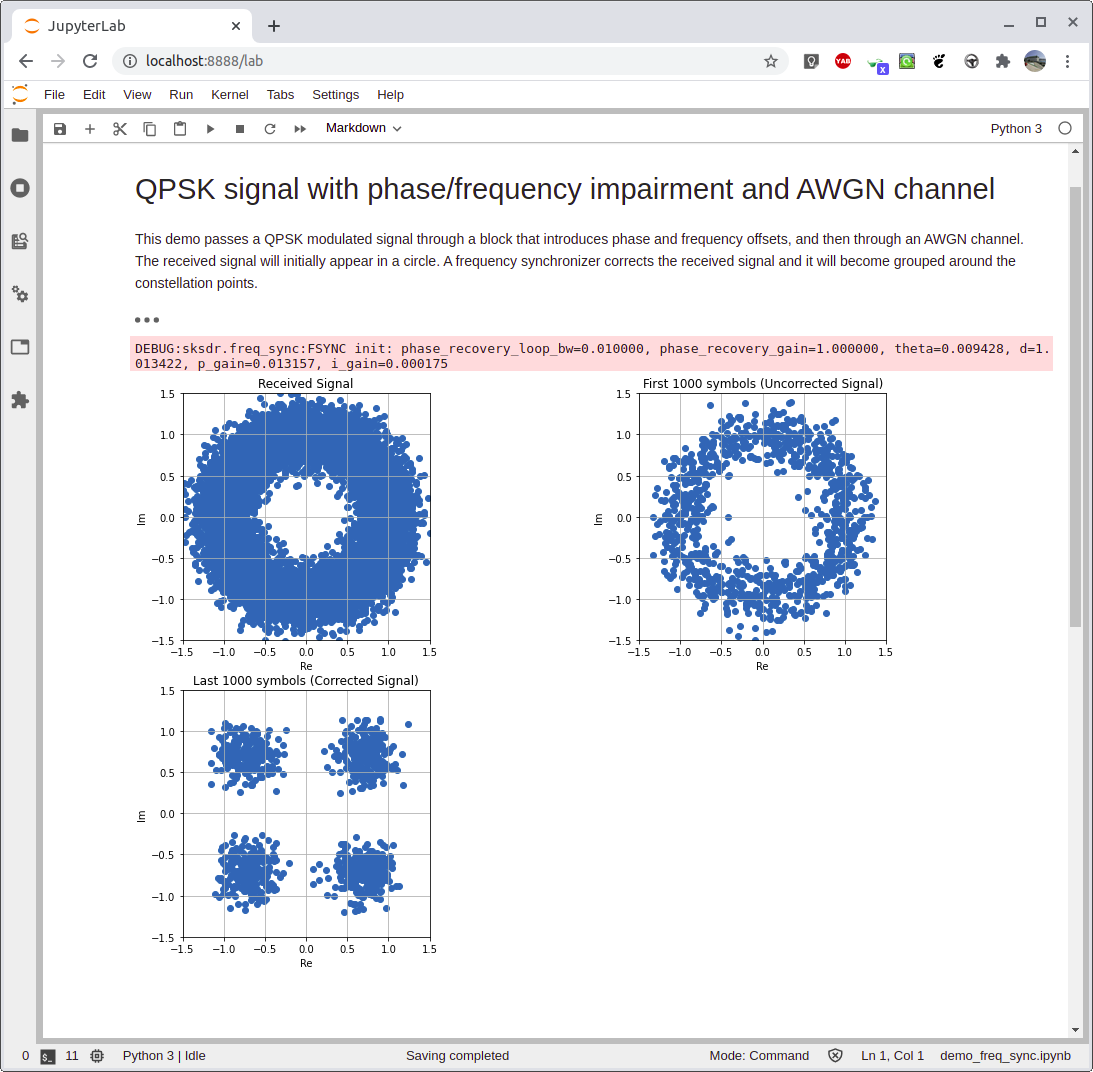
\includegraphics[width=0.75\textwidth]{demo_fsync}
  \caption{\code{FrequencySync} Jupyter notebook demonstration}
  \label{fig:demo_fsync}
\end{figure}

%%%%%%%%%%%%%%%%%%%%%%%%%%%%%%%%%%%%%%%%%%%%%%%%%%%%%%%%%%%%%%%%%%%%%%%%%%%%%%%
\section{Symbol Timing Synchronizer (PLL based)}

The \code{SymbolSync} module corrects symbol timing clock skew between a single-carrier transmitter and receiver. Currently it supports BPSK and QPSK modulation schemes.

\noindent Module properties:
\begin{itemize}
  \item \code{sps}: Samples per symbol of the input signal
  \item \code{mod}: Modulation of the input signal
  \item \code{damp\_factor}: PLL's damping factor
  \item \code{norm\_loop\_bw}: PLL's normalized loop bandwidth
  \item \code{K}: Input signal amplitude
  \item \code{A}: Symbol magnitude
\end{itemize}

Symbol timing synchronization consists of estimating a clock signal that is aligned in phase and frequency with the clock used to generate the data sequence at the transmitter. The clock is extracted from the (possibly noisy) received waveforms that carry the data and this estimate is used to identify the instants when the matched filter output should be sampled. \autoref{fig:drawing_sym2} shows the structure of the symbol timing synchronizer.

\begin{figure}[H]
  \centering
  \includegraphics[width=0.75\textwidth]{drawing_sym2}
  \caption{Discrete-time approach to symbol timing synchronization for sampled-data detectors}
  \label{fig:drawing_sym2}
\end{figure}

The algorithm is based on a discrete-time PLL algorithm, which consists of four components \cite{digcomm_discrete_approach}:
\begin{itemize}
  \item A timing error detector (TED)
  \item An interpolator
  \item An interpolation controller
  \item A loop filter
\end{itemize}

In terms of a discrete-time PLL structure, the interpolator and TED combination are the phase detector, and the interpolator control is the DDS. For more information, refer to \autoref{sect:library_freq_sync}, where an in-depth explanation of discrete-time PLL workings and parameters is presented.

Having a purely discrete-time architecture solves many of the problems associated with the continuous-time or hybrid approaches, such as phase noise on the voltage controlled clock (VCC) that drives the ADC. This however means that the ADC is not part of the loop and so the received signal $r(t)$ is sampled at a fixed rate $\frac{1}{T}$, that is asynchronous to the symbol rate $\frac{1}{T_s}$. As a consequence, this approach produces samples which are not aligned with the symbol boundaries. The role of the symbol timing synchronization is to `move' the samples to the desired time instants. Another name for `moving' samples in time is \emph{interpolation}. Because the synchronizer has to adapt to an unknown time delay, the interpolator needs to be adaptive. When working correctly, the interpolator produces matched filter outputs which are aligned with the symbols boundaries and the optimum sampling instant.

\subsection{Timing Error Detector}
\label{sect:timing_error_detector}

In general the detector produces an error signal once every symbol based on the current timing estimate $\hat \tau$ and the output of the matched filter $x(nT)$. The interpolator computes the interpolant $x(kT_s+\hat \tau)$ as:
\begin{equation}
x(kT_s+\hat\tau) = K\sum_{m} a(m)r_p\left(\left(k-m\right)T_s-\tau_e\right)
\end{equation}

where $\tau_e=\tau-\hat\tau$ is the timing error, $r_p$ is the autocorrelation function of the pulse shaping filter and $T_s$ is symbol period. The TED then produces a signal $g(\tau_e)$ that is a function of this timing error, in the same way the phase detector in a carrier frequency synchronizer produces a signal that is a function of the phase error. The characteristics of a TED, similarly to a phase error detector (PED), are described by its S-curve.

There are several TEDs in the literature and for this module the \emph{zero crossing TED} (ZCTED) has been chosen. It's a \emph{decision-directed} TED that offers similar performance to other alternatives, such as the \emph{maximum likelihood} TED (MLTED) and the \emph{early-late} TED (ELTED), but it is less susceptible to self-noise. This detector is based on finding the zero crossings in the eye diagram as opposed to the MLTED and ELTED which rely on the slope of the eye diagram. It operates at 2 samples/second and provides zero error when every other sample is time-aligned with a zero crossing in the matched filter output (the other samples are then time-aligned with the optimum sampling instants corresponding to maximum average eye opening). \autoref{fig:zero_crossing_detector} illustrates the operation of the ZCTED.

\begin{figure}[ht]
  \centering
  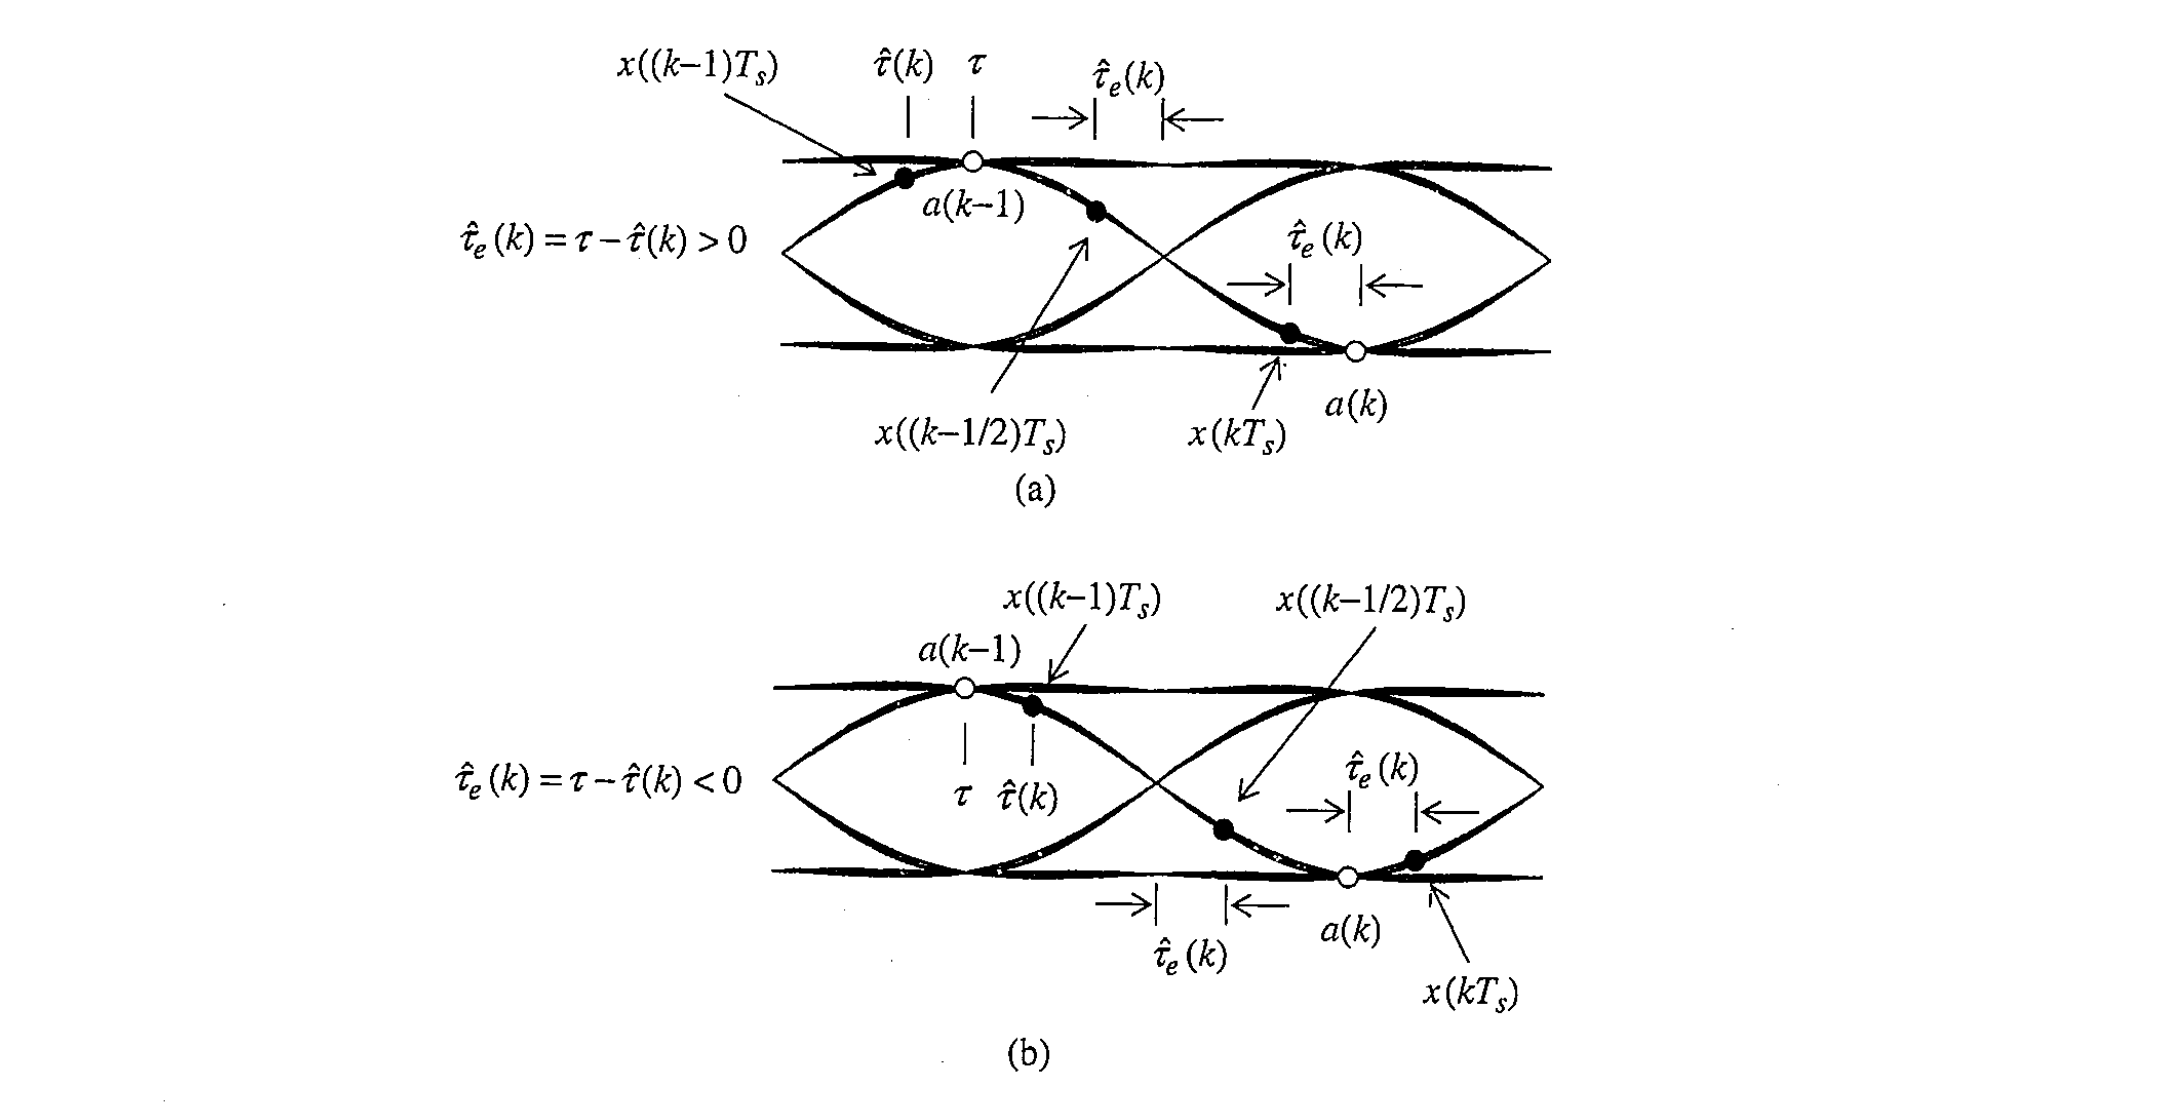
\includegraphics[width=\textwidth]{zero_crossing_detector}
  \caption{Operation of the zero-crossing TED. a) the timing estimate is early, b) the timing estimate is late [\citeauthor{digcomm_discrete_approach}]}.
  \label{fig:zero_crossing_detector}
\end{figure}

It can be shown \cite{digcomm_discrete_approach} that the error signal of the ZCTED is
\begin{equation}
e(k) = x\left(\left(k-1/2\right)T_s+\hat\tau\right)\left[\hat a\left(k-1\right)-\hat a\left(k\right)\right]
\end{equation}
where $\hat a(k)$ are the symbol estimates (for the decision-directed case), given by
\begin{align}
\hat a(k-1) &= A\times\operatorname{sgn}\left(x\left(\left(k-1\right)T_s + \hat\tau\right)\right)\\
\hat a(k)   &= A\times\operatorname{sgn}\left(x\left(\left(k\right)T_s + \hat\tau\right)\right)
\end{align}

An alternative is to use
\begin{align}
\hat a(k-1) &= \operatorname{sgn}\left(x\left(\left(k-1\right)T_s + \hat\tau\right)\right)\\
\hat a(k)   &= \operatorname{sgn}\left(x\left(\left(k\right)T_s + \hat\tau\right)\right)
\end{align}

This approximation provides the proper sign but not the proper amplitude for the estimation. This, however, does not appear to impact performance in any significant way.

The S-curve for the ZCTED can be obtained computing the expected value of $e(k)$ and assuming the symbols are uncorrelated. This can be shown to be
\begin{equation}
g(\tau_e)=K\cdot E_{avg}\left[ r_p\left(T_s/2-\tau_e\right) - r_p\left(-T_s/2-\tau_e\right) \right]
\end{equation}

The gain of the ZCTED, $K_p$, is the slope of $g(0)$ and is proportional to the received signal amplitude $K$ and the average symbol energy $E_{avg}$. This poses the same challenges as for the carrier frequency synchronization module, in the sense that $K$ must be either estimated and $K_p$ updated dynamically, or in alternative, $K$ must be kept within restricted values by use of an AGC block, for example. Finally because $r_p$ is a function of the pulse shaping filter, $K_p$ is also a function of the excess bandwidth, for the case of the root raised cosine filter.

\subsection{Interpolation}

The fundamental interpolation equation may be derived by considering a fictitious system involving continuous-time processing as illustrated in \autoref{fig:interpolation_dac}.

\begin{figure}[H]
  \centering
  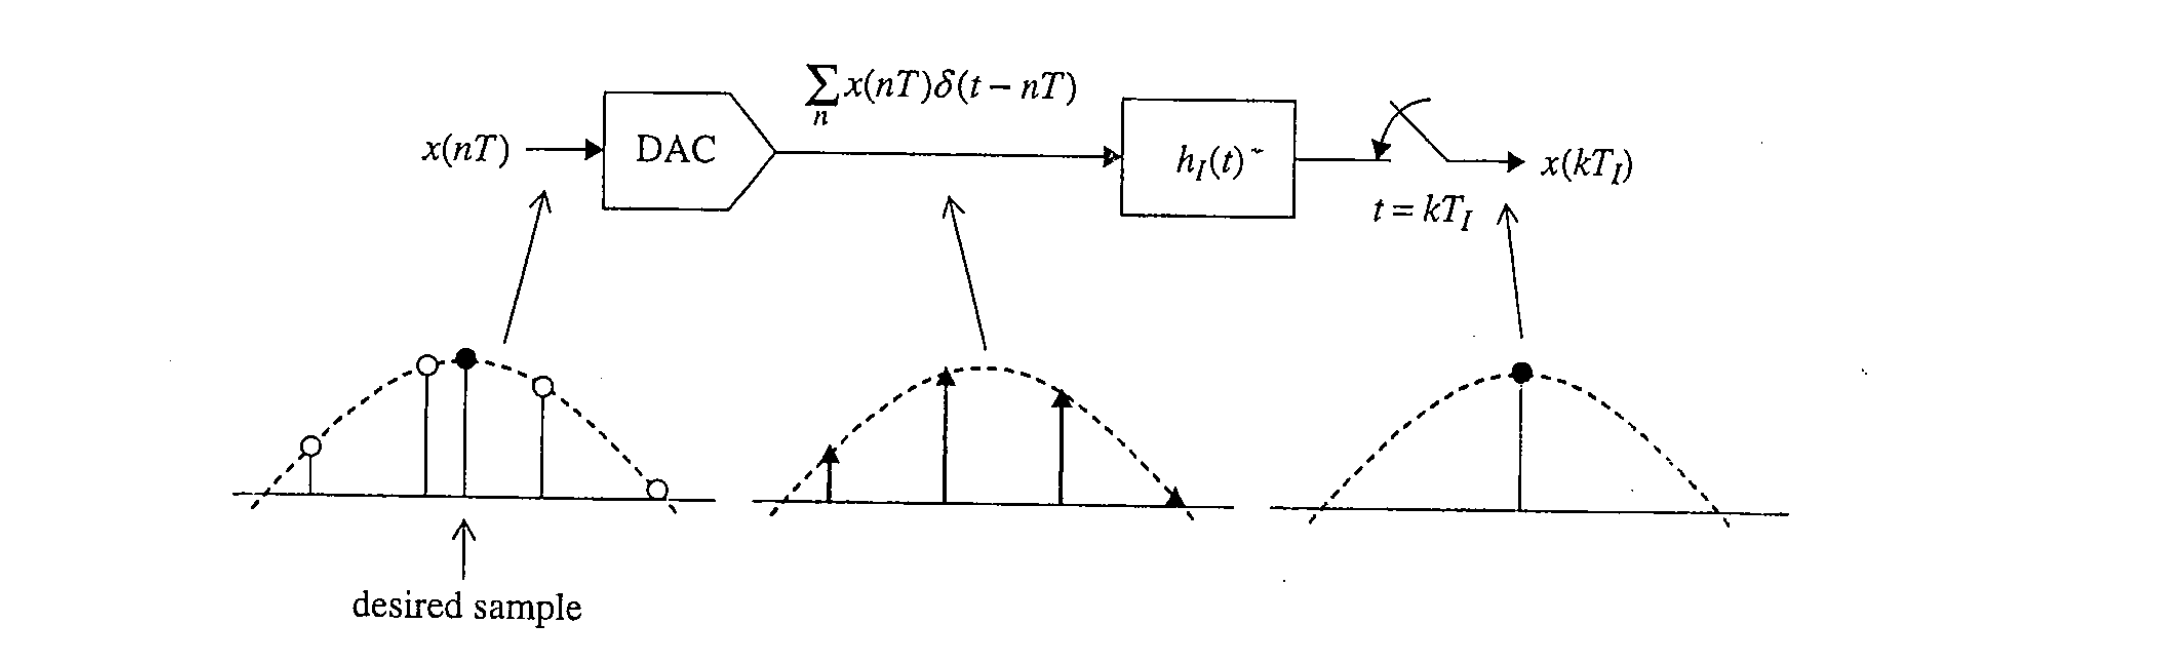
\includegraphics[width=\textwidth]{interpolation_dac}
  \caption{Ficticious system using continuous-time processing for performing interpolation [\citeauthor{digcomm_discrete_approach}]}
  \label{fig:interpolation_dac}
\end{figure}

First the input samples $x(nT)$ are converted to a weighted impulse train by the DAC. This impulse train is then filtered by an interpolation filter with impulse response $h_I(t)$ to produce the continuous time signal $x(t)$. Finally, to produce the desired samples, $x(t)$ is resampled at intervals $kT_I$ ($k=0,1,\ldots)$:
\begin{equation}
x(kT_I)=\sum_{n} x(nT)h_I(kT_I-nT)
\end{equation}

The desired sample, $x(kT_I)$, is called the $k$-th \emph{interpolant}. When the $k$-th interpolant is between samples $x(nT)$ and $x((n+1)T)$, the sample index $n$ is called the $k$-th \emph{basepoint index}, denoted by $m(k)$ and defined by $m(k)=\lfloor kT_I/T \rfloor$. The time instant $kT_I$ is some fraction of a sample time greater than $m(k)T$ and this fraction is called the $k$-th \emph{fractional interval}, denoted $\mu(k)$ and defined by $\mu(k)T=kT_I-m(k)T$. The previous expression for $x(kT_I)$ can be expressed in terms of these definitions using the filter index $i=m(k)-n$:
\begin{equation}
x(kT_I)=\sum_{i} x\left(\left(m(k\right)-i\right)T)h_I\left(\left(i+\mu\left(k\right)\right)T\right)
\end{equation}

\autoref{fig:interpolation} illustrates the principles behind the interpolation process.

\begin{figure}[H]
  \centering
  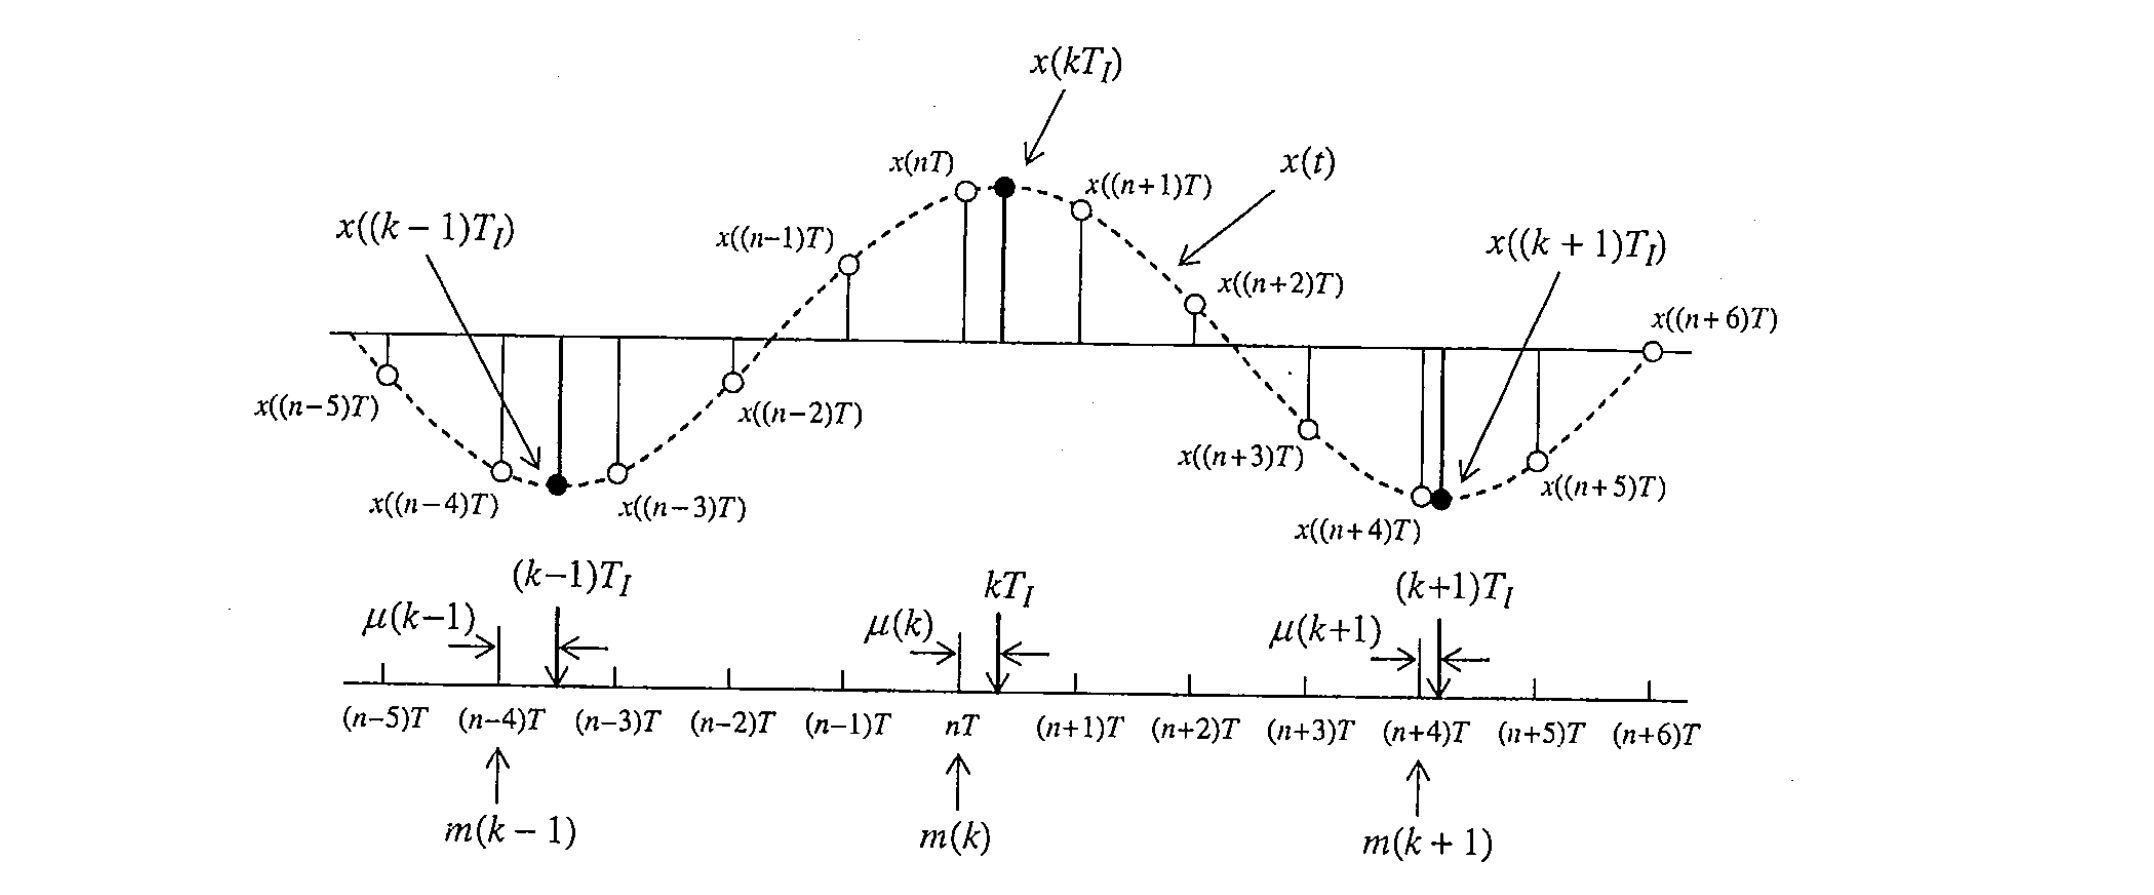
\includegraphics[width=\textwidth]{interpolation}
  \caption{Illustration of the relationships between the intepolation interval $T_I$, the sample time $T$, the basepoint indexes, and the fractional intervals [\citeauthor{digcomm_discrete_approach}]}
  \label{fig:interpolation}
\end{figure}

The optimum interpolation filter is an ideal low-pass filter with impulse response:
\begin{equation}
h_I(t)=\frac{\sin(\pi t/T)}{\pi t/T}
\end{equation}

Since this is unrealizable, one choice would be to massively upsample the matched filter input, match filter at the high sample rate and then downsample the output with the appropriately chosen sample offset. This is often denoted by a \emph{polyphase filterbank interpolator}. This technique is out of scope for this thesis and so will not be discussed. Another popular alternative is a class of FIR filters which approximate the ideal response, known as \emph{piecewise polynomial filters}. First, the underlying continuous waveform $x(t)$ is approximated by a polynomial in $t$:
\begin{equation}
x(t)\approx c_pt^p+c_{p-1}t^{p-1}+\ldots+c_1t+c_0
\end{equation}

Once the coefficients are known, the interpolant at $t=kT_I=\left(m(k)+\mu(k)\right)T$ is obtained by
\begin{equation}
x(kT_I)\approx c_p(kT_I)^p+c_{p-1}(kT_I)^{p-1}+\ldots+c_1(kT_I)+c_0
\end{equation}

When p = 1, this becomes
\begin{equation}
x((m(k)+\mu(k))T)=c_1((m(k)+\mu(k))T) + c_0
\end{equation}

The coefficients are determined by the available samples and satisfy
\begin{equation}\begin{bmatrix}
x(m(k)T)\\
x((m(k)+1)T)
\end{bmatrix}
=
\begin{bmatrix}
m(k)T & 1\\
(m(k)+1)T & 1
\end{bmatrix}
\begin{bmatrix}
c_1\\
c_0
\end{bmatrix}
\end{equation}

Solving for $c_0$ and $c_1$ gives
\begin{equation}
x((m(k)+\mu(k))T) = \mu(k)x((m(k)+1)T)+(1-\mu(k))x(m(k)T)
\end{equation}
which the linear interpolator.

There are four important observations:
\begin{enumerate}
  \item The interpolant is a linear combination of the available samples. As a consequence, it can thought of the output of an equivalent filter with coefficients
  \begin{equation}
  x((m(k)+\mu(k))T) = \sum_{i=-1}^{0}h_1(i)x((m(k)-i)T)
  \end{equation}
  where
  \begin{align}
  h_1(-1) &= \mu(k)\\
  h_1(0) &= 1 - \mu(k)
  \end{align}

  \item The equivalent filter coefficients are a function of the fractional interval $\mu(k)$ and not the base point $m(k)$. This is important to avoid overflow on the coefficients from the increasing base point index.

  \item The interpolating filter is a linear phase FIR filter, an important property. This can be seen because the coefficients are symmetric around the centre point of the filter $\mu(k) = 1/2$ and is a result of using an even number of samples to compute an interpolant that is between the middle two. It however poses a restrictions of using even number of coefficients and therefore an odd-degree polynomial.

  \item The sum of the coefficients is 1, and therefore independent of $\mu(k)$. This means the filter doesn't change the amplitude of the underlying waveform in the process of computing the interpolant.
\end{enumerate}

Having established the structure of piecewise polynomial approximation, a $p=2$ (second degree) polynomial is chosen, which is called a \emph{parabolic interpolator}. Given observation 3 though, it will have an additional parameter $\alpha$ to account for the extra degree of freedom introduced by having to use 4 points instead of 3. In the same way it was done for the linear interpolator, it can be shown that the coefficients of the equivalent filter in this case are

\begin{align}
h_3(-2) &= \alpha\mu(k)^2-\alpha\mu(k) \\
h_3(-1) &= -\alpha\mu(k)^2+(1+\alpha)\mu(k) \\
h_3(0) &= -\alpha\mu(k)^2-(1-\alpha)\mu(k)+1 \\
h_3(1) &= \alpha\mu(k)^2-\alpha\mu(k)
\end{align}

Using a piecewise polynomial interpolator to produce the interpolant will result in a computation of the form
\begin{equation}
x((m(k)+\mu(k))T)=\sum_{i=-I_1}^{I_2}h_p(i;\mu(k))x((m(k)-i)T)
\end{equation}
which is an approximation to the ideal filter response $h_I(t)$ defined earlier.

Because the coefficients $h_p$ are a function of $\mu(k)$, a hardware implementation requires 2-input multipliers with variable inputs. It can be shown that this can be optimized into a structure of the form
\begin{equation}
x((m(k)+\mu(k))T)=\sum_{l=0}^{p}\mu(k)^l\underbrace{\sum_{i=I_1}^{I_2} b_l(i)x((m(k)-i)T)}_{v(l)}
\end{equation}

In this form the inner sum becomes a filter equation in which the input data samples $x((m(k)-i)T)$ pass through a filter with impulse response $b_l(i)$. These coefficients are independent of $\mu(k)$. This can be further simplified by nested evaluation to the following structure, called a \emph{Farrow structure}\cite{farrow1988}, for a piecewise parabolic interpolator:
\begin{equation}
x((m(k)+\mu(k))T)=(v(2)\mu(k)+v(1))\mu(k)+v(0)
\end{equation}

The \emph{Farrow coefficients} for this interpolator are listed in \autoref{table:farrow_coeffs}.
\begin{table}[ht]
  \caption{Farrow coefficients for a piecewise parabolic interpolator}
  \label{table:farrow_coeffs}
  \centering
  \begin{adjustbox}{}
  \begin{tabular}{r | r | r | r}
  \toprule
  \thead{$i$} & \thead{$b_2(i)$} & \thead{$b_1(i)$} & \thead{$b_0(i)$} \\
  \hline
  $-2$ & $\alpha$ & $-\alpha$ & 0 \\
  $-1$ & $-\alpha$ & $1+\alpha$ & 0 \\
  $0$ & $-\alpha$ & $\alpha-1$ & 1 \\
  $1$ & $\alpha$ & $-\alpha$ & 0 \\
  \end{tabular}
  \end{adjustbox}
\end{table}

\subsection{Interpolator Control}

The function of interpolator control is to provide the interpolator with $k$-th basepoint $m(k)$ and the $k$-th fractional interval $\mu(k)$. One of the common methods for interpolator control, and used in this module, is the \emph{modulo-1 counter}. \autoref{fig:drawing_modulo_counter} shows its block diagram and \autoref{fig:modulo-1} illustrates the interpolation process from a time perspective.

\begin{figure}[H]
  \centering
  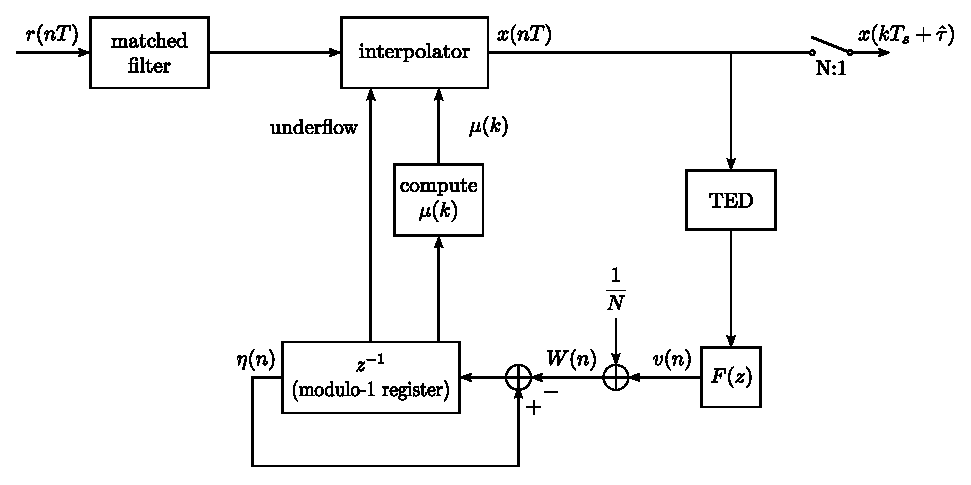
\includegraphics[width=\textwidth]{drawing_modulo_counter}
  \caption[Modulo-1 counter for interpolation control]{Modulo-1 counter for interpolation control. The basepoint index is identified by the underflow strobe and the fractional interval updated using the counter contents on underflow.}
  \label{fig:drawing_modulo_counter}
\end{figure}

\begin{figure}[H]
  \centering
  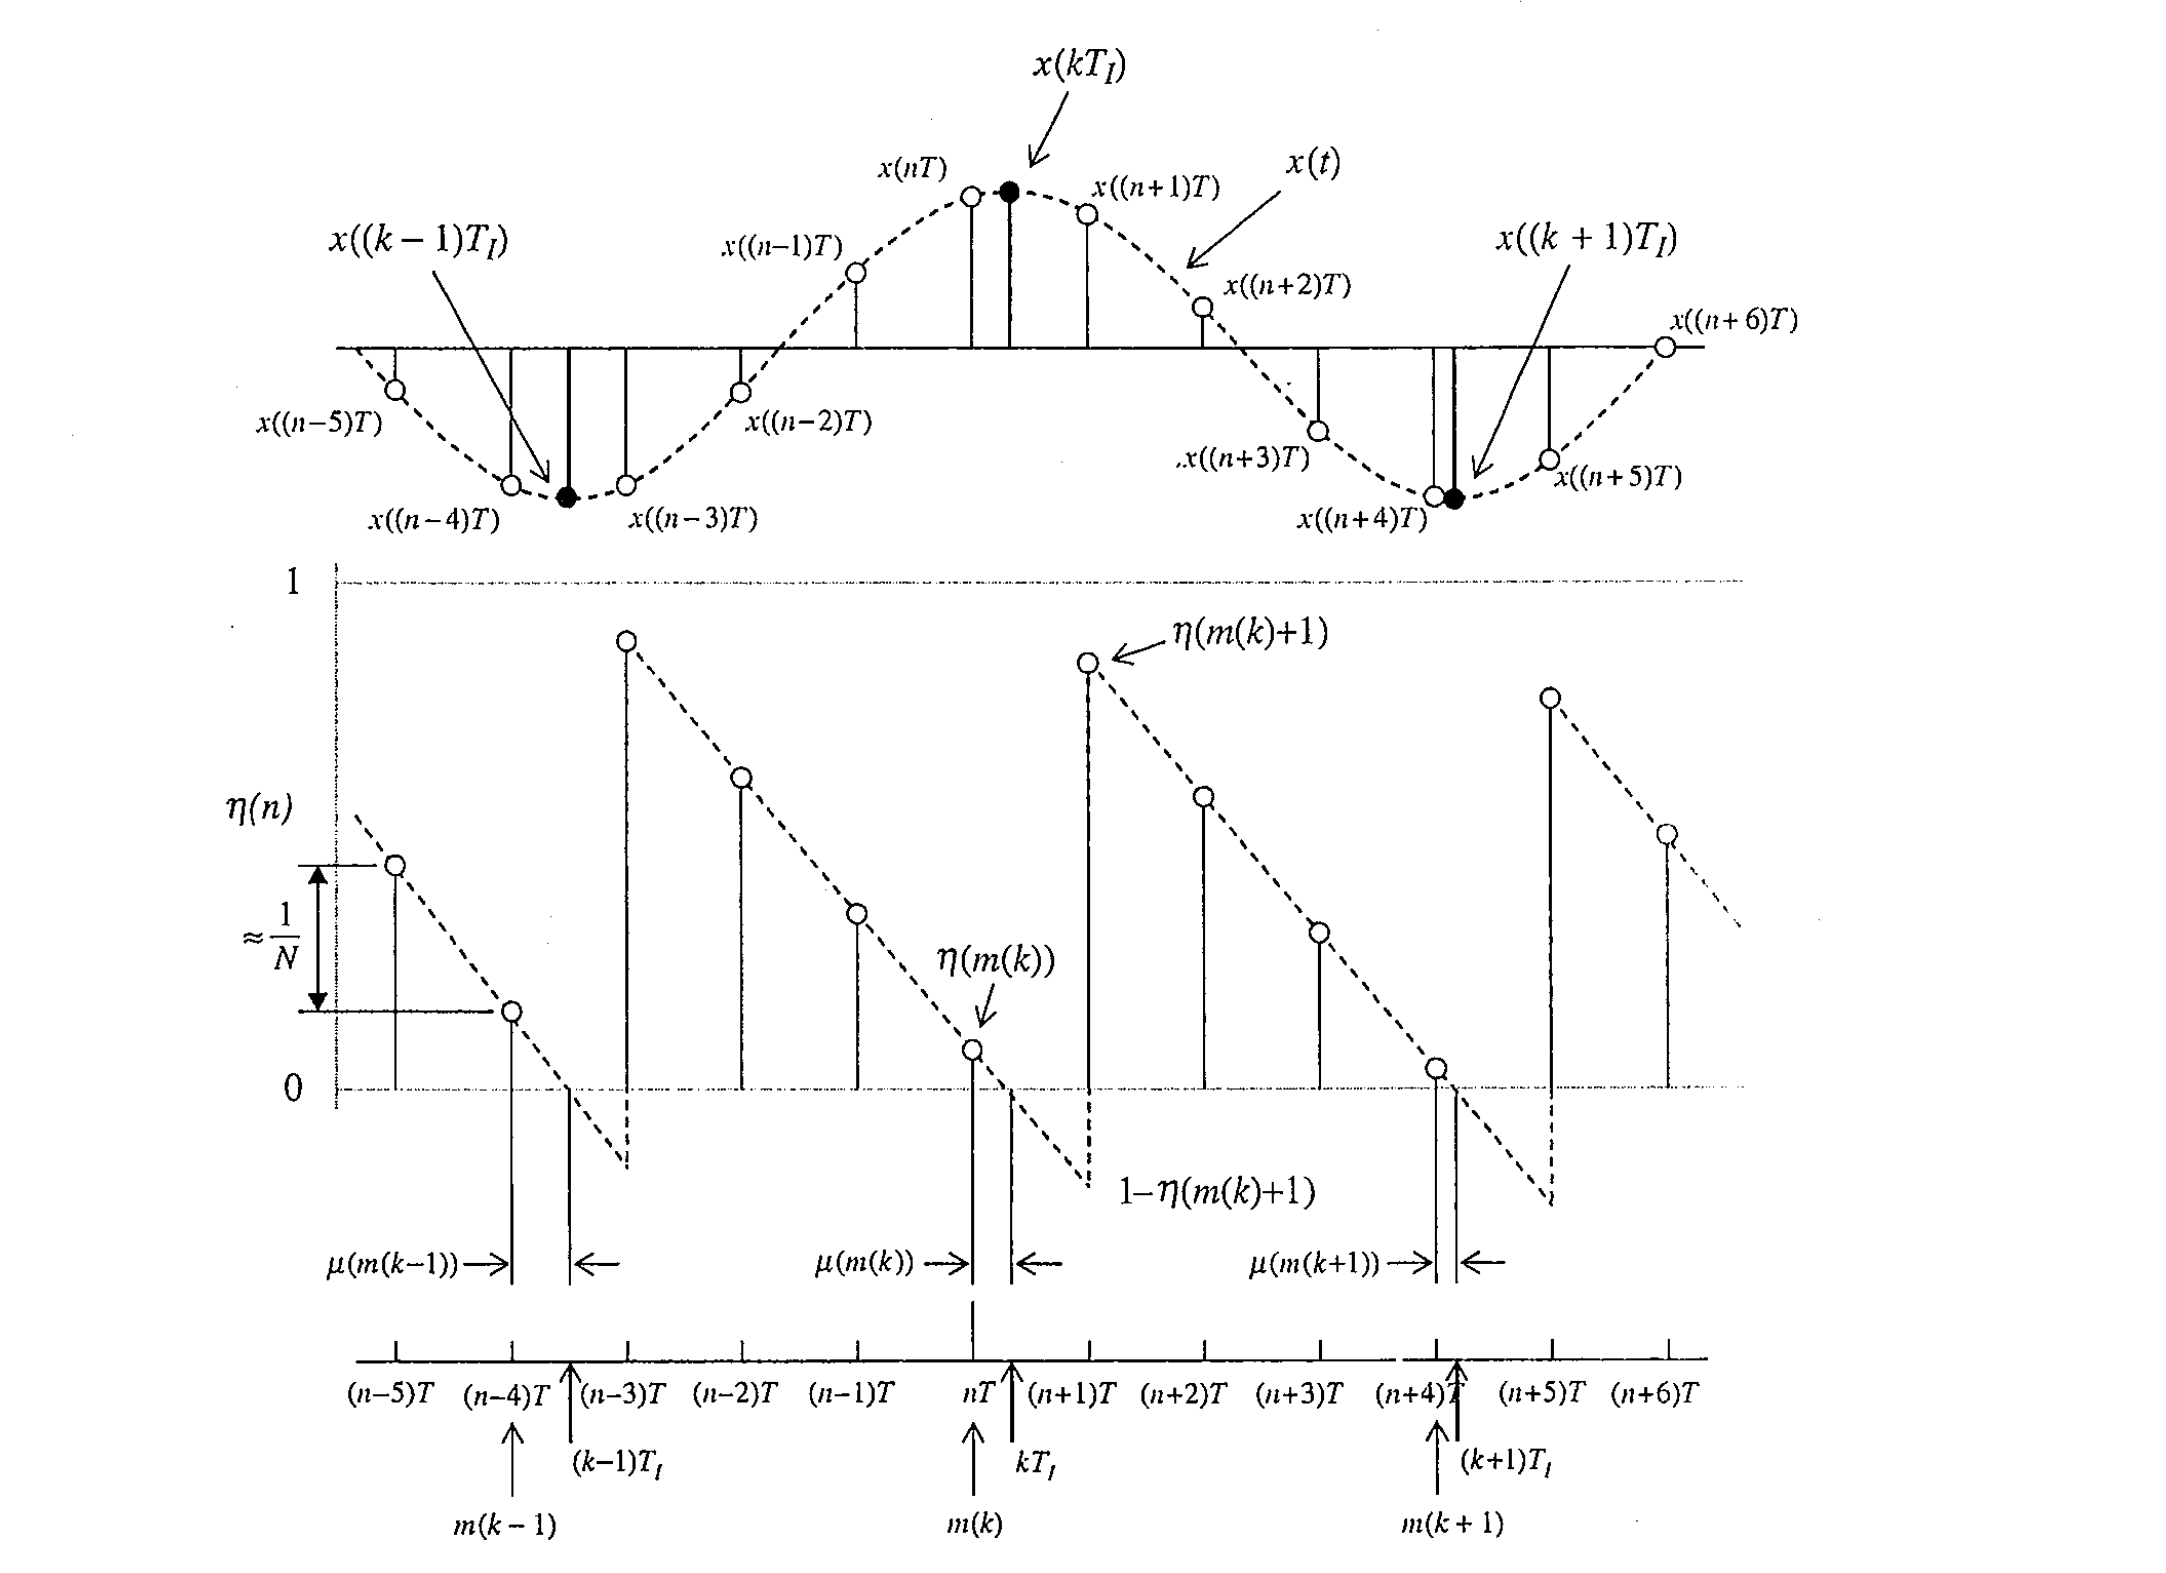
\includegraphics[width=\textwidth]{modulo-1}
  \caption{Illustration of the relationship between the available samples, the desired interpolants and the modulo-1 counter contents [\citeauthor{digcomm_discrete_approach}]}
  \label{fig:modulo-1}
\end{figure}

The counter decrements by $1/N$ so that the underflows occur every $N$ samples. The loop filter output $v(n)$ adjusts the amount by which the counter decrements. When operating correctly the underflow occurs 1 sample after the desired interpolant. The underflow condition is indicated by a \emph{strobe} and used by the interpolator to identify the basepoint index. The fractional interval is obtained from the contents of the modulo-1 counter on underflow. In general, the counter values satisfies the recursion
\begin{equation}
\eta(n+1)=\left(\eta(n)-W(n)\right)\operatorname{mod}1
\end{equation}
where $W(n)=1/N+v(n)$. When the decrementing counter underflows, the index $n$ is the basepoint index $m(k)$. Incorporating the modulo-1 reduction produces
\begin{equation}
  \eta\left(m(k)+1\right)=1+\eta\left(m(k)\right)-W\left(m(k)\right)
\end{equation}

As illustrated in \autoref{fig:modulo-1}, the counter values $\eta(m(k))$ and $1-\eta(m(k)+1)$ for similar triangles. This observation leads to the relationship
\begin{equation}
\frac{\mu(m(k))}{\eta(m(k))}=\frac{1-\mu(m(k))}{1-\eta((m(k)+1))}
\end{equation}

Solving for $\mu(m(k))$ gives
\begin{equation}
\mu(m(k))=\frac{\eta(m(k))}{W(m(k))}
\end{equation}

The underflow period (in samples) is
\begin{equation}
\frac{1}{W(n)}=\frac{N}{1+Nv(n)}
\end{equation}

When in lock, $v(n)$ is zero on average, and the decrementing modulo-1 counter underflow period is $N$ samples on average. During acquisition, $v(n)$ aligns the underflow periods to align the symbol boundaries. The decrementing modulo-1 counter plays the same role in this system as the DDS plays in a phase/frequency synchronization PLL and its modulo-1 operation corresponds to the modulo-$2\pi$ operation of the DDS. Noting that the gain $K_0$ is $-1$ in this case, instead of $1$, because it's a decrementing counter.

\autoref{fig:demo_symbol_sync} show a Jupyter notebook example using this module to synchronize a QPSK signal embedded in AWGN noise and with an introduced timing delay.

\begin{figure}[H]
  \centering
  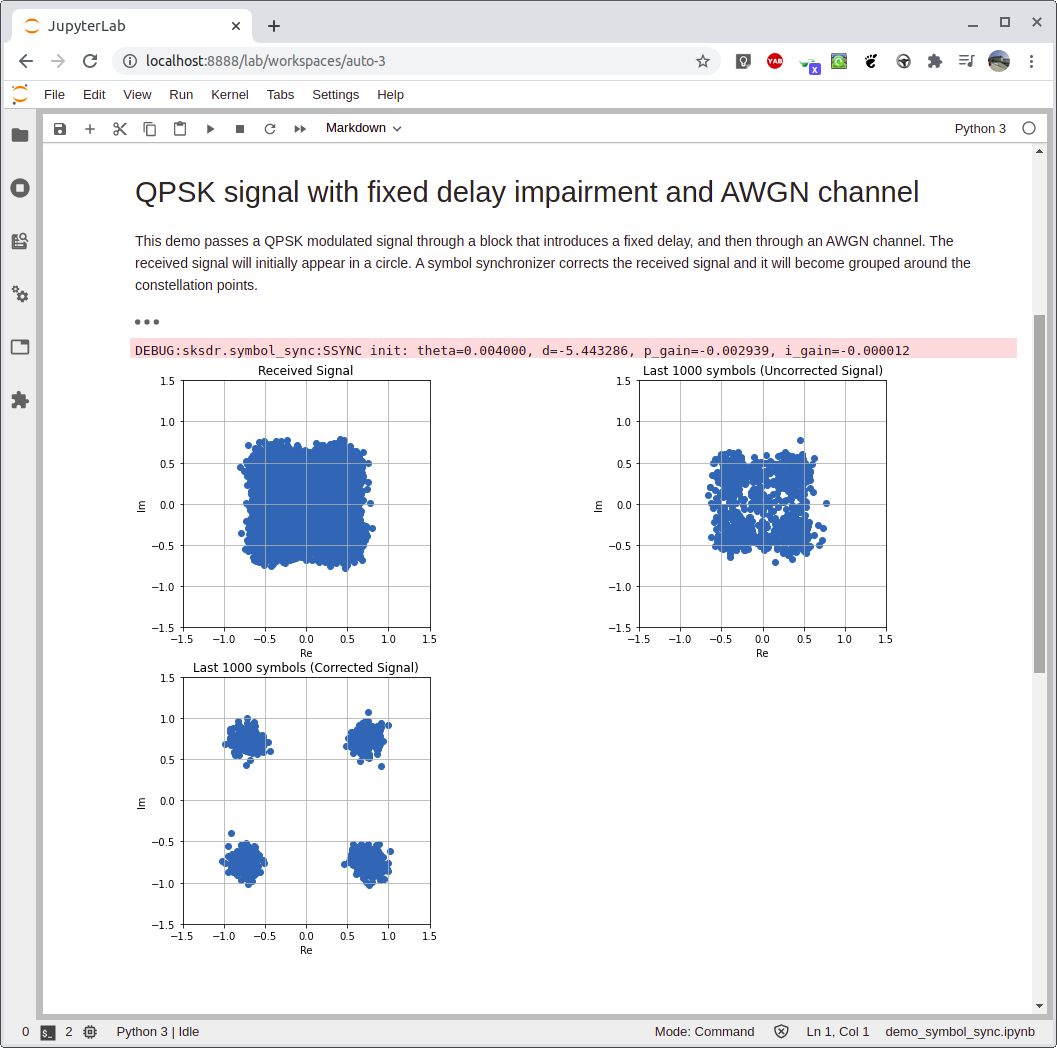
\includegraphics[width=0.75\textwidth]{demo_symbol_sync}
  \caption{\code{SymbolSync} Jupyter notebook demonstration}
  \label{fig:demo_symbol_sync}
\end{figure}

%%%%%%%%%%%%%%%%%%%%%%%%%%%%%%%%%%%%%%%%%%%%%%%%%%%%%%%%%%%%%%%%%%%%%%%%%%%%%%%
\section{Automatic Gain Control}

The AGC module adaptively adjusts its gain to achieve a constant output power.

\noindent Module properties:
\begin{itemize}
  \item \code{ref\_power}: Desired output power
  \item \code{max\_gain} (dB): Upper limit on the loop gain
  \item \code{det\_gain}: Detector gain
  \item \code{avg\_len} (samples): Length of moving average filter
\end{itemize}

The module doesn't use a linear loop scheme since that has a significant drawback: The time constant of the loop is input signal level dependent, and is different depending on whether the input signal is increasing or decreasing. These properties drastically reduce the control over the system's time constant. To solve this problem, a logarithmic loop is adopted. This allows control of the AGC's time constant, increases its dynamic range and generally provides good performance for a variety of signal types. \autoref{fig:agc_diagram} shows a block diagram of the algorithm.

% \begin{figure}[ht]
% \centering
% \begin{tikzpicture} [circuit ee IEC,
%                       small circuit symbols,
%                       every info/.style={font=\footnotesize},
%                       set make contact graphic= var make contact IEC graphic,
%                       skip loop/.style={to path={-- ++(0,-1) -| (\tikztotarget)}},
%                       skip loop left/.style={to path={-- ++(-1,0) |- (\tikztotarget)}}]

% \matrix (m1) [row sep=10mm, column sep=10mm]
% {
%   %--------------------------------------------------------------------
%   \node[dspnodeopen,dsp/label=above] (m00) {$x(n)$}; &
%   \node[dspmixer] (m01) {}; &
%   \node[coordinate] (m02) {1}; &
%   \node[coordinate] (m03) {2}; &
%   \node[coordinate] (m04) {}; &
%   \node[coordinate] (m05) {}; &
%   \node[coordinate] (m06) {}; &
%   \node[coordinate] (m07) {}; &
%   \node[dspnodefull] (m08) {}; &
%   \node[dspnodeopen,dsp/label=above] (m09) {$y(n)$}; \\
%   %--------------------------------------------------------------------
%   \node[coordinate] (m10) {}; &
%   \node[dspsquare] (m11) {$\exp$}; &
%   \node[coordinate] (m12) {}; &
%   \node[coordinate] (m13) {}; &
%   \node[dspnodeopen,dsp/label=above] (m14) {$K$}; &
%   \node[dspnodeopen,dsp/label=above] (m15) {$\ln(A)$}; &
%   \node[coordinate] (m16) {}; &
%   \node[coordinate] (m17) {}; &
%   \node[dspmixer] (m18) {}; &
%   \node[coordinate] (m19) {}; \\
%   %--------------------------------------------------------------------
%   \node[coordinate] (m20) {}; &
%   \node[dspnodefull] (m21) {}; &
%   \node[dspsquare] (m22) {$z^{-1}$}; &
%   \node[dspadder] (m23) {}; &
%   \node[dspmixer] (m24) {}; &
%   \node[dspadder] (m25) {}; &
%   \node[dspsquare] (m26) {$\ln$}; &
%   \node[dspsquare,inner xsep=1mm] (m27) {LPF}; &
%   \node[coordinate](m28) {}; \\
% };

% \begin{scope}[start chain]
%   \chainin (m00);
%   \chainin (m01) [join=by dspconn];
%   \chainin (m08) [join=by dspflow];
%   \chainin (m09) [join=by dspconn];
% \end{scope}

% \begin{scope}[start chain]
%   \chainin (m08) [join=by dspconn];
%   \chainin (m18) [join=by dspconn];
%   \chainin (m28) [join=by dspline];
%   \chainin (m27) [join=by dspconn];
%   \chainin (m26) [join=by dspconn];
%   \chainin (m25) [join=by dspconn];
%   \chainin (m24) [join=by dspconn];
%   \chainin (m23) [join=by dspconn];
%   \chainin (m22) [join=by dspconn];
%   \chainin (m21) [join=by dspline];
%   \chainin (m11) [join=by dspconn];
%   \chainin (m01) [join=by dspconn];
% \end{scope}

% \draw[dspconn] (m14) to (m24);
% \draw[dspconn] (m15) to (m25);
% \path (m21.south)
%   edge[dspconn,skip loop] (m23.south);
% \path ($ (m08) + (0,-2mm) $)
%   edge[dspconn,skip loop left] (m18.west);
% \draw[dspline] (m26) -- node[near end,below] {$-$} (m25);

% \end{tikzpicture}
% \caption{AGC diagram}
% \label{fig:agc_diagram}
% \end{figure}

\begin{figure}[H]
  \centering
  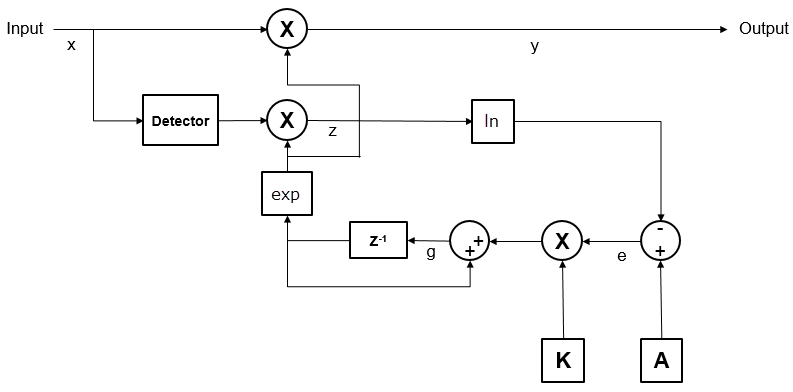
\includegraphics[width=0.80\textwidth]{agc_diagram}
  \caption{AGC block diagram [\citeauthor{mathworks_agc}]}
  \label{fig:agc_diagram}
\end{figure}

The detector block is composed of a low-pass filter (LPF) to eliminate rapid gain changes. That filter can be a simple moving average filter, a cascaded integrator-comb (CIC) filter, or a more traditional low-pass filter having a sinc-shaped impulse response. In the current implementation, a moving average filter is implemented, which computes the average power of the last \code{avg\_len} samples. This power is then multiplied by the loop gain $g(n)$ and compared with the reference power $A$ (specified by \code{ref\_power}) in natural log units, to produce the error signal $e(n)$. This error signal is scaled by the detector gain $K$(specified by \code{det\_gain}) and passed to an integrator which updates the loop gain $g(n)$.

Mathematically, the algorithm is summarized as:
\begin{align}
y(n) & = x(n)\cdot e^{g(n-1)}\\
z(n) & = D(x(n))\cdot e^{2g(n-1)}\\
e(n) & = \ln(A)-\ln(z(n))\\
g(n) & = g(n-1)+K\cdot e(n)\\
\end{align}
where
\begin{itemize}
  \item $x(n)$ is the input signal,
  \item $y(n)$ is the output signal,
  \item $g(n)$ is the loop gain, in Neper
  \item $D()$ is the detector function,
  \item $z(n)$ is the detector output,
  \item $e(n)$ is the error signal,
  \item $A$ is the reference value, given by \code{ref\_power},
  \item $K$ is the detector gain, given by \code{det\_gain}
\end{itemize}

The detector function $D(\ldots)$, as mentioned, is implemented as a moving average filter:
\begin{equation}D(n)=\frac{1}{N}\sum_{m=0}^{N-1}|x(n-m)|^2\end{equation}
where $N$ is the number of samples to average, given by \code{avg\_len}.

\autoref{fig:demo_agc_interface} shows the Jupyter interface developed for this demonstration. \autoref{fig:demo_agc} shows the results where it is visible that the output signal power converges to the specified value, while the error signal converges to zero.

\begin{figure}[H]
  \centering
  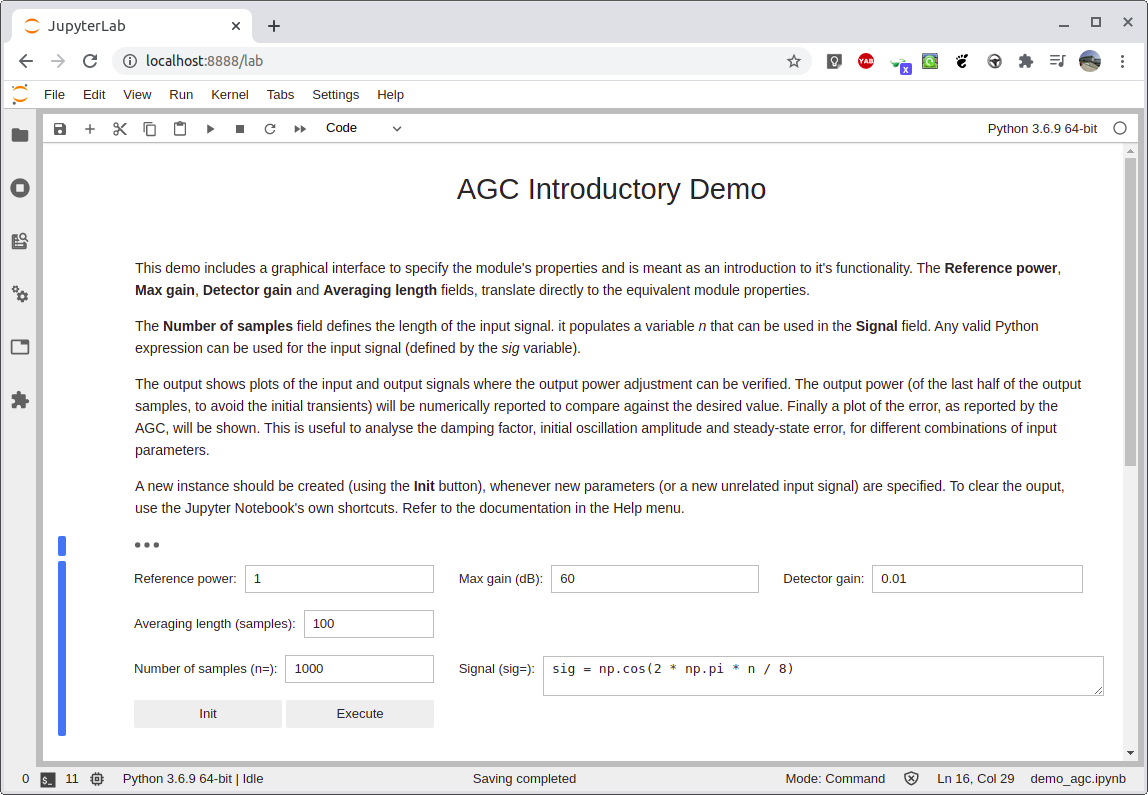
\includegraphics[width=0.75\textwidth]{demo_agc_interface}
  \caption{\code{AGC} Jupyter notebook demonstration interface}
  \label{fig:demo_agc_interface}
\end{figure}

\begin{figure}[H]
  \centering
  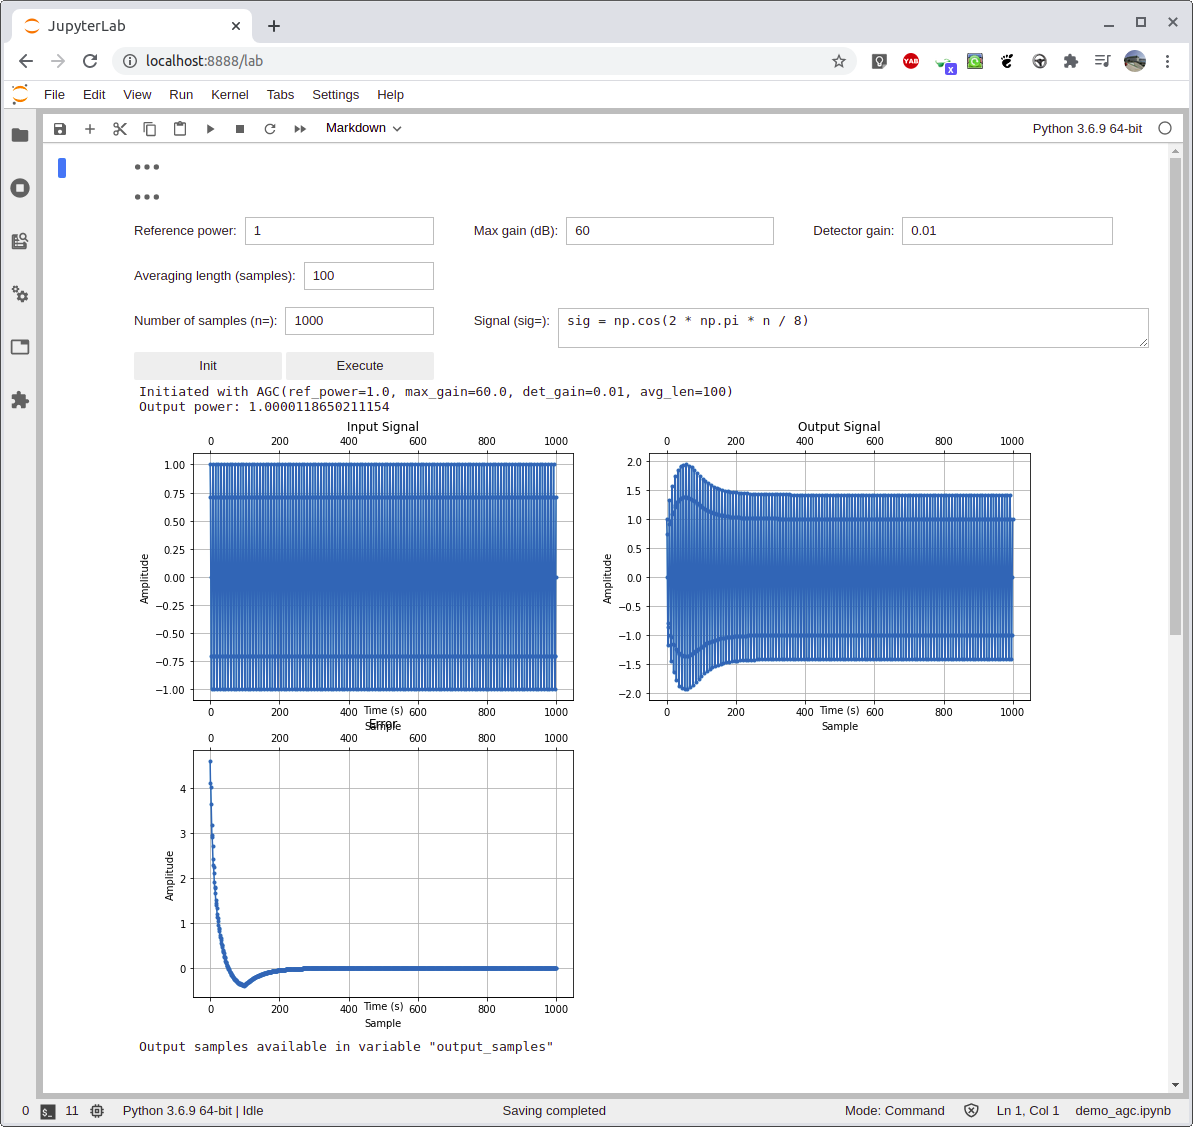
\includegraphics[width=0.75\textwidth]{demo_agc}
  \caption{\code{AGC} Jupyter notebook demonstration results}
  \label{fig:demo_agc}
\end{figure}

%%%%%%%%%%%%%%%%%%%%%%%%%%%%%%%%%%%%%%%%%%%%%%%%%%%%%%%%%%%%%%%%%%%%%%%%%%%%%%%
\section{Phase Ambiguity Correction}

As mentioned in \autoref{sect:library_freq_sync} and seen in the S-curves from \autoref{fig:s_curve_qpsk} and \autoref{fig:s_curve_bpsk}, the phase detector algorithm can lock onto a phase that $\pm 180\degree$ from the correct phase (for BPSK) and $[\pm 90\degree,\pm 180\degree,\pm 270\degree]$ for QPSK. This module resolves this ambiguity.

\noindent Module properties:
\begin{itemize}
  \item \code{preamble}: The modulated preamble, as sent by the transmitter
\end{itemize}

The module takes a known sequence, like a preamble, and compares the phase of this sequence with the phase of the same sequence embedded in the input signal (which could have an erroneous phase offset). The algorithm can be described as follows:
\begin{itemize}
  \item The input signal is expressed as $x(n) = p(n)e^{j\phi} + w(n)$, where $p(n)$ is the preamble, $\phi$ is the phase to be estimated and $w(n)$ is a noise term.
  \item Compute $y_1(t) = p^*(n)x(n) = e^{j\phi} + x^*(n)w(n)$, where $*$ denotes complex conjugation.
  \item The goal is to estimate the value $\phi$ from the observation $y_1(n)$, i.e., estimate the value $B = e^{j\phi}$, and $\phi = \text{angle}(B)$. Suppose $w(n)$ yields a i.i.d. complex AWGN distribution $\mathcal{N}(0,\sigma^2)$. Then a non-biased estimator could be $\hat{B} = \frac{1}{N}\sum_{n=0}^{N-1} y_1(n)$, where $N$ is the number of samples in the preamble. In that case $\hat\phi = \text{angle}(\hat{B})$ and the variance of the estimator $\hat{B}$ is $\frac{\sigma^2}{N}$.
  \item Once $\phi$ has been estimated, remove it from the input signal. The output signal becomes $y(n) = x(n)e^{-j\phi}$.
\end{itemize}

%%%%%%%%%%%%%%%%%%%%%%%%%%%%%%%%%%%%%%%%%%%%%%%%%%%%%%%%%%%%%%%%%%%%%%%%%%%%%%%
\section{Channel Models and Impairments}
This sections describes the channel models and impairments available in the SKSDR library.

\subsection{AWGN Channel}

The \code{AWGNChannel} class implements a simple \emph{additive white Gaussian channel noise} model.

\noindent Module properties:
\begin{itemize}
  \item \code{snr}: The desired SNR
  \item \code{signal\_power}: The expected signal power, or `measured' if the power is to measured dynamically each time the module is invoked.
\end{itemize}

The algorithm draws the noise as values from the standard normal distribution, scaled to the appropriate power in order to fulfil the desired SNR (specified by the \code{snr} property). It then returns the input signal added to this generated noise.

\subsection{Phase/Frequency Impairment}
The \code{PhaseFrequencyOffset} module applies phase and frequency offsets to an incoming signal.

\noindent Module properties:
\begin{itemize}
  \item \code{sample\_rate} (Hz): The input signal sample rate
  \item \code{freq\_offset} (Hz): The desired frequency offset
  \item \code{phase\_offset} (degrees): The desired phase offset
\end{itemize}

The phase offset parameter (specified by \code{phase\_offset}) adds a constant to the phase of the signal. The frequency offset parameter (specified by \code{freq\_offset}) determines the rate of change of the signal's phase. If one sets the frequency offset to a positive number, the symbol points on a scatter plot, will fall on a rotating grid, corresponding to the standard constellation, which revolves at a constant rate in the counter-clockwise direction.

Given an input sequence $x(n)$, the module computes
\begin{align}
  y(n) = x(n)e^{j(\omega nT + \phi)}
\end{align}
where $\omega$ is the frequency offset, $T$ is the sampling period and $\phi$ is the phase offset.

\autoref{lst:demo_phase_freq_offset} shows a demo of this module, using IPython. A phase offset of 30° and a frequency offset of 1\% of the sample rate are introduced in a QPSK signal. The original signal and signals with offsets are plotted for comparison. \autoref{fig:demo_phase_freq_offset} shows the resulting scatter plots.

\begin{python}[label={lst:demo_phase_freq_offset},caption={\code{PhaseFrequencyOffset} demo}]
  In [1]: import matplotlib.gridspec as gridspec
  ...: import matplotlib.pyplot as plt
  ...: import numpy as np
  ...:
  ...: import sksdr
  ...:
  ...: # Create a phase and frequency offset object, where the phase offset is 30 degrees
  ...: pfo_phase = sksdr.PhaseFrequencyOffset(phase_offset=30, sample_rate=1e6)
  ...:
  ...: # Create a phase and frequency offset object, where the frequency offset is
  ...: # 1 percent of the sample rate
  ...: pfo_freq = sksdr.PhaseFrequencyOffset(freq_offset=1e4, sample_rate=1e6)
  ...:
  ...: # Generate random data symbols and apply QPSK modulation
  ...: ints = np.random.randint(0, 4, 1000)
  ...: bits = sksdr.x2binlist(ints, 2)
  ...: psk = sksdr.PSKModulator(sksdr.QPSK, [0, 1, 3, 2], 1.0, np.pi/4)
  ...: mod_sig = psk.modulate(bits)
  ...:
  ...: # Apply phase and frequency offsets
  ...: mod_sig_phase_off, _ = pfo_phase(mod_sig)
  ...: mod_sig_freq_off, _ = pfo_freq(mod_sig)
  ...:
  ...: # Setup figure
  ...: fig = plt.figure(figsize=(15,10))
  ...: gs = gridspec.GridSpec(2, 2, figure=fig)
  ...:
  ...: # Scatter plot of the original signal
  ...: f = sksdr.scatter_plot(mod_sig, 'Original Signal', fig=fig, gs=gs[0, 0])
  ...:
  ...: # Scatter plot of the signal with phase offset
  ...: f = sksdr.scatter_plot(mod_sig_phase_off,
  ...:                        'Signal with phase offset of 30 degrees',
  ...:                        fig=fig, gs=gs[1, 0])
  ...:
  ...: # Scatter plot of the signal with frequency offset
  ...: f = sksdr.scatter_plot(mod_sig_freq_off,
  ...:                       'Signal with frequency offset of 1 percent of sample rate',
  ...:                       fig=fig, gs=gs[1, 1])
  ...:
  ...: f.show()
\end{python}

\begin{figure}[H]
  \centering
  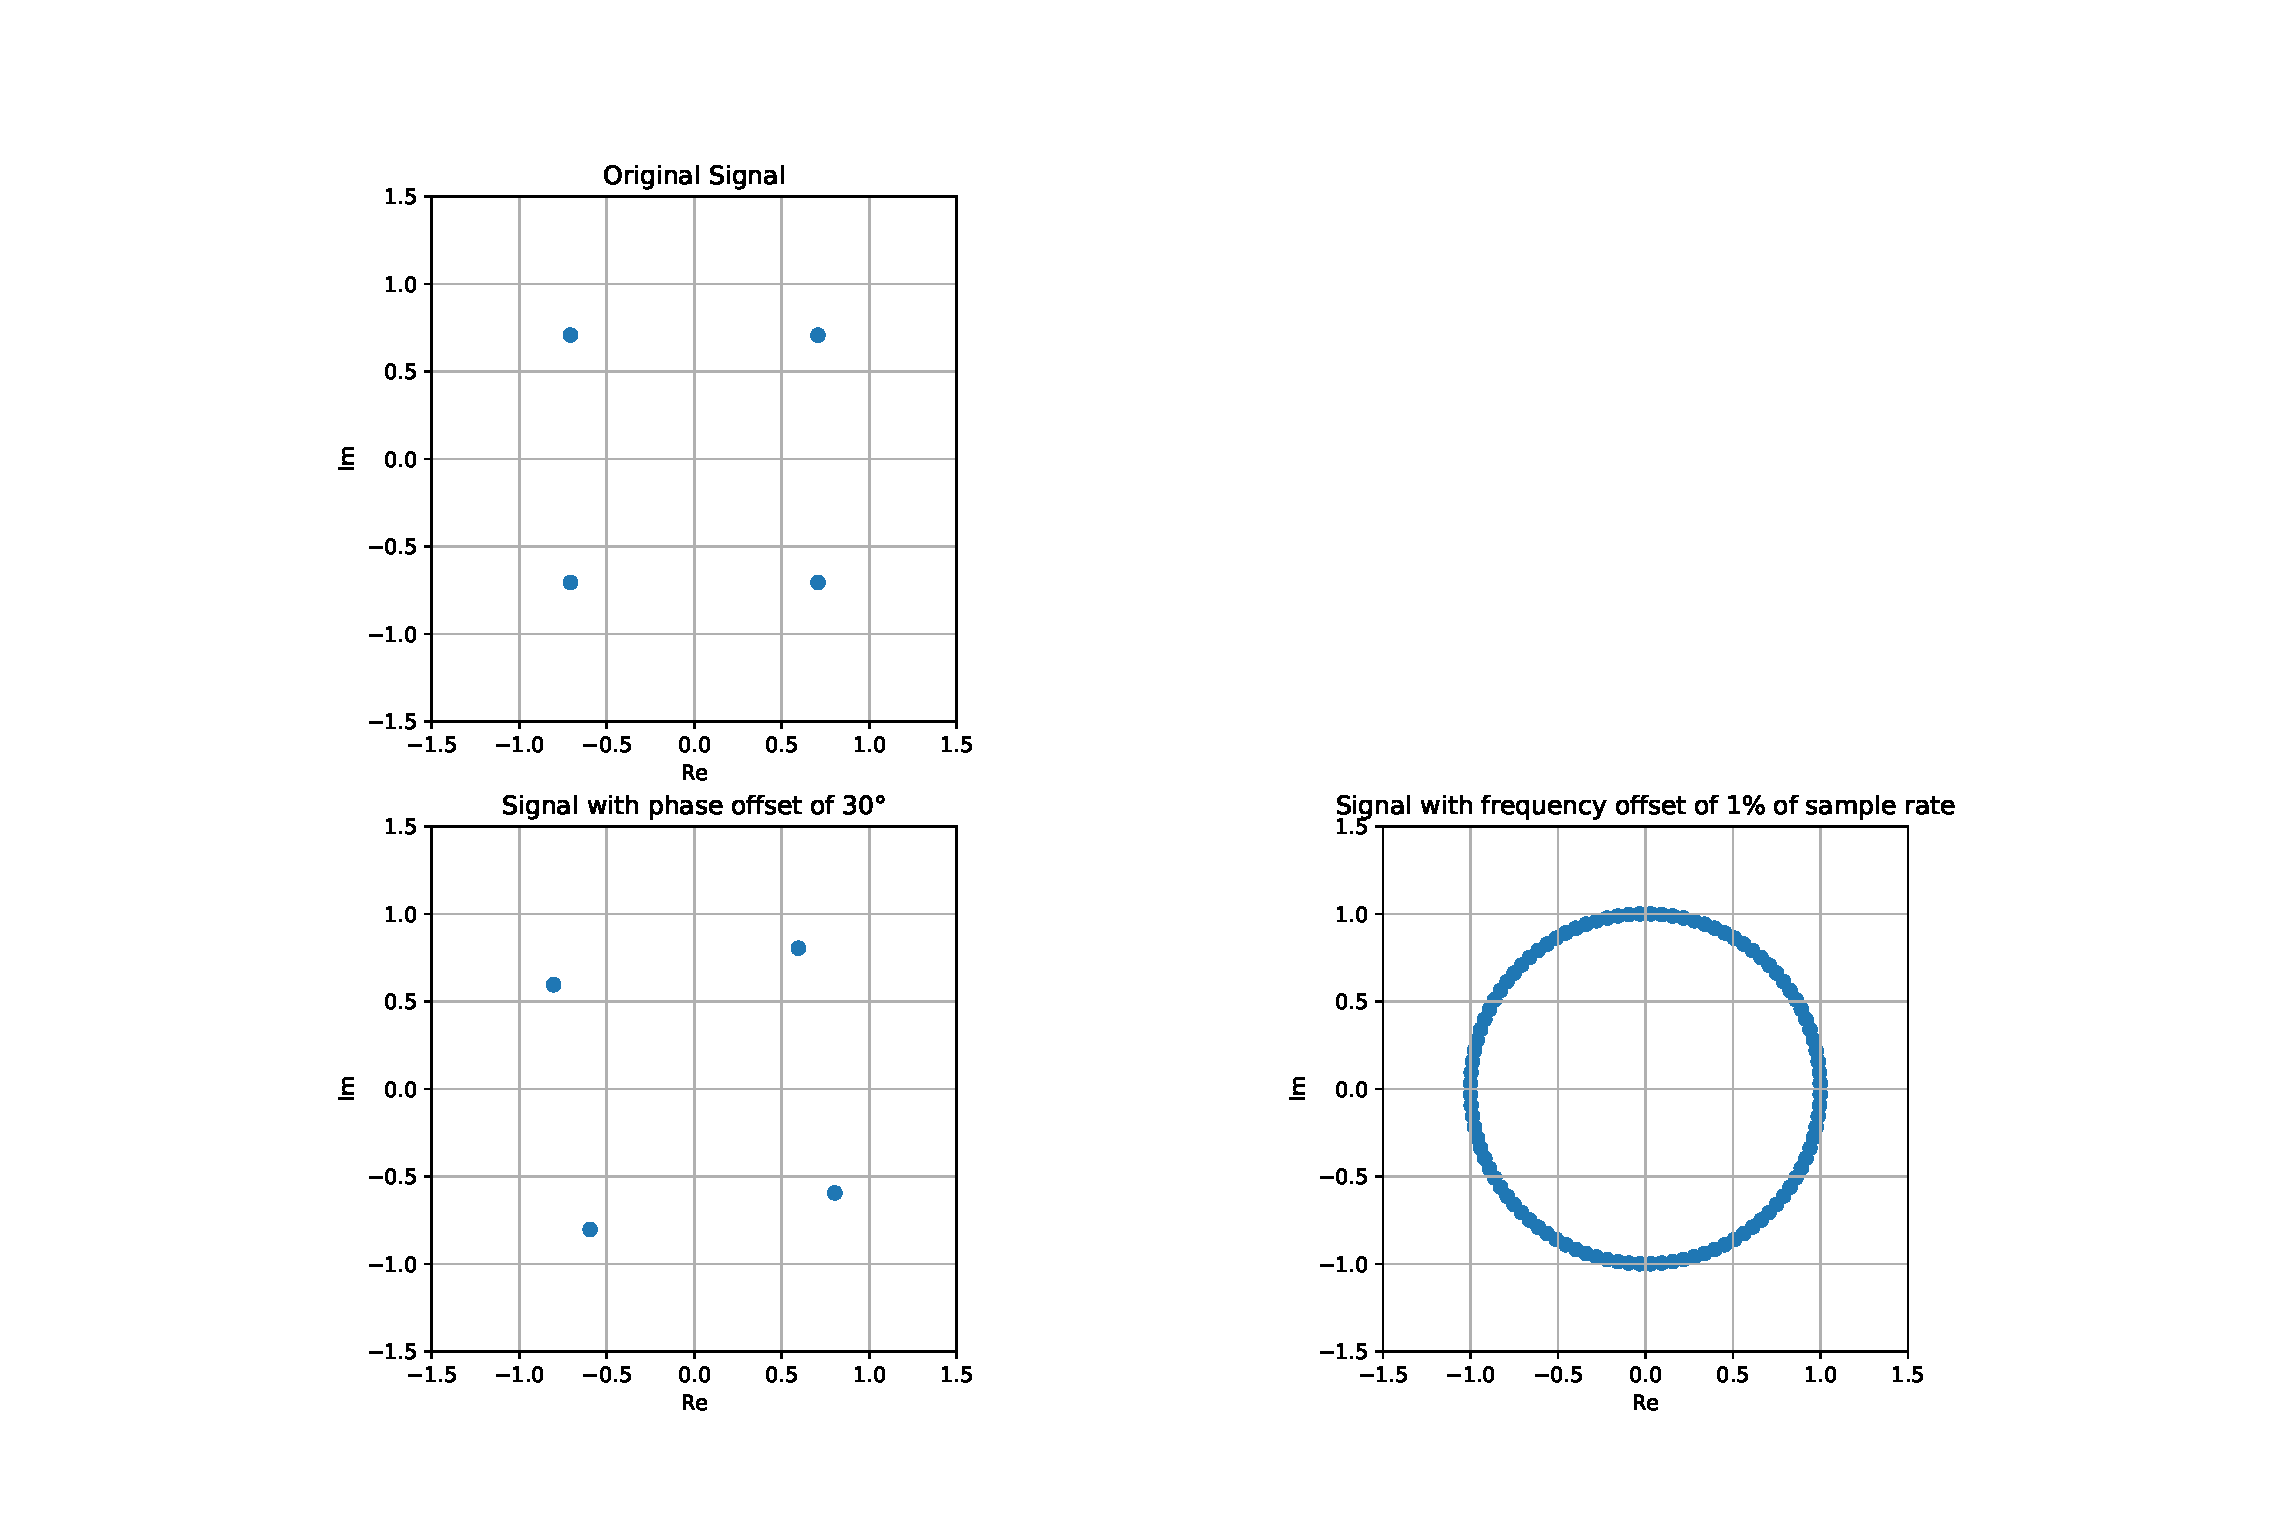
\includegraphics[width=\textwidth]{demo_phase_freq_offset}
  \caption{\code{PhaseFrequencyOffset} demo scatter plots of the original signal and signals with 30° phase offset and 1\% of sample rate frequency offset}
  \label{fig:demo_phase_freq_offset}
\end{figure}

\subsection{Delay Impairment}

The \code{VariableFractionalDelay} module delays the input signal by a specified (and potentially fractional) number of samples.

\noindent Module properties:
\begin{itemize}
  \item \code{max\_delay} (samples): The maximum delay
  \item \code{init\_state}: The initial value to fill in the circular buffer that holds the samples (default=0).
\end{itemize}

The module interpolates the input signal to obtain new samples at non-integer sampling intervals. The only available interpolation method currently is \emph{linear} interpolation. The delay can vary with each invocation of the module (specified by the \code{delay} argument in the \code{\_\_call\_\_()} function). This allows to create a delay profile say, for example, in a triangle or sawtooth shape. The maximum value of the delay is specified using \code{max\_delay}. Delay values greater than the maximum are clipped to the maximum.

The module has a circular buffer of size $\code{max\_delay}+1$ that holds the previous samples, from which it can then compute the interpolation, to obtain the output sequence.

\autoref{lst:demo_delay_offset} shows a demo of this module, using IPython. A QPSK signal is delayed by 1 sample and both the original and delayed signals are plotted for comparison. \autoref{fig:demo_delay_offset} shows the resulting plot. Note in this case the delay offset is fixed to 1 sample, but in general, it can vary in each call to the module.

\begin{python}[label={lst:demo_delay_offset},caption={\code{VariableFractionalDelay} demo}]
  In [17]: import matplotlib.pyplot as plt
    ...: import numpy as np
    ...:
    ...: import sksdr
    ...:
    ...: # Create a delay offset object
    ...: vfd = sksdr.VariableFractionalDelay(max_delay=2)
    ...:
    ...: # Generate random data symbols and apply QPSK modulation
    ...: ints = np.random.randint(0, 4, 10000)
    ...: bits = sksdr.x2binlist(ints, 2)
    ...: psk = sksdr.PSKModulator(sksdr.QPSK, [0, 1, 3, 2], 1.0, np.pi/4)
    ...: mod_sig = psk.modulate(bits)
    ...:
    ...: # Interpolate by 4 and filter with RRC tx filter
    ...: interp = sksdr.FirInterpolator(4, sksdr.rrc(4, 0.5, 10))
    ...: _, tx_sig = interp(mod_sig)
    ...:
    ...: # Apply a delay offset of 1 sample
    ...: tx_sig_off = vfd(tx_sig, 1)
    ...:
    ...: plt.plot(tx_sig.real[:100], '.-', label='Original signal')
    ...: plt.plot(tx_sig_off.real[:100], '.-', label='Delayed signal (1 sample)')
    ...: plt.title('Delayed signal impairment demo')
    ...: plt.grid()
    ...: plt.legend()
    ...: plt.show()
\end{python}

\begin{figure}[H]
  \centering
  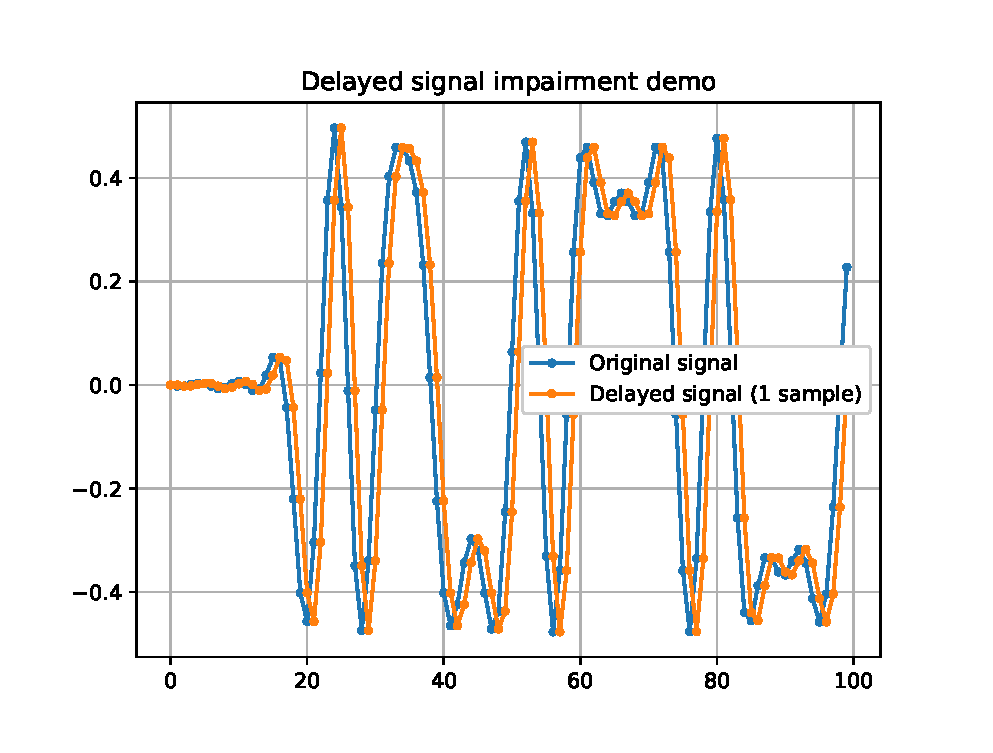
\includegraphics[width=0.75\textwidth]{demo_delay_offset}
  \caption{\code{VariableFractionalDelay} demo plot of the original signal and the delayed signal}
  \label{fig:demo_delay_offset}
\end{figure}

%%%%%%%%%%%%%%%%%%%%%%%%%%%%%%%%%%%%%%%%%%%%%%%%%%%%%%%%%%%%%%%%%%%%%%%%%%%%%%%
\section{Scrambling/Descrambling}

\subsection{Scrambler}

The \code{Scrambler} module scrambles an input signal using a \emph{linear feedback shift register} (LFSR).

\noindent Module properties:
\begin{itemize}
  \item \code{poly}: On/off state for each switch
  \item \code{init\_state}: Initial values of the registers
\end{itemize}

Scrambling is necessary to ensure a signal doesn't contain long sequences of 0's or 1's, which can jeopardize the performance of various blocks, such as the ZCTED discussed in \autoref{sect:timing_error_detector}. \autoref{fig:scrambler_diagram} shows the operation of the Scrambler.

\begin{figure}
\centering
\begin{tikzpicture} [circuit ee IEC,
                     small circuit symbols,
                     every info/.style={font=\footnotesize},
                     set make contact graphic= var make contact IEC graphic,]

\matrix (m1) [row sep=10mm, column sep=10mm]
{
  %--------------------------------------------------------------------
  \node[coordinate] (m00) {}; &
  \node[coordinate] (m01) {}; &
  \node[dspnodeopen,dsp/label=above] (m02) {$y(n)$}; \\
  %--------------------------------------------------------------------
  \node[dspnodeopen,dsp/label=above] (m10) {$x(n)$}; &
  \node[dspadder] (m11) {}; &
  \node[dspsquare] (m12) {1}; &
  \node[dspsquare] (m13) {2}; &
  \node[coordinate] (m14) {}; &
  \node[coordinate] (m15) {}; &
  \node[dspsquare, inner xsep=1mm] (m16) {$M-1$}; &
  \node[dspsquare] (m17) {$M$}; \\
  %--------------------------------------------------------------------
  \node[coordinate] (m20) {}; &
  \node[coordinate] (m21) {}; &
  \node[coordinate] (m22) {}; &
  \node[coordinate] (m23) {}; &
  \node[coordinate] (m24) {}; &
  \node[coordinate] (m25) {}; &
  \node[coordinate] (m26) {}; &
  \node[coordinate] (m27) {}; \\
  %--------------------------------------------------------------------
  \node[coordinate] (m30) {}; &
  \node[coordinate] (m31) {}; &
  \node[dspadder] (m32) {}; &
  \node[dspadder] (m33) {}; &
  \node[coordinate] (m34) {}; &
  \node[coordinate] (m35) {}; &
  \node[dspadder] (m36) {}; &
  \node[coordinate] (m37) {}; \\
};

% Draw connections

\begin{scope}[start chain]
  \chainin (m10);
  \chainin (m11) [join=by dspconn];
  \chainin (m12) [join=by dspconn];
  \chainin (m13) [join=by dspconn];
  \chainin (m14) [join=by dspconn];
  \chainin (m15) [join=by dashed];
  \chainin (m16) [join=by dspconn];
  \chainin (m17) [join=by dspconn];
\end{scope}

\begin{scope}[start chain]
  \chainin (m11);
  \chainin (m01) [join=by dspline];
  \chainin (m02) [join=by dspconn];
\end{scope}

\begin{scope}[start chain]
  \chainin (m37) [join=by dspline];
  \chainin (m36) [join=by dspconn];
  \chainin (m35) [join=by dspconn];
  \chainin (m34) [join=by dashed];
  \chainin (m33) [join=by dspconn];
  \chainin (m32) [join=by dspconn];
  \chainin (m31) [join=by dspline];
  \chainin (m11) [join=by dspconn];
\end{scope}

\draw (m12) to[make contact={near end,info'={$p_1$}}] (m22);
\draw[dspconn] (m22) to (m32);
\draw (m13) to[make contact={near end,info'={$p_2$}}] (m23);
\draw[dspconn] (m23) to (m33);
\draw (m16) to[make contact={near end,info'={$p_{m-1}$}}] (m26);
\draw[dspconn] (m26) to (m36);
\draw (m17) to[make contact={near end,info'={$p_m$}}] (m27);
\draw[dspline] (m27) to (m37);

\end{tikzpicture}
\caption{Scrambler block diagram}
\label{fig:scrambler_diagram}
\end{figure}

At each time step, the input causes the contents of the registers to shift sequentially. Notice that the output for a particular bit depends solely on the $M$ previous bits (excluding the first $N$ bits that will also depend on the initial conditions, where $N$ is the size of the shift register).

\subsection{Descrambler}

The \code{Descrambler} module is used to retrieve the original bit sequence, given an input sequence that's been scrambled using the \code{Scrambler} module.

\noindent Module properties:
\begin{itemize}
  \item \code{poly}: On/off states of the switches
  \item \code{init\_state}: Initial values of the registers
\end{itemize}

\autoref{fig:descrambler_diagram} shows the operation of the Descrambler.

\begin{figure}
\centering
\begin{tikzpicture} [circuit ee IEC,
                     small circuit symbols,
                     every info/.style={font=\footnotesize},
                     set make contact graphic= var make contact IEC graphic,]

\matrix (m1) [row sep=10mm, column sep=10mm]
{
  %--------------------------------------------------------------------
  \node[dspnodeopen,dsp/label=above] (m00) {$x(n)$}; &
  \node[dspnodefull] (m01) {}; &
  \node[dspsquare] (m02) {1}; &
  \node[dspsquare] (m03) {2}; &
  \node[coordinate] (m04) {}; &
  \node[coordinate] (m05) {}; &
  \node[dspsquare, inner xsep=1mm] (m06) {$M-1$}; &
  \node[dspsquare] (m07) {$M$}; \\
  %--------------------------------------------------------------------
  \node[coordinate] (m10) {}; &
  \node[coordinate] (m11) {}; &
  \node[coordinate] (m12) {}; &
  \node[coordinate] (m13) {}; &
  \node[coordinate] (m14) {}; &
  \node[coordinate] (m15) {}; &
  \node[coordinate] (m16) {}; &
  \node[coordinate] (m17) {}; \\
  %--------------------------------------------------------------------
  \node[coordinate] (m20) {}; &
  \node[dspadder,label={above right:$+$},label={below right:$-$}] (m21) {}; &
  \node[dspadder] (m22) {}; &
  \node[dspadder] (m23) {}; &
  \node[coordinate] (m24) {}; &
  \node[coordinate] (m25) {}; &
  \node[dspadder] (m26) {}; &
  \node[coordinate] (m27) {}; \\
  %--------------------------------------------------------------------
  \node[coordinate] (m30) {}; &
  \node[coordinate] (m31) {}; &
  \node[dspnodeopen,dsp/label=above] (m32) {$y(n)$}; \\
};

% Draw connections

 \begin{scope}[start chain]
  \chainin (m00);
  \chainin (m01) [join=by dspline];
  \chainin (m02) [join=by dspconn];
  \chainin (m03) [join=by dspconn];
  \chainin (m04) [join=by dspconn];
  \chainin (m05) [join=by dashed];
  \chainin (m06) [join=by dspconn];
  \chainin (m07) [join=by dspconn];
\end{scope}

\begin{scope}[start chain]
  \chainin (m01);
  \chainin (m21) [join=by dspconn];
  \chainin (m31) [join=by dspline];
  \chainin (m32) [join=by dspconn];
\end{scope}

\begin{scope}[start chain]
  \chainin (m27) [join=by dspline];
  \chainin (m26) [join=by dspconn];
  \chainin (m25) [join=by dspconn];
  \chainin (m24) [join=by dashed];
  \chainin (m23) [join=by dspconn];
  \chainin (m22) [join=by dspconn];
  \chainin (m21) [join=by dspconn];
\end{scope}

\draw (m02) to[make contact={near end,info'={$p_1$}}] (m12);
\draw[dspconn] (m12) to (m22);
\draw (m03) to[make contact={near end,info'={$p_2$}}] (m13);
\draw[dspconn] (m13) to (m23);
\draw (m06) to[make contact={near end,info'={$p_{m-1}$}}] (m16);
\draw[dspconn] (m16) to (m26);
\draw (m07) to[make contact={near end,info'={$p_m$}}] (m17);
\draw[dspline] (m17) to (m27);

\end{tikzpicture}
\caption{Descrambler block diagram}
\label{fig:descrambler_diagram}
\end{figure}

At each time step, the input causes the contents of the registers to shift sequentially. Similarly to the Scramber, the output for a particular bit depends solely on the $M$ previous bits (excluding the first $N$ bits that will also depend on the initial conditions, where $N$ is the size of the shift register).

In both modules, the \code{init\_state} list size must be equal to the \code{poly} list size - 1. The Descrambler \code{poly} and \code{init\_state} must be the same as the ones used in the corresponding Scrambler.

\subsection{Example}

\autoref{lst:scrambling_example} shows an application example of this module, using the IPython console. A stream of bits is scrambler and then descrambled. The descrambled bit sequence is identical to the input bit sequence.
\begin{python}[label={lst:scrambling_example},caption={Scrambling and Descrambling example}]
  In [4]: import sksdr
  ...: scrambler = sksdr.Scrambler([1, 0, 1, 1, 0], [0,1,1,])
  ...: descrambler = sksdr.Descrambler([1, 0, 1, 1, 0], [0,1,1,])
  ...: print('Initiated scrambler with ' + repr(scrambler))
  ...: in_bits = np.random.randint(0, 2, 100)
  ...: scrambled_bits = scrambler(in_bits)
  ...: descrambled_bits = descrambler(scrambled_bits)
  ...: print('Original bits: ' + repr(in_bits))
  ...: print('Scrambled bits: ' + repr(scrambled_bits))
  ...: print('Descrambled bits: ' + repr(descrambled_bits))
Initiated scrambler with Scrambler(poly=[1, 0, 1, 1, 0], init_state=[0, 1, 1])
Original bits: array([
      0, 1, 1, 1, 1, 1, 1, 0, 0, 0, 0, 1, 1, 0, 0, 0, 0, 1, 0, 0, 1, 0,
      1, 0, 0, 1, 0, 0, 0, 0, 0, 1, 1, 0, 1, 1, 0, 1, 0, 1, 1, 0, 0, 0,
      1, 0, 1, 1, 0, 1, 0, 1, 0, 0, 1, 1, 1, 0, 1, 1, 0, 1, 0, 0, 0, 1,
      1, 0, 0, 0, 0, 1, 1, 0, 1, 0, 0, 0, 1, 1, 0, 0, 0, 1, 0, 0, 0, 1,
      0, 1, 0, 1, 1, 0, 0, 0, 1, 0, 0, 1])
Scrambled bits: array([
      0, 0, 1, 1, 0, 1, 0, 1, 1, 1, 0, 1, 0, 1, 1, 1, 0, 1, 1, 1, 1, 0,
      1, 1, 1, 1, 0, 0, 1, 0, 1, 0, 0, 1, 1, 0, 0, 0, 0, 1, 1, 1, 0, 0,
      0, 0, 1, 1, 1, 1, 0, 1, 1, 1, 1, 1, 1, 0, 1, 0, 1, 0, 1, 1, 1, 1,
      1, 0, 0, 1, 0, 0, 0, 0, 1, 0, 1, 1, 0, 1, 1, 1, 0, 1, 1, 1, 0, 1,
      1, 0, 0, 0, 1, 0, 1, 1, 0, 0, 1, 1])
Descrambled bits: array([
      0, 1, 1, 1, 1, 1, 1, 0, 0, 0, 0, 1, 1, 0, 0, 0, 0, 1, 0, 0, 1, 0,
      1, 0, 0, 1, 0, 0, 0, 0, 0, 1, 1, 0, 1, 1, 0, 1, 0, 1, 1, 0, 0, 0,
      1, 0, 1, 1, 0, 1, 0, 1, 0, 0, 1, 1, 1, 0, 1, 1, 0, 1, 0, 0, 0, 1,
      1, 0, 0, 0, 0, 1, 1, 0, 1, 0, 0, 0, 1, 1, 0, 0, 0, 1, 0, 0, 0, 1,
      0, 1, 0, 1, 1, 0, 0, 0, 1, 0, 0, 1])
\end{python}

%%%%%%%%%%%%%%%%%%%%%%%%%%%%%%%%%%%%%%%%%%%%%%%%%%%%%%%%%%%%%%%%%%%%%%%%%%%%%%%
\section{Forward Error Correcting Algorithms}
Forward error correction (FEC) is a technique used for detecting and possibly correcting errors in data transmission over unreliable communication channels \cite{wikipedia_fec}. This is achieved by adding redundant information to the message, that is then used by the receiver in the error detection process. FEC allows the receiver correct errors without needing to request re-transmission of data, but at the cost of a higher channel bandwidth. This is specially useful for systems in which re-transmissions are not viable due to latency issues for example.
The maximum proportion of errors or missing bits that can be corrected is determined by the design of the ECC, so different forward error correcting codes are suitable for different conditions.

\subsection{Hamming(7,4) Code}

The Hamming(7,4) was developed in the SKSDR library as way of demonstration and experimentation. The idea is that the library can be extended in the future with other algorithms including for example convolutional codes like Viterbi coding.

\noindent Module properties:
\begin{itemize}
  \item \code{ntotal}: The total number of bits (data + parity) (currently fixed as 7)
  \item \code{ndata}: The number of data bits (currently fixed as 4)
\end{itemize}

Hamming(7,4) is a linear error-correcting code that encodes four bits of data into seven bits by adding three parity bits \cite{wikipedia_hamming}. The algorithm can correct any single-bit error, or detect all single-bit and two-bit errors. Because Hamming codes are linear codes, they can be computed efficiently using matrices. Two Hamming matrices can be defined, the code \emph{generator matrix} G and the \emph{parity-check matrix} H:
\begin{equation}
\mathbf{G^T} := \begin{pmatrix}
  1 & 1 & 0 & 1 \\
  1 & 0 & 1 & 1 \\
  1 & 0 & 0 & 0 \\
  0 & 1 & 1 & 1 \\
  0 & 1 & 0 & 0 \\
  0 & 0 & 1 & 0 \\
  0 & 0 & 0 & 1 \\
 \end{pmatrix}, \qquad \mathbf{H} := \begin{pmatrix}
  1 & 0 & 1 & 0 & 1 & 0 & 1 \\
  0 & 1 & 1 & 0 & 0 & 1 & 1 \\
  0 & 0 & 0 & 1 & 1 & 1 & 1 \\
 \end{pmatrix}.
\end{equation}

One can be derived from the other. For example, if the generator matrix for an [n,k]-code is in standard form:
\begin{equation}
  G = \begin{bmatrix} I_k | P \end{bmatrix}
\end{equation}
then the parity check matrix is given by
\begin{equation}
  H = \begin{bmatrix} -P^{\top} | I_{n-k} \end{bmatrix}
\end{equation}
because
\begin{equation}
G H^{\top} = P-P = 0
\end{equation}

\autoref{fig:hamming_74} illustrates the relationship between the data bits and the parity bits, showing which data bits are covered by each of the parity bits.

\begin{figure}[H]
  \centering
  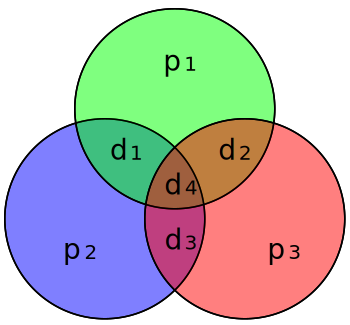
\includegraphics[width=0.25\textwidth]{hamming_74}
  \caption{Venn diagram showing the relationship between data bits and parity bits in the Hamming(7,4) code [\citeauthor{image:hamming74_venn_diagram}]}
  \label{fig:hamming_74}
\end{figure}

\autoref{lst:hamming_74} shows an application example of this module, using the IPython console. A stream of bits is encoded and an error is introduced in one bit. The stream is then decoded and the error is corrected. The output bit sequence is identical to the input bit sequence.

\begin{python}[label={lst:hamming_74},caption={Hamming(7,4) example}]
In [46]: import sksdr
  ...: h74 = sksdr.Hamming(7, 4)
  ...: msg = [1, 0, 0, 1]
  ...: send = h74.encode(msg)
  ...: # Introduce an error by inverting one of the data or parity bits
  ...: send[2] = send[2] ^ 1
  ...: recv = h74.decode(send)
  ...: recv
  ...:
Out[46]: (array([1, 0, 0, 1]), array([2]))
\end{python}


\chapter{Demonstration Applications}
\label{chap:demo_apps}
This chapter presents the development process and details of the chosen GNU Radio applications for this thesis. \autoref{sect:gnu_radio_hack_rf_one_rtl_sdr_overview} provides an introduction to GNU Radio platform and application development, and the hardware later used for real-time testing (the HackRF One and the RTL-SDR). The following sections describe the two applications. The first, a WBFM Receiver, is intended as an introduction to developing SDR applications in GNU Radio and to demonstrate the potential for SDR to easily replace legacy analogue systems. The second, a PSK transceiver, will make full use of the SKSDR library and is intended to demonstrate application of several DSP blocks needed for digital communication systems.

%%%%%%%%%%%%%%%%%%%%%%%%%%%%%%%%%%%%%%%%%%%%%%%%%%%%%%%%%%%%%%%%%%%%%%%%%%%%%%%
\section{GNU Radio, HackRF One and RTL-SDR Overview}
\label{sect:gnu_radio_hack_rf_one_rtl_sdr_overview}

As previously mentioned, the hardware supporting this thesis is a HackRF One and an RTL-SDR. The HackRF One (shown in \autoref{fig:hackrf_one_detail}) is based on an analogue quadrature system, similar to the one described in \autoref{sect:analogue_quadrature_receiver_architecture}. The IF frequency is tuneable and is in 2.4 GHz industrial, scientific and medica (ISM) band. A high IF allows for a fairly relaxed image rejection filter. At the same time, it's relatively affordable to source IF mixer and VCO ICs designed to operate in the ISM bands. For critical phase noise and frequency stability (for example GPS applications) it's possible to install an external temperature compensated crystal oscillator (TCXO), which provide down to 0.5 ppm accuracy. Given the open hardware nature of this device, quite a few clones exist on the market. For this project, due to budget restrictions, a device sourced by Banggood was selected (specifically \href{https://pt.banggood.com/HackRF-One-1MHz-6GHz-Radio-Platform-Development-Board-Software-Defined-RTL-SDR-Demoboard-Kit-Dongle-Receiver-Ham-Radio-p-1552853.html}{this one})

\begin{figure} [ht]
  \begin{subfigure}{.5\textwidth}
    \centering
    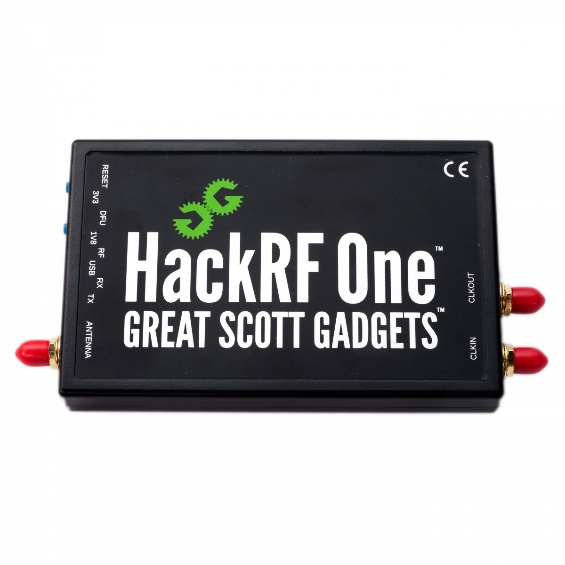
\includegraphics[width=.8\linewidth]{hack_rf_one}
    \label{fig:hackrf_one_case}
  \end{subfigure}
  \begin{subfigure}{.5\textwidth}
    \centering
    \includegraphics[width=.8\linewidth]{hackrf_block_diagram}
    \label{fig:hackrf_one_block_diagram}
  \end{subfigure}
  \caption[The HackRF One case and block diagram]{The HackRF One comes with a brushed aluminium case and has 3 SMA ports (RF, Clock In and Clock Out). It has a 30 MHz to 6 GHz frequency range and 20 MHz bandwidth with 8 bits resolution [\citeauthor{hackrf_one_product}].}
  \label{fig:hackrf_one_detail}
\end{figure}

The RTL-SDR's original function is a DVB-T receiver but it was discovered by the community that it actually allows direct access to the IQ samples (in addition to the fully decoded MPEG signal which is its original application). This `undocumented' interface, however, has a limited bandwidth of 3.2 MHz. \autoref{fig:rtlsdr_detail} shows the physical format of the RTL-SDR USB dongle and a block diagram of its architecture. The device is based on a two-chip solution. An RF front-end (the R820T tuner IC) and the baseband IC composed of an ADC, video decoding and USB streaming logic. Note this IC is protected by non-disclosure agreement (NDA) so there is limited available knowledge about it.

\begin{figure} [ht]
  \begin{subfigure}{.5\textwidth}
    \centering
    \includegraphics[width=.6\linewidth]{rtlsdr_case}
    \label{fig:rtlsdr_case}
  \end{subfigure}
  \begin{subfigure}{.5\textwidth}
    \centering
    \includegraphics[width=1\linewidth]{rtlsdr_block_diagram}
    \label{fig:rtlsdr_block_diagram}
  \end{subfigure}
  \caption{The RTL-SDR USB dongle and the high-level block diagram, based on a two-chip solution [\citeauthor{rtlsdr_product}]}
  \label{fig:rtlsdr_detail}
\end{figure}

The applications are developed using the GNU Radio framework. GNU Radio is a free software development toolkit that provides signal processing blocks to implement software-defined radios and signal processing systems \cite{gnuradio_project}. It can be used with external RF hardware to create software-defined radios, or without hardware in a simulation-like environment. The GNU Radio applications consist of \emph{flowgraphs}, which are a series of connected signal processing blocks, thus describing a signal flow. The GNU Radio infrastructure is written entirely in C++, and many of the user tools are written in Python. Its graphical interface is supported by the Qt library (which as bindings for several languages such as Python through PyQt) and the wxWidgets library (considered deprecated for GNU Radio development, so its use is discouraged). GNU Radio runs mostly in GPP-based hardware although there are ongoing efforts to adapt the framework for FPGA and GPU-based platforms \cite{gr2020_program}.
\autoref{fig:simple_gr_demo} shows a very simple example of a flowgraph where one can see several types of blocks, like \emph{Source} and \emph{Sink}. Also, \emph{Variable} and \emph{Options} blocks, which allow for a more flexible workflow. Note that it's possible to use Python expressions and variables in most blocks input fields. The \emph{Throttle} block is usually used when there is no hardware limiting the sample rate, and its purpose is to prevent GNU Radio consuming samples as fast as possible, thereby consuming all the CPU time. In \autoref{fig:simple_gr_demo_exec} the \emph{Time Sink} interface is displayed, when the flowgraph is running. The frequency can be changed in real-time.

\begin{figure}[H]
  \centering
  \includegraphics[width=0.75\textwidth]{simple_gr_demo}
  \caption[Simple GNU Radio flowgraph consisting of an input signal with added AWGN noise]{Simple GNU Radio flowgraph consisting of an input signal with added AWGN noise. The input signal with and without noise is visualized in a two \emph{Time Sink} blocks.}
  \label{fig:simple_gr_demo}
\end{figure}

\begin{figure}[H]
  \centering
  \includegraphics[width=0.75\textwidth]{simple_gr_demo_exec}
  \caption[Execution console for the flowgraph in \autoref{fig:simple_gr_demo}]{Execution console for the flowgraph in \autoref{fig:simple_gr_demo}. In GNU Radio it is possible to observe signals in real-time and to change simulation parameters, like the frequency in this case.}
  \label{fig:simple_gr_demo_exec}
\end{figure}

These flowgraphs are developed in GNU Radio Companion (GRC) (the graphical tool that comes with GNU Radio). This tool reads and writes files with .grc extension which are XML files (or YAML starting with GNU Radio 3.8) describing how the blocks are initialized and inter-connected (this is just for graphical rendering purposes). It also generates a Python file (usually with the same name) that has the actual Python code for creation of blocks, connections and all the glue code. This Python file can then be executed directly in GRC or in a terminal, and it will instantiate the workflow and pass it to the GNU Radio scheduler for execution. To be used in GRC, each block must also have a corresponding XML file that exposes its properties and that is read by GRC to render the block.
GNU Radio supports other advanced features such as tagged streams (for PDU oriented stream processing) and asynchronous message passing between blocks.

%%%%%%%%%%%%%%%%%%%%%%%%%%%%%%%%%%%%%%%%%%%%%%%%%%%%%%%%%%%%%%%%%%%%%%%%%%%%%%%
\section{WBFM Receiver with alternate algorithm}
\label{sect:WBFM_Receiver_with_alternate_algorithm}
Wideband (200 kHz) FM (WBFM) demodulation is an interesting use case that illustrates how SDR can replace legacy analogue systems with relative ease. \autoref{fig:wbfm_spectrum} shows the baseband spectrum of a typical FM radio signal.

\begin{figure}[H]
  \centering
  \includegraphics[width=0.75\textwidth]{wbfm_spectrum}
  \caption{Typical FM baseband spectrum, showing the different multiplexed services [\citeauthor{image:fm_spectrum}]}
  \label{fig:wbfm_spectrum}
\end{figure}

The main specifications of a classic FM broadcast system are as follows \cite{fm_demod2}:
\begin{itemize}
  \item Bandwidth: $\pm$75 kHz.
  \item Channel separation: 200 kHz.
  \item Mono channel is the algebraic sum of the left and right channels (L+R).
  \item Stereo channel is the algebraic difference of the left and right channels (L-R).
  \item Uses double-sideband suppressed-carrier (DSB-SC) modulation on the 38 kHz sub-carrier.
  \item Radio Data Services (RDS) is a communications protocol standard for embedding small amounts of digital information in conventional FM radio broadcasts. RDS standardizes several types of information transmitted, including time, station identification and program information. It uses BPSK digital modulation on the 57 kHz sub-carrier.
  \item 19 kHz pilot to assist in carrier recovery for Stereo and RDS demodulation.
  \item Other services on higher sub-carriers are part of the American Subsidiary Communications Authority (SCA) services.
\end{itemize}

The (L+R) main channel signal is transmitted as baseband audio limited to the range of 30 Hz to 15 kHz. The (L-R) signal is amplitude modulated onto a DSB-SC 38 kHz signal occupying the baseband range of 23 to 53 kHz. A 19 kHz pilot tone is also generated, which is used by the receiver to identify a stereo transmission and to regenerate the 38 kHz sub-carrier with the correct phase (usually using a PLL with a divider in the feedback path). Note this phase relationship is essential to reduce cross-talk between mono and stereo channels. The final multiplexed signal modulates the FM transmitter, with the deviation of the transmitter carrier frequency due to the stereo audio and pilot tone (at 10\% modulation) given by \cite{fm_demod}:
\begin{equation} \label{eq:fm_signal_freq}
  f_\Delta = \left(0.9\left(\frac{L+R}{2}+\frac{L-R}{2}\sin(4\pi f_p)\right)+0.1\sin(2\pi f_p)\right)\cdot 75 \text{ kHz}
\end{equation}
where $f_p$ is the frequency of the pilot tone (19 kHz).

\autoref{fig:fm_stereo_receiver} shows the block diagram of a stereo FM receiver. This particular two channel arrangement ensures compatibility with older mono-only receivers. On a stereo receiver, the main and secondary channels are added for the left side (producing $L+R+L-R=2L$ and hence eliminating the right side signal), and subtracted for the right side (producing $L+R-L+R=2R$ and hence eliminating the left side signal). Notice mono receivers still work since they only see the main channel which contains the combined audio signal (L+R).

\begin{figure}[H]
  \centering
  \includegraphics[width=0.75\textwidth]{fm_stereo_receiver}
  \caption{FM stereo block diagram [\citeauthor{HOOD199857}]}
  \label{fig:fm_stereo_receiver}
\end{figure}

GNU Radio already has a block that performs the necessary steps for FM demodulation (called \emph{WBFM Receive}) \cite{gnuradio_wbfm_receiver}. This block not only performs demodulation, but also high frequency de-emphasis needed for a typical FM broadcast system. One of the particularities is the use of the 4-quadrant arctangent function (\code{atan2()}), to compute the phase, which can prove difficult to implement, for example in some embedded systems. In reality, the function adopts a lookup table of 256 entries and makes other optimizations such as the $sin(x) \approx x$ approximation, in order to overcome this problem. However, as a way of exploring the capabilities of creating new blocks and extending the platform's functionality, an alternative algorithm was implemented (without using \code{atan2()}) based on the work of [\citeauthor{lyons2004}] \cite{wbfm_alt_receiver}. Details and comparison of the two demodulation techniques are presented in \autoref{sect:fm_demodulation}.

\autoref{fig:gr_tutorial_broadcast_fm_rx} shows a simple WBFM demodulator using a GNU Radio Companion flowgraph.
\begin{figure}[H]
  \centering
  \includegraphics[width=\textwidth]{gr_tutorial_broadcast_fm_rx}
  \caption{FM demodulator using GNU Radio}
  \label{fig:gr_tutorial_broadcast_fm_rx}
\end{figure}
The \emph{Soapy Source} source block is a generic wrapper around SDR receivers. It supports many different hardware devices like the USRP, Airspy and RTL-SDR. When configured for RTL-SDR, it uses \code{librtlsdr}, which in turn configures and starts up the receiver, and collects the baseband IQ samples, via USB. The IQ stream is obtained in real time from the SDR and passes through a \emph{Rational Resampler} block that lowers the sample rate. The heart of the process is the \emph{WBFM Receive}. This block receives the IQ samples from the RTL-SDR receiver, demodulates de FM signal (only the mono channel) and streams the audio to an \emph{Audio Sink} or to a \emph{WAV File Sink}. GNU Radio also includes blocks to decode other services (for example \emph{GR-RDS} for RDS decoding). This demodulator works very well but is a black box so a more detailed description of the necessary steps to demodulate the signal is presented next. Note that some of these steps are optional (namely frequency shift to the desired station and multiple decimation steps), depending on how the RTL-SDR receiver's centre frequency and sampling rate are configured.

\subsection{IQ capture}

In order to focus on each individual step it's preferable to work with previously captured IQ samples instead of jumping immediately to a real-time system. Besides providing very useful GNU Radio blocks, Osmocom also maintain a collection of command line tools for testing the RTL-SDR, including collecting IQ samples, among other tasks. The tool is shown in \autoref{lst:rtlsdr_iq_recorder_syntax}.
\begin{bash}[label={lst:rtlsdr_iq_recorder_syntax},caption={RTL-SDR IQ recorder syntax}]
rtl_sdr, an IQ recorder for RTL2832 based DVB-T receivers

Usage: -f frequency_to_tune_to [Hz]
	[-s samplerate (default: 2048000 Hz)]
	[-d device_index (default: 0)]
	[-g gain (default: 0 for auto)]
	[-p ppm_error (default: 0)]
	[-b output_block_size (default: 16 * 16384)]
	[-n number of samples to read (default: 0, infinite)]
	[-S force sync output (default: async)]
	filename (a '-' dumps samples to stdout)
\end{bash}

For this example, 'Radio Comercial' station was chosen which broadcasts at 99.8 MHz with a 10 kW signal power from the Montejunto transmitter. A one second capture was performed with a sampling rate of 2.5 Msps and with a 40 RF dB gain applied. The command line used is shown in \autoref{lst:rtlsdr_iq_recorder_example}.

\begin{bash}[label={lst:rtlsdr_iq_recorder_example},caption={RTL-SDR IQ recorder example}]
rtl_sdr -f 99800000 -g 40 -s 2500000 -n 25000000 fm_iq_99.8MHz_2500kHz.dat

Found 1 device(s):
  0:  Realtek, RTL2838UHIDIR, SN: 00000001

Using device 0: Generic RTL2832U OEM
Found Rafael Micro R820T tuner
Exact sample rate is: 2500000.107620 Hz
[R82XX] PLL not locked!
Sampling at 2500000 S/s.
Tuned to 99800000 Hz.
Tuner gain set to 40.20 dB.
Reading samples in async mode...

User cancel, exiting...
\end{bash}

\subsection{Frequency Shifting}

If the channel of interest is not in the centre of the band then an initial frequency shift can be performed. Assume the wanted station is 99.8 MHz but the centre frequency was set to 100 MHz. The following complex multiplication can shift the station to the centre of the bandwidth:
\begin{equation} \label{eq:fm_signal_shift}
  x_{out}(n) = x_{in}(n)e^{-j(\omega_1 - \omega_0)n}
\end{equation}
where $\omega_1=100$ MHz and $\omega_0=99.8$ MHz in this case.

This is the well know result that a multiplication of two signals in time corresponds to convolving their spectra. Since the spectrum of the complex exponential is a frequency-shifted Dirac, this equates to shifting the spectrum of the input signal. Here one can start to appreciate the power of processing the signal in the digital domain. The analogue equivalent operation would require either a hardware mixer or at the very least some form of oscillator to generate the real and imaginary parts of the complex exponential and a multiplying block. In this case the RTL-SDR RF frequency was set to the desired station so there is no need for this frequency shift step.

\subsection{Decimation}

The next step that might be needed is to adjust the sampling rate to filter other stations and reduce the computational effort. The IQ capture was performed at much higher rate than is needed, since the station itself only occupies 75 kHz. This is shown in \autoref{fig:fm_iq_capture_plot_downshifted}, where the full 2.5 MHz bandwidth is visible, including the desired station and several others.

An initial decimation by 8 will bring the sampling rate to 312.5 kHz which is reasonable and allows for a second decimation at a later stage, to bring it down to an audio card sampling range. This decimation is usually preceded by a low pass filter to guard against aliasing. \autoref{fig:fm_iq_capture_plot_decimated8} shows the spectrum of the decimated signal with a new bandwidth of 312.5 kHz.

\begin{figure} [H]
  \begin{subfigure}{.5\textwidth}
    \centering
    \includegraphics[width=\linewidth]{fm_iq_capture_plot_downshifted}
    \caption{Spectrum before decimation with a total bandwidth of 2.5 MHz}
    \label{fig:fm_iq_capture_plot_downshifted}
  \end{subfigure}%
  \begin{subfigure}{.5\textwidth}
    \centering
    \includegraphics[width=\linewidth]{fm_iq_capture_plot_decimated8}
    \caption{Spectrum after decimation by 8, with a total bandwidth of 312.5 kHz}
    \label{fig:fm_iq_capture_plot_decimated8}
  \end{subfigure}
  \caption{Complex IQ baseband spectrum of input signal, before and after decimation}
\end{figure}

\subsection{Demodulation} \label{sect:fm_demodulation}

The final stage is the actual demodulation of the FM signal. There are perhaps as many techniques for frequency detection as there are designers who have considered the problem. Despite this, they usually fall within the following four categories \cite{communication_systems_carlson}:
\begin{enumerate}
  \item FM-to-AM conversion
  \item Phase-shift discrimination
  \item Zero-crossing detection (not discussed in this thesis)
  \item Frequency feedback (PLL based detection, also not discussed in this thesis)
\end{enumerate}

GNU Radio's demodulator is based on technique 2. The underlying principle comes from an approximation for time differentiation:
\begin{equation}
  \dot{\upsilon}(t) \approx \frac{1}{\Delta t}\left(\upsilon(t) - \upsilon\left(t-\Delta t\right)\right)
\end{equation}

provided $\Delta t$ is small compared to the variation of $\upsilon(t)$. An FM signal has $\dot\phi (t)=2\pi f_{\Delta} x(t)$ (where $\dot\phi$ denotes differentiation with respect to time), so by applying this technique, one gets
\begin{equation}
  \phi(t) - \phi(t-\Delta t) \approx \Delta t \dot\phi(t) = \Delta t 2\pi f_{\Delta} x(t)
\end{equation}
and so it's possible to obtain an approximation to the signal's frequency by the phase difference between two consecutive samples. As mentioned, however, to obtain this phase difference requires an arctangent operation.

The proposed alternative in this thesis falls within the scope of technique 1, although with a variation. The classical FM-to-AM conversion works on the principle that it's possible to extract the frequency of a sinusoidal signal by differentiation. Let $x_c(t)=A_c \cos(\theta{_c}t)$ with $\dot\theta_c(t)=2\pi\left(f_c+f_{\Delta}x(t)\right)$, then
\begin{equation} \label{eq:fm_signal}
  \dot{x}_c(t) = -A_c\dot\theta_c(t) \sin(\theta{_c}t)
\end{equation}

Hence an envelope detector with input $\dot{x}_c(t)$ yields an output proportional to $f(t) = f_c+f_{\Delta}x(t)$. Instead of 'extracting' the argument of the sinusoid by differentiating the entire signal, an alternative is to differentiate just the instantaneous phase (the argument of the sinusoid), provided there is a way to obtain this instantaneous phase. This approach is depicted in \autoref{fig:wbfm_atan}.

\begin{figure}[H]
  \centering
  \includegraphics[width=\textwidth]{wbfm_atan}
  \caption{Frequency demodulator using an arctangent function [\citeauthor{wbfm_alt_receiver}]}
  \label{fig:wbfm_atan}
\end{figure}

The demodulator's instantaneous output frequency is
\begin{equation} \label{eq:digital_fm_demod}
  f(n)= \frac{f_s}{2\pi}\Delta\theta(n)
\end{equation}
where $f_s$ is the sampling frequency in Hz.

Computing instantaneous phase $\theta(n)$, again, requires an arctangent operation, which could difficult to implement accurately without considerable computational resources. Only this time there is an alternative. The following algorithm computes $\Delta\theta(n)$ for use in expression \eqref{eq:digital_fm_demod}, without the intermediate $\theta(n)$ phase computation. Given the following definitions:
\begin{itemize}
  \item $i(t)$ = in-phase signal
  \item $q(t)$ = quadrature phase signal
  \item $r(t)=q(t)/i(t)$
  \item $\theta(t) = tan^{-1}\left(\frac{q(t)}{i(t)}\right)$ = instantaneous phase
  \item $\Delta\theta(t)$ = time derivative of $\theta(t)$
\end{itemize}

The time derivative of $\tan^{-1}(r(t))$ is
\begin{equation} \label{eq:fm_no_atan_1}
  \Delta\theta(t) = \diff{(\tan^{-1}(r(t)))}{t}=\frac{1}{1+r^2(t)}\diff{r(t)}{t}
\end{equation}

knowing that $\diff{r(t)}{t}=\diff{(q(t)/i(t))}{t}$, then
\begin{equation} \label{eq:fm_no_atan_2}
  \diff{r(t)}{t} = \diff{(q(t)/i(t))}{t} = \frac{i(t)\diff{q(t)}{t}-q(t)\diff{i(t)}{t}}{i^2(t)}
\end{equation}

Plugging \eqref{eq:fm_no_atan_2} result into \eqref{eq:fm_no_atan_1}, yields
\begin{equation} \label{eq:fm_no_atan_3}
  \Delta\theta(t) = \diff{(\tan^{-1}(r(t)))}{t}=\frac{1}{1+r^2(t)}\frac{i(t)\diff{q(t)}{t}-q(n)\diff{i(t)}{t}}{i^2(t)}
\end{equation}

Finally, the numerator and denominator of the first ratio in \eqref{eq:fm_no_atan_3} are multiplied by $i^2(t)$, and the discrete time variable index $n$ replaces $t$, to arrive at the result of
\begin{equation} \label{eq:fm_no_atan_4}
    \Delta\theta(n)= \frac{i(n)\diff{q(n)}{n}-q(n)\diff{i(n)}{n}}{i^2(n)+q^2(n)}
\end{equation}

The implementation of this algorithm, where the derivatives of $i(n)$ and $q(n)$ are $i'(n)$ and $q'(n)$ respectively, is shown in \autoref{fig:wbfm_no_atan}.

\begin{figure}[H]
  \centering
  \includegraphics[width=\textwidth]{wbfm_no_atan}
  \caption{Frequency demodulator without arctangent: (a) standard process; (b) simplified process [\citeauthor{wbfm_alt_receiver}]}
  \label{fig:wbfm_no_atan}
\end{figure}

The $\Delta\theta(n)$ output sequence is used in \eqref{eq:digital_fm_demod} to compute instantaneous frequency. The Differentiator is a FIR differentiating filter with an odd number of taps. The Delay elements are needed to time-align $i(n)$ and $q(n)$ with the outputs of the differentiators such that the delay is $(K-1)/2$ samples when a K-tap differentiator is used. A simplified version of this algorithm (shown in \autoref{fig:wbfm_no_atan} b)) can be used, if the signal is purely FM and hard limited such that $i^2(n)+q^2(n)=k$ (where k is constant), and using [1, 0, -1]-coefficient differentiators.

The resulting spectrum from the demodulation is shown in \autoref{fig:fm_iq_capture_plot_demodulated}. The last step is to decimate once more to bring the signal into the sampling range of the audio card, while filtering everything above the mono channel. Using a decimation by 10 results in the spectrum shown in \autoref{fig:fm_iq_capture_plot_decimated10} with a final bandwidth of 31.25 kHz.

\begin{figure} [H]
  \begin{subfigure}{.5\textwidth}
    \centering
    \includegraphics[width=\textwidth]{fm_iq_capture_plot_demodulated}
    \caption{Spectrum of demodulated signal, before final decimation}
    \label{fig:fm_iq_capture_plot_demodulated}
  \end{subfigure}%
  \begin{subfigure}{.5\textwidth}
    \centering
    \includegraphics[width=\textwidth]{fm_iq_capture_plot_decimated10}
    \caption{Spectrum of demodulated signal, now decimated to 31.25 kHz}
    \label{fig:fm_iq_capture_plot_decimated10}
  \end{subfigure}
  \caption{Demodulated FM spectrum, before and after decimation}
\end{figure}

The demodulated signal is purely real. It is no longer a complex IQ signal. From a spectral point of view, this means the negative frequency side is a conjugate-mirror image of the positive frequency side. Comparing with the typical FM spectrum shown in \autoref{fig:wbfm_spectrum}, it's possible to clearly identify the mono audio channel (L+R), 19 kHz stereo pilot, stereo audio channel (L-R), and RDS signal.

\autoref{fig:wbfm_alt_receiver_gr_flowgraph} shows the developed GR alternative WBFM demodulator based on this algorithm. A prototype of the algorithm was built in Python with the differentiator filter design and coefficients generation made through the SciPy library. The result is in good agreement with the theory and demodulation is successful. This flowgraph is then housed in a hierarchical block (GNU Radio supports the concept of hierarchical blocks, which act containers for other blocks) and can be used as a drop-in replacement for the standard GR \emph{WBFM Receive}, for demodulation in real time.

\begin{figure}[H]
  \centering
  \includegraphics[width=\textwidth]{wbfm_alt_receiver_gr_flowgraph}
  \caption[Alternate WBFM receiver implementation as a GR hierarchical block]{Alternate WBFM receiver implementation as a GR hierarchical block. Notice the 15 samples delay, necessary to make the differentiating filter causal, shifting it by $(K-1)/2$ samples, with $K$ the number of taps of the filter, in this case 31.}
  \label{fig:wbfm_alt_receiver_gr_flowgraph}
\end{figure}

\autoref{fig:wbfm_alt_receiver_gr_exec} shows the execution, and spectrum of the FM signal after demodulation.

\begin{figure}[H]
  \centering
  \includegraphics[width=\textwidth]{wbfm_alt_receiver_gr_exec}
  \caption[Runtime interface for the alternate WBFM receiver]{Runtime interface for the alternate WBFM receiver, allowing also to set the frequency and IF gain. Besides the real demodulated spectrum, it is possible to observe the $\pm$ 19 kHz pilot sub-carrier.}
  \label{fig:wbfm_alt_receiver_gr_exec}
\end{figure}

\section{PSK Transceiver}
\label{sect:psk_transceiver}

The idea of this application is to develop a fully functional PSK transceiver using a GNU Radio flowgraph. The requirements include end-to-end transmission both in a propagated medium (a waveguide) and a radiated environment. The HackRF One will serve as the transmitter and the RTL-SDR as the receiver.

The specifications for this system are:
\begin{enumerate}
  \item Frame structure: 26 bit preamble (13 bit Barker sequence $\times$ 2) + 224 bit payload = 250 bits
  \item Modulation: BPSK and QPSK with $\text{amplitude}=1$ and
  \item Sampling frequency: 1.024 MHz
  \item Transmitter upsampling: 4
  \item Transmit filter: Square-root raised cosine (RRC)
  \item Receiver downsampling: 2
  \item Receiver filter: Matched filter (RRC)
  \item Gain control: AGC
  \item Synchronization: Carrier Frequency and Symbol Timing (using a ZCTED)
  \item Coding: Scrambling/Descrambling (needed for the ZCTED). Optional Hamming(7,4) FEC.
  \item Frame detection: Correlation-based
\end{enumerate}

The application takes full advantage of the algorithms already developed in the SKSDR library to solve the problems presented by a real life transceiver (as opposed to a simulation environment) such as carrier frequency synchronization, timing synchronization and signal amplitude control.
By encapsulating most of the logic in the library, the GR blocks can be developed as thin wrappers which speeds up development. \autoref{fig:psk_tx_mine} shows the transmitter flowgraph. Most of the blocks (the ones with entirely lower case title and underscores) are custom developed GR Python blocks that encapsulate the corresponding module in the SKSDR library. All of the transmitter settings can be parametrized through variables. In addition, all of the developed blocks (both in the library and GR) include logging facility that can be turned on/off via the \emph{Python Snippet} block. This is very useful for debugging.

\begin{sidewaysfigure}[ht]
  \centering
  \includegraphics[width=\textwidth]{psk_tx_mine}
  \caption{PSK transmitter flowgraph}
  \label{fig:psk_tx_mine}
\end{sidewaysfigure}
\FloatBarrier
The \emph{File Source} block provides the text message to be sent, outputting it as 8-bit chars. The \emph{build\_frame} block takes these bytes, turns them into a bit stream and adds random padding to achieve the specified payload size. This payload is then passed to the \emph{scrambler} block for scrambling. After this, the preamble and payload are muxed together and sent to the PSK modulator (the \emph{psk\_mod} block). Finally, the symbols output by the modulator are upsampled by 4 and RRC filtered, before being sent to the HackRF. Note there is an additional block called \emph{Fractional Resampler} before the HackRF. This is because the HackRF minimum sample rate is 1 MHz (1.024 MHz was chosen as it is the minimum common for both transmitter and receiver) but the  modules developed are not capable of delivering that performance (chiefly because of being developed in Python). As such, to avoid the HackRF underflowing, a GR standard resampler (the \emph{Fractional Resampler}) is inserted before the HackRF. This block introduces an additional upsample (by a factor of 5) that overcomes this problem. \autoref{fig:psk_tx_mine_exec} shows the execution console for the transmitter, where the signal at the output of the \emph{fir\_interpolator} block can be observed.

\begin{figure}[H]
  \centering
  \includegraphics[width=\textwidth]{psk_tx_mine_exec}
  \caption{PSK transmitter execution showing the \emph{fir\_interpolator} block in time and frequency domains}
  \label{fig:psk_tx_mine_exec}
\end{figure}

The receiver flowgraph is shown in \autoref{fig:psk_rx}. The receiver starts by downsampling using the \emph{Fractional Resampler} to remove the additional upsampling introduced in the transmitter. The signal is then passed to the AGC for amplitude control. The AGC is configured to average over an entire frame. At this stage the signal is still upsampled by 4 and, given QPSK is being used, a 250 bit frame corresponds to 125 symbols (2 bits per symbol), which upsampled by 4 totals 500 samples. The signal is then decimated by 2 (\emph{fir\_decimator} block) and ready to go the synchronization stages. An initial frequency compensation is performed by the \emph{coarse\_freq\_comp} block and then carrier frequency synchronization is performed by the \emph{freq\_sync} block, followed by symbol timing synchronization (\emph{symbol\_sync} block). At this point the signal is just one sample per symbol. These samples are then passed to the \emph{frame\_sync} block, whose job is to find the beginning of a frame, by correlating the incoming samples stream with the known modulated preamble. If a valid frame is detected, then it is output and sent for demodulation. Note there is an additional block (\emph{phase\_offset\_est}) before the PSK demodulator. This block corrects possible mistakes from the synchronization stages, which can lock on to any of four different phases for QPSK, or two phases for BPSK (see \autoref{sect:library_freq_sync}). After this, the symbols are sent to the demodulator (\emph{psk\_demod} block). Finally the recovered bits are descrambled and sent to the \emph{decode\_frame} block which simply converts the unscrambled bits to their text representation. \autoref{fig:psk_rx_exec} shows the execution console for the receiver, where the signal at the output of the \emph{coarse\_freq\_comp} block can be observed.

\begin{sidewaysfigure}[ht]
  \centering
  \includegraphics[width=\textwidth]{psk_rx2}
  \caption{PSK receiver flowgraph}
  \label{fig:psk_rx}
\end{sidewaysfigure}
\FloatBarrier
\begin{figure}[H]
  \centering
  \includegraphics[width=\textwidth]{psk_rx_exec}
  \caption{PSK receiver execution showing the output of the \emph{coarse\_freq\_comp} block in time and frequency domains}
  \label{fig:psk_rx_exec}
\end{figure}

\begin{figure}[H]
  \centering
  \includegraphics[width=\textwidth]{psk_rx_stream}
  \caption{PSK receiver terminal showing the correctly received frames being output by the \emph{decode\_frame} block}
  \label{fig:psk_rx_stream}
\end{figure}

In alternative to a real-time reception, one can send the output of the transmitter to a file, or collect the received IQ samples in a file, which can then be processed. To do this in the receiver flowgraph, one just needs to enable the \emph{File Sink} block to store the received samples (see the grey blocks in the flowgraph, which are disabled), and then process that same file, enabling in turn the \emph{File Source} block.

Yet another alternative in to use \code{PSKTrans} Python class in the SKSDR library, which also implements a PSK transceiver. This is a good option for initial stages of development, since the Python class execution can be inspected, traced using a debugger, which allows for an easier analysis of the input and outputs of each block, and the overall logic of the transceiver. \autoref{lst:psk_trans} shows the \code{PSKTrans} class constructor, which instantiates the transceiver with a reasonable set of default values, but allows one to specify any other values as well.

\begin{python}[label={lst:psk_trans},caption={\code{PSKTrans} class in the SKSDR library}]
class PSKTrans:
def __init__(self, sample_rate=200.0e3, upsampling=4, downsampling=2, frame_size=100,
  # Modulation
  modulation=QPSK, mod_symbols=[0, 1, 3, 2], mod_amplitude=1.0, mod_phase_offset=np.pi/4,
  # Scrambling
  scrambler_poly=[1, 1, 1, 0, 1], scrambler_init_state=[0, 1, 1, 0],
  # RRC filtering
  rrc_rolloff=0.5, rrc_span=10,
  # AGC agc_ref_power = 1/upsampling
  agc_ref_power=1/4, agc_max_gain=60.0, agc_det_gain=0.01, agc_avg_len=100,
  # Coarse frequency compensation
  coarse_freq_comp_res=25.0,
  # Frequency synchronization
  fsync_damp_factor=1.0, fsync_norm_loop_bw=0.01,
  # Symbol timing synchronization
  ssync_K=1.0, ssync_A=1/np.sqrt(2), ssync_damp_factor=1.0, ssync_norm_loop_bw=0.01,
  # Frame synchronization
  prb_det_thr=8.0,
  # Channel settings
  chan_snr=np.inf, chan_signal_power='measured',
  chan_delay_type='triangle', chan_delay_step=0.0, chan_max_delay=0.0,
  chan_freq_offset=0.0, chan_phase_offset=0.0):
\end{python}

\section{GNU Radio Stream Demux Module}
\label{sect:gr_stream_demux}

During the testing of the PSK transceiver of \autoref{sect:psk_transceiver} a block was needed that would separate the preamble from the payload (see \autoref{fig:psk_rx}). Since this block was not available in the GNU Radio codebase, a new C++ block named \emph{Stream Demux} was developed. This block, as the name implies, separates the input stream into a number of output streams, with each output stream having a distinct number of samples.

To develop new blocks, GNU Radio provides the out-of-tree (OOT) concept, which allows one to develop a new block outside of the main GNU Radio codebase, but install it locally side-by-side with GNU Radio. GR provides a tool called \code{gr\_modtool} that manages all the functionality of new modules, including a wizard to create the initial set of files. The code for this block is available at \cite{gr_stream_demux}. \autoref{lst:stream_demux} shows the \code{general\_work()} function which implements the main part of the block's logic.

\begin{cpp}[label={lst:stream_demux},caption={Stream Demux \code{general\_work()} function}]
int stream_demux_impl::general_work(int noutput_items,
                                gr_vector_int& ninput_items,
                                gr_vector_const_void_star &input_items,
                                gr_vector_void_star &output_items)
{
    char* out;
    const char* in = (const char*)input_items[0];
    int input_index = 0;                             // Items read
    gr_vector_int output_index(d_lengths.size(), 0); // Items written
    std::vector<gr::tag_t> stream_t;

    while (input_index < ninput_items[0]) {
        if (noutput_items <= output_index[d_stream]) {
            break;
        }
        int space_left_in_buffers = std::min(
            ninput_items[0] - input_index,         // Space left in input buffer
            noutput_items - output_index[d_stream] // Space left in output buffer
        );
        int items_to_copy = std::min(space_left_in_buffers, d_residual);
        in = (const char*)input_items[0] + input_index * d_itemsize;
        out = (char*)output_items[d_stream];
        memcpy(&out[output_index[d_stream] * d_itemsize], in, items_to_copy * d_itemsize);
        get_tags_in_window(stream_t,
                           0,
                           input_index,
                           input_index + items_to_copy);
        for (auto t : stream_t) {
             t.offset = t.offset - nitems_read(0) - input_index +
                        nitems_written(d_stream) + output_index[d_stream];
             add_item_tag(d_stream, t);
        }

        output_index[d_stream] += items_to_copy;
        input_index += items_to_copy;
        d_residual -= items_to_copy;
        if (d_residual == 0) {
            do { // Skip all those outputs with zero length
                d_stream = (d_stream + 1) % d_lengths.size();
            } while (d_lengths[d_stream] == 0);
            d_residual = d_lengths[d_stream];
        } else {
            break;
        }
    } // while

    consume(0, input_index);

    for (size_t i = 0; i < output_index.size(); i++) {
        produce((int)i, output_index[i]);
    }

    return WORK_CALLED_PRODUCE;
}
\end{cpp}

Since this block could be useful for others (there is an open feature request for this, GNU Radio issue \#1995), it was proposed to be integrated in GNU Radio's main codebase. For this to happen, however, quite a few other files need to be changed, like Makefiles, documentation and unit testing. The block was integrated on 25/09/2020 (see the \href{https://github.com/gnuradio/gnuradio/commit/c196dacea56ef938902646a2143907858415b240}{commit log}).


\chapter{Conclusions}
\label{chap:conclusions}
\section{Concluding Remarks}
\label{sect:concluding_remarks}

In this thesis I have built a library for research and prototyping of algorithms in DSP/SDR topics, using free and open source technologies. The main objective has been to provide an initial framework as a stepping stone that can be extended in the future by fellow students and colleagues, with many other possible algorithms in these areas of research. The library has been developed in Python which is one of the most popular languages within the scientific community and enjoys a large array of mature supporting libraries for scientific use, such as \emph{NumPy}, \emph{SciPy} and \emph{Matplotlib}. The disadvantage is a performance penalty compared to compiled languages, but this has been deemed acceptable, given the goal is to focus on algorithm research and understanding (see \autoref{sect:future_investigation} for ways to move forward with respect to addressing performance concerns).

In addition to the library, I have demonstrated the use of GNU Radio as a framework for testing algorithms in real time and with hardware in the loop, which brings out a series of issues that cannot be ignored in real life applications. GNU Radio sometimes has a reputation for having a steep learning curve and lack of good documentation. While there is some truth to these claims, the fact is that it remains as a very flexible and interesting platform to develop SDR applications, once you take the time to understand its architecture. An impressive amount of technologies have been implemented in it, and many advanced algorithms and techniques are available such as polyphase fractional resamplers, to name one example. Like many other open source projects, sometimes you are required to dive into the source code and rely on the community, which is made of people who are not only very good DSP practitioners but, simultaneously, exceptional computer scientists and programmers, a very difficult combination to achieve, but which all engineers in this area should strive for.

\section{Summary of the work done}
\label{sect:summary_of_the_work_done}

First, a general introduction to SDR technologies has been written, with a brief historical background and surveys into the state of the art, both from the hardware and software perspectives.

Secondly a more detailed theoretical discussion of some of the more common SDR architectures was developed, with key advantages and disadvantages highlighted. To efficiently analyse and understand this discussion, one requires knowledge of basic RF and signal processing concepts and parameters. Towards this end a prior section was introduced, discussing some of these parameters, such as:
\begin{itemize}
  \item General concepts such as SNR, channel capacity (Shannon's formula) and $E_b/N_0$ to BER curves.
  \item ADC/DAC related metrics such as THD, SFDR, SINAD and ENOB.
  \item Impairments related to specific topologies such as IQ gain and phase offset for quadrature systems, and DC offset for ZIF systems.
\end{itemize}

After this, the proposed SKSDR library implementation was presented in detail. All developed algorithms were fully described from the theoretical point of view, and accompanied by usage examples in IPython and/or Jupyter notebooks.

Finally, the two proposed GNU Radio applications were described. An initial section was presented, with a more detailed look at the employed hardware (the HackRF One and the RTL-SDR) and an overview of GNU Radio architecture and flowgraph development. The remaining sections describe in detail each of the applications. An introduction to WBFM broadcast systems, in general, is made, describing the types of demodulating algorithms that exist. Following this, I make a description of the chosen algorithm for implementation, and a comparison it with the standard algorithm used by GNU Radio. An additional section describes the GR blocks developed for a PSK transceiver. These are mostly wrappers since the algorithm logic is mostly encapsulated in the SKSDR library. The developed complete transmitter and receiver flowgraphs making use of the GR blocks, are presented next, and its execution results both in conducted and radiated environment. Finally, a description is made about a new C++ module called \emph{Stream Demux} that was developed to separate an input stream into a number of output streams. This was needed to separate the preamble from the payload in the PSK receiver and, given it could have other uses in fixed packet size applications, submitted for integration to GNU Radio's codebase.

\section{Significant Results}
\label{sect:significant_results}

The key result is the creation of a library that can serve as a base for future prototyping and development of DSP/SDR algorithms, using only free and open source technologies. A significant effort was put into including a diverse set of algorithms which at this point already allow an end-to-end PSK transceiver system to function. This library has been developed with software best practices in mind, such as unit testing and documentation, so as to facilitate its future extensibility. In addition, several Jupyter notebooks were developed as proof of concept for individual modules of the library, and which simultaneously show, in general, the usefulness of the Jupyter framework for rapid prototyping.

Further, GNU Radio has been used to provide an engaging set of applications on top of the library, with real-time, actual hardware, and and over the air, specifications. This is important as it provides an alternative to simple simulation scenarios.

The proposed algorithm for alternate WBFM demodulation was successfully achieved with the performance being in good agreement with theory. This block could be used as a drop-in replacement for the GR standard WBFM Receiver block.

The PSK transceiver successfully demonstrates an end-to-end communication system using many of the important algorithms (especially on the receiver) developed. During the development an additional C++ GNU Radio block for stream demuxing was developed (specifically to separate the frame preamble from the payload) and which has been proposed for integration into GNU Radio codebase.

\section{Lessons Learned}
\label{sect:lessons_learnt}

Some of the most important takeaways obtained in the development of this thesis:
\begin{itemize}
  \item Ability to quickly put together a Python project with many of the software good practices in place is fairly easy to accomplish, given the extensive documentation available and maturity of the Python language.
  \item In-depth knowledge of the GNU Radio platform, its architecture, blocks and workflow development, becomes invaluable in the development of testing applications for SDR algorithms that can be applied with actual hardware and on existing systems. GR is not, however, the first tool of choice in the early stages of development, since its multi-threaded nature makes it more difficult to debug. For this reason, it's better to encapsulate the logic in a library, as it was done, and make use of unit testing and a debugger with stepping ability.
  \item Care must be taken to provide a library API that is efficient to use. For example, library modules should be able to take in a reference to an external buffer as argument instead of returning a self-created buffer. This reduces the amount of redundant data copying, a very expensive operation. For the same reason, scientific packages (\emph{NumPy} for example) should be used with caution. While they provide convenient APIs for many needed functionalities (correlation, filtering for example), these routines are often slow (because they are generic and have to work for many scenarios they implement lots of validations). A specific example is to avoid calling \code{np.hstack()} in loops, at all costs, which repeatedly copies data. Instead it's more efficient to use (whenever possible) one of the fast Python collection classes that implement common structures such as linked lists, queues and circular buffers.
  \item The use of Jupyter notebooks with its combined code, plotting and presentation capabilities, also facilitates early development, sharing or presentation of ideas, and collaboration (by using for example cloud Jupyter services such as Google Colab).
  \item In-depth knowledge of fundamental algorithms for digital receiver development such as synchronization techniques, which have wide application in almost every real system. This makes it much easier to understand and develop new applications (such as the suggestions in \autoref{sect:future_investigation}). Many of these techniques are based on PLLs and the detailed understanding of this theory will prove invaluable in future projects.
  \item Working with actual hardware in the loop introduces several issues which quite often deviate from simulated models. These can include buffer under/overflows in data processing, data type rounding and truncation issues (depending on the DSP platform used), multi-threading issues (in the case of a GPP SDR such as GNU Radio), real channel effects such as interference and fading which sometimes cannot be accurately captured in channel models, defective or malfunctioning hardware and/or connections that can cause frequency deviation, impedance mismatch, among other phenomena. For these reasons, it's very important to do extensive unit testing early on, that covers a large amount of use cases (even though it might seem a waste of time in the beginning, it will prove valuable in the long run).
  \item
\end{itemize}

\section{Future Investigation}
\label{sect:future_investigation}
There are many possible directions for future investigation. Here are a few suggestions:
\begin{itemize}
  \item Extending the library with other algorithms in the context of academic research. The more immediate candidates could be frequency modulation techniques such as the FSK family of modulations, specifically GMSK which is used in GSM communications.
  \item Re-implementing the available simple interpolator and decimator modules, using multirate techniques. Implementing a fractional resampler also.
  \item Other pulse-shaping techniques such as Gaussian filtering.
  \item Re-implementing some modules in C++ would make the performance in GNU Radio much better. These modules could be used by minimal wrapper GR blocks developed in C++ or even in Python (using the SWIG library which is what GNU Radio uses to call C++ from Python).
  \item Using the available modules for other projects. One example that was partially developed during the course of this thesis was the decoding of weather broadcasting satellites in LEO, such as the Meteor M2 satellite \cite{meteor_m2_sat} which uses QPSK. \autoref{fig:meteor_m2_flowgraph} shows a flowgraph for decoding Meteor M2's transmissions. Note that some of the modules already exist in the SKSDR library such as the interpolation/decimation, QPSK demodulator, AGC and RRC filtering. New modules would be the \emph{Costas Loop} for carrier synchronization (although perhaps the already developed phase/frequency synchronization module could achieve the same result) and the \emph{Mueller \& M{\"u}ller} clock recovery (again, could possibly be achieved with the already available symbol timing recovery module based on the ZCTED). Additional steps in fully decoding the signal (not shown in the flowgraph) include the implementation of Viterbi decoding, which would be a welcome addition to the library as a means to have a working implementation of convolutional error correcting codes.
\end{itemize}

\begin{figure}[ht]
  \centering
  \includegraphics[width=\textwidth]{meteor_m2_flowgraph}
  \caption{A GNU Radio flowgraph for decoding Meteor M2 weather transmissions.}
  \label{fig:meteor_m2_flowgraph}
\end{figure}


% \appendix
% \chapter{Appendix Title}
% \input{chapters/appendix}
\printbibliography[heading=bibintoc]

\end{document}
